\documentclass[PhD]{msu-thesis}

% \pdfoutput=1

% \usepackage[utf8]{inputenc} % allow  utf-8 inpute
\usepackage[T1]{fontenc}    % use 8-bit T1 fonts
\usepackage[colorlinks=True,linkcolor=black,urlcolor=blue,citecolor=black]{hyperref}       % hyperlinks
\usepackage{xurl}            % simple URL typesetting
\usepackage{booktabs}       % professional-quality tables
\usepackage{amsfonts}       % blackboard math symbols
% \usepackage{amssymb}
% \usepackage{amsmath}
\usepackage{textgreek}
\usepackage{bm}
\usepackage{units}
\usepackage{nicefrac}       % compact symbols for 1/2, etc.
% \usepackage{microtype}      % microtypography
% \usepackage{lipsum}
\usepackage{xcolor}
% \usepackage{subcaption}
\usepackage{tabularx,caption,booktabs} % pretty captions and table formatting
\usepackage{gensymb}        % Litterally needed just for degree symbol
% \usepackage{mathrsfs}
\usepackage{mathtools}
\usepackage{xspace}         % Helpful for formatting fancy math text
\usepackage{multirow}       % merge cells in table
\usepackage{afterpage}      % Page breaking for single tables
% \usepackage{geometry}
\usepackage{pdflscape}      % Page manipulate like landscape/portrait
\usepackage{arydshln}       % Tables with dashed lines
% \usepackage[normalem]{ulem}
\usepackage{lineno}         % line numbers for editting
% \usepackage{authblk}
\usepackage{newtxtext,newtxmath}
\usepackage{graphicx}
\usepackage[capitalize]{cleveref}
\usepackage[style=numeric,sorting=none]{biblatex}
\usepackage{listings}
\usepackage{dark_matter}    % User defined macros

\addbibresource{refs.bib}
\linenumbers

\title{Leveraging Multi-Messenger Astrophysics for Dark Matter Searches}
\author{Daniel Nicholas Salazar-Gallegos}
\dualmajor{Physics}{Computational Mathematics in Science and Engineering}
\date{Today}

\begin{document}

\frontmatter
\maketitlepage

%%%%%%%%%%%%%%%%%%%%%%%%%%%%%%%%%%%%%%%%%%%%%%%%%%%%%%%%%%%%%%%%%%%%%%%%%%%%%%%%%%%%%
\begin{abstract}
    I did Dark Matter with HAWC and IceCube. I also used Graph Neural Networks
\end{abstract}
%%%%%%%%%%%%%%%%%%%%%%%%%%%%%%%%%%%%%%%%%%%%%%%%%%%%%%%%%%%%%%%%%%%%%%%%%%%%%%%%%%%%%

\clearpage
\makecopyrightpage
\clearpage

%%%%%%%%%%%%%%%%%%%%%%%%%%%%%%%%%%%%%%%%%%%%%%%%%%%%%%%%%%%%%%%%%%%%%%%%%%%%%%%%%%%%%
\chapter*{Acknowledgments}
\DoubleSpacing
I love my friends.
Thanks to everyone that helped me figure this out.
Amazing thanks to the people at LANL who supported me.
Eames, etc
Dinner Parties
Jenny and her child Kaydince
Kirsten, Pat, Andrea
Family. You're so far but so critical to my formation. Unconditional love.
Roommate
%%%%%%%%%%%%%%%%%%%%%%%%%%%%%%%%%%%%%%%%%%%%%%%%%%%%%%%%%%%%%%%%%%%%%%%%%%%%%%%%%%%%%

\clearpage
\SingleSpacing
\tableofcontents*
\clearpage

\listoftables
Proof I know how to include
\clearpage
\listoffigures

\begin{abbreviations}
    \abbrev{MSU}{Michigan State University}
    \abbrev{LANL}{Los Alamos National Laboratory}
    \abbrev{DM}{Dark Matter}
    \abbrev{SM}{Standard Model}
    \abbrev{HAWC}{High Altitude Water Cherenkov Observatory}
    \abbrev{dSph}{Dwarf Spheroidal Galaxy}
\end{abbreviations}
\mainmatter

%%%%%%%%%%%%%%%%%%%%%%%%%%%%%%%%%%%%%%%%%%%%%%%%%%%%%%%%%%%%%%%%%%%%%%%%%%%%%%%%%%%%%
\chapter{Introduction\label{sec:intro}}
%%%%%%%%%%%%%%%%%%%%%%%%%%%%%%%%%%%%%%%%%%%%%%%%%%%%%%%%%%%%%%%%%%%%%%%%%%%%%%%%%%%%%
Is the text not rendering right? Ah ok it knows im basically drafting the doc still

%%%%%%%%%%%%%%%%%%%%%%%%%%%%%%%%%%%%%%%%%%%%%%%%%%%%%%%%%%%%%%%%%%%%%%%%%%%%%%%%%%%%%
\chapter{Dark Matter in the Cosmos\label{sec:dm_cosmos}}
%%%%%%%%%%%%%%%%%%%%%%%%%%%%%%%%%%%%%%%%%%%%%%%%%%%%%%%%%%%%%%%%%%%%%%%%%%%%%%%%%%%%%
%-----------------------------------------------------------------------------------%
\section{Introduction\label{sec:intro2dm}}
%-----------------------------------------------------------------------------------%

The dark matter problem can be summarized in part by the following thought experiment.

Let us say you are the teacher for an elementary school classroom.
You take them on a field trip to your local science museum and among the exhibits is one for mass and weight.
The exhibit has a gigantic scale, and you come up with a fun problem for your class.

You ask your class, "What is the total weight of the classroom?
Give your best estimation to me in 30 minutes, and then we'll check your guess on the scale.
If your guess is within 10\% of the right answer, we will stop for ice cream on the way back."

The students are ecstatic to hear this, and they get to work.
The solution is some variation of the following strategy.
The students should give each other their weight or best guess if they do not know.
Then, all they need to do is add each student's weight and get a grand total for the class.
The measurement on the giant scale should show the true weight of the class.
When comparing the measured weight to your estimation, multiply the measurement by 1.0 $\pm$~0.1 to get the $\pm$10\% tolerances for your estimation.

Two of your students, Sandra and Mario, return to you with a solution.

They say, "We weren't sure of everyone's weight.
We used 65 lbs for the people we didn't know and added everyone who does know.
There are 30 of us, and we got 2,000 lbs!
That's a ton!"

You estimated 1,900 lbs. assuming the average weight of a student in your class was 60 lbs.
So, you are pleased with Sandra's and Mario's answer.
You instruct your students to all gather on the giant scale and read off the weight together.
To all your surprise, the scale reads \textit{10,000 lbs}!
10,000, in technical terms, is significantly more than a 10\% error from 2,000.
In fact, it is approximately 5 times more massive than either your or your students' estimates.
You think to yourself and conclude there must be something wrong with the scale.
You ask an employee to check the scale and verify it is well calibrated.
They confirm that the scale is in working order.
You weigh a couple of students individually to assess for yourself that the scale is well calibrated.
Sandra weighs 59 lbs, and Mario weighs 62 lbs, typical weights for their age.
You then weigh each student individually and see that their weights individually do not deviate greatly from 60 lbs.
So, where does all the extra weight come from?
This dilemma is what we are faced with when weighing the cosmos.

This thought experiment serves as an analogy to the Dark Matter problem.
The important substitution to make however is to replace the students with stars and the classroom with a galaxy, say the Milky Way.
Individually the mass of stars is well measured and defined with the Sun as our nearest test case.
However, when we set out to measure the mass of a collection of stars as large as galaxies, our well-motivated estimation is wildly incorrect.
There simply is no way to account for this discrepancy except without some unseen, or dark, contribution to mass and matter in galaxies.
I set out in my thesis to narrow the possibilities of what this Dark Matter could be.

%-----------------------------------------------------------------------------------%
\section{Dark Matter Basics\label{sec:basicDM}}
%-----------------------------------------------------------------------------------%

Presently, a more compelling theory of cosmology that includes Dark Matter (DM) in order to explain a variety of observations is $\Lambda$ \textbf{C}old \textbf{D}ark \textbf{M}atter, or \lcdm.
I present the evidence supporting \lcdm~in \Cref{sec:evidence4dm} yet discuss the conclusions of the \lcdm~model here.
According to \lcdm~fits to observations on the Cosmic Microwave Background (CMB), DM is 26.8\% of the universe's current energy budget.
Baryonic matter, stuff like atoms, gas, and stars, contributes to 4.9\% of the universe's current energy budget \cite{Greene:cosmology_dm,Young:cosmology_dm,Bertone:particleDM}.

% A note on the above, the number is usually quoted as some \Omega_{f} h^_2. In order to get the percentages yourself, you need to actually multiply h which is the hubble expansion rate.

DM is dark; it does not interact readily with light at any wavelength.
DM also does not interact noticeably with the other standard model forces (Strong and Weak) at a rate that is readily observed \cite{Bertone:particleDM}.
DM is cold, which is to say that the average velocity of DM is below relativistic speeds \cite{Greene:cosmology_dm}.
`Hot' DM would not likely manifest the dense structures we observe like galaxies, and instead would produce much more diffuse galaxies than what is observed \cite{Bertone:particleDM,Greene:cosmology_dm}.
DM is old; it played a critical role in the formation of the universe and the structures within it \cite{Greene:cosmology_dm,Young:cosmology_dm}.

Observations of DM have so far been only gravitational.
The parameter space available to what DM could be is therefore extremely broad.
The broad DM parameter space is iteratively tested in DM searches by supposing a hypothesis that has not yet been ruled out and performing observations to test them.
When the observations yield a null result, the parameter space is constrained further.
I present some approaches for DM searches in \Cref{sec:dm_search}.

%-----------------------------------------------------------------------------------%
\section{Evidence for Dark Matter}\label{sec:evidence4dm}
%-----------------------------------------------------------------------------------%

Dark Matter (DM) has been a looming problem in physics for almost 100 years.
Anomalies have been observed by astrophysicists in galactic dynamics as early as 1933 when Fritz Zwicky noticed unusually large velocity dispersion in the Coma cluster.
Zwicky's measurement was the first recorded to use the Virial theorem to measure the mass fraction of visible and invisible matter in celestial bodies~\cite{Hooper:DMHistory}.
From Zwicky in \cite{Zwicky:1933}, "\textit{If this would be confirmed, we would get the surprising result that dark matter is present in much greater amount than luminous matter.}"
Zwicky's and others' observation did not instigate a crisis in astrophysics because the measurements did not entirely conflict with their understanding of galaxies \cite{Hooper:DMHistory}.
In 1978, Rubin, Ford, and Norbert measured rotation curves for ten spiral galaxies \cite{Rubin:1978}.
Rubin et al.'s 1978 publication presented a major challenge to the conventional understanding of galaxies that could no longer be dismissed by measurement uncertainties.
Evidence has been mounting ever since for this exotic form of matter.
The following subsections provide three compelling pieces of evidence in support of the existence of DM.

%$$$$$$$$$$$$$$$$$$$$$$$$$$$$$$$$$$$$$$$$$$$$$$$$$$$$$$$$$$$$$$$$$$$$$$$$$$$$$$$$$$$%
\subsection{First Clues: Stellar Velocities\label{sec:ev4dm_stars}}
%$$$$$$$$$$$$$$$$$$$$$$$$$$$$$$$$$$$$$$$$$$$$$$$$$$$$$$$$$$$$$$$$$$$$$$$$$$$$$$$$$$$%

Zwicky, and later Rubin, measured the stellar velocities of various galaxies to estimate their virial mass.
The Virial Theorem upon which these observations are interpreted is written as \virialtheorem
Where \textit{T} is the kinetic energy and \textit{V} is the potential energy in a self-gravitating system.
The classical Newton's law of gravity from stars and gas was use for the gravitational potential modeled in the observed galaxies:
\newtongravity
Zwicky et al. measured just apparent velocities of stars apparent from optical observations which provides a measure for $T$ \cite{Zwicky:1933}.
Rubin et al. added by measuring the velocity of the hydrogen gas via the 21 cm emission line of Hydrogen \cite{Rubin:1978}.
The velocities of the stars and gas are used to infer the total mass of galaxies and galaxy clusters via \Cref{eq:virialtheorem}.
An inferred mass is obtained from the luminosity of the selected sources.
The two inferences are compared to each other as a luminosity to mass ratio which typically yielded \cite{Greene:cosmology_dm}
\masslightratio
$M_{\sun}$ and $L_{\sun}$ referring to stellar mass and stellar luminosity, respectively.
These observations clearly indicate a discrepancy in apparent light and mass from stars and gas and their velocities.

Rubin et al. \cite{Rubin:1978} demonstrated that the discrepancy was unlikely to be an underestimation of the mass of the stars and gas.
The inferred "dark" mass was up to 5 times more than the luminous mass.
This dark mass also needed to extend well beyond the extent of the luminous matter.

\begin{figure}[t]
    \centering{
    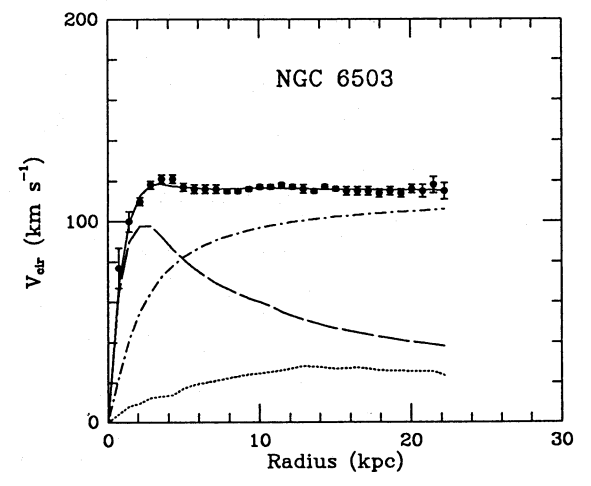
\includegraphics[scale=0.7]{figures/NGC6503_rotcurve.png}
    \caption{Stellar velocity curve fit to NGC 6503 from \cite{Begeman:rot_curves}. Dashed line is the contribution from visible matter. Dotted curves are from gas. Dash-dot curves are from dark matter (DM). Solid line is the composite contribution from all matter and DM sources. Data are indicated with bold dots with error bars. Data agree strongly with a matter + DM composite prediction.}
    \label{fig:gal_rot_curve}
    }
\end{figure}

\Cref{fig:gal_rot_curve} features one of many rotation curves plotted from the stellar velocities within galaxies.
The measured rotation curves mostly feature a flattening of velocities at larder radii which is not expected if the gravity was only coming from luminous matter.
The extension of the flat velocity region also indicates that the DM is distributed far from the center of the galaxy.
Modern velocity measurements include significantly larger objects, galactic clusters, and smaller objects, dwarf galaxies.
Yet, measurements along this regime are leveraging the Virial theorem with Newtonian potential energies.
However, we know Newtonian gravity is not a comprehensive description of gravity.
New observational techniques have been developed since 1978, and those are discussed in the following sections.

%$$$$$$$$$$$$$$$$$$$$$$$$$$$$$$$$$$$$$$$$$$$$$$$$$$$$$$$$$$$$$$$$$$$$$$$$$$$$$$$$$$$%
\subsection{Evidence for Dark Matter: Gravitational Lensing\label{sec:ev4dm_lens}}
%$$$$$$$$$$$$$$$$$$$$$$$$$$$$$$$$$$$$$$$$$$$$$$$$$$$$$$$$$$$$$$$$$$$$$$$$$$$$$$$$$$$%

Modern evidence for dark matter comes from new avenues beyond stellar velocities.
Gravitational lensing from DM is one of these channels from general relativity.
General relativity predicts aberrations in light caused by massive objects.
In recent decades we have been able to measure the lensing effects from compact objects and DM halos.
\Cref{fig:grav_lensing_explained} shows how different massive objects change the final image of a faraway galaxy resulting from gravitational lensing.

\begin{figure}[h!]
    \centering{
        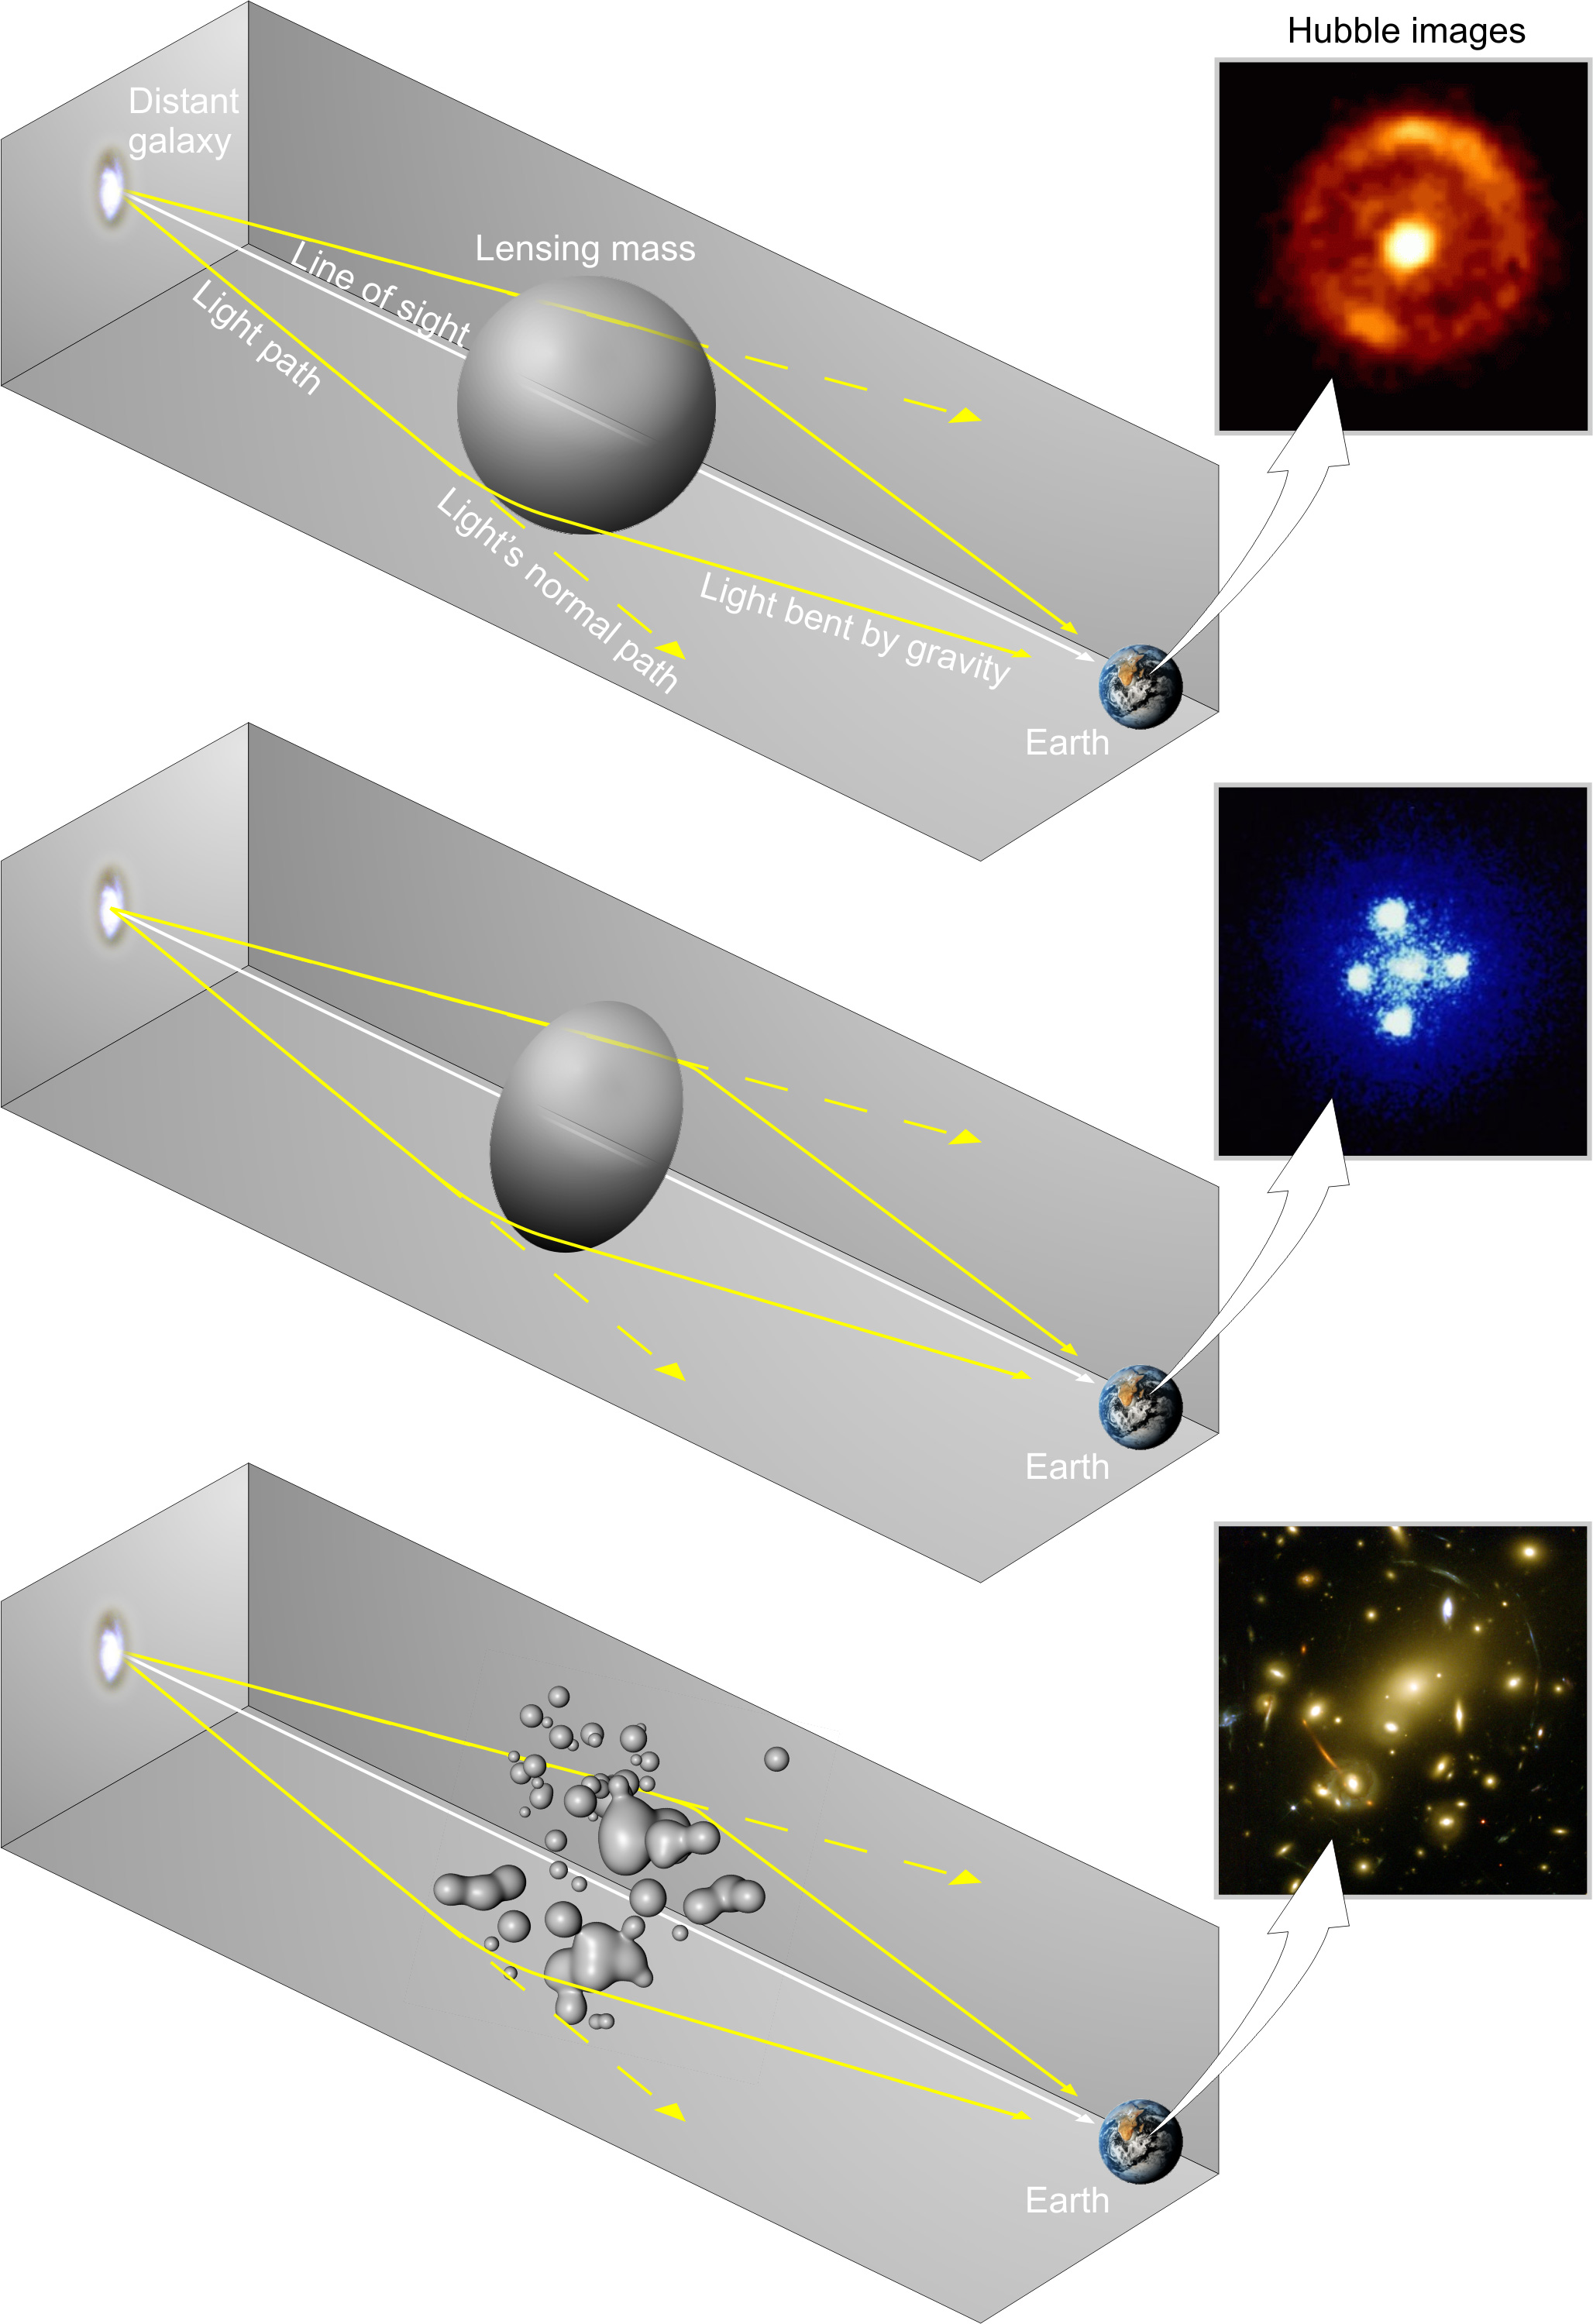
\includegraphics[scale=0.19]{figures/heic0404b.jpg}
        \caption{Light from distant galaxy is bent in unique ways depending on the distribution of mass between the galaxy and Earth. Yellow dashed lines indicate where the light would have gone if the matter were not present. Solid yellow is the path the light actually traverses \cite{eas:grav_lensing}.}
        \label{fig:grav_lensing_explained}
    }
\end{figure}

\begin{figure}[ht]
    \centering{
        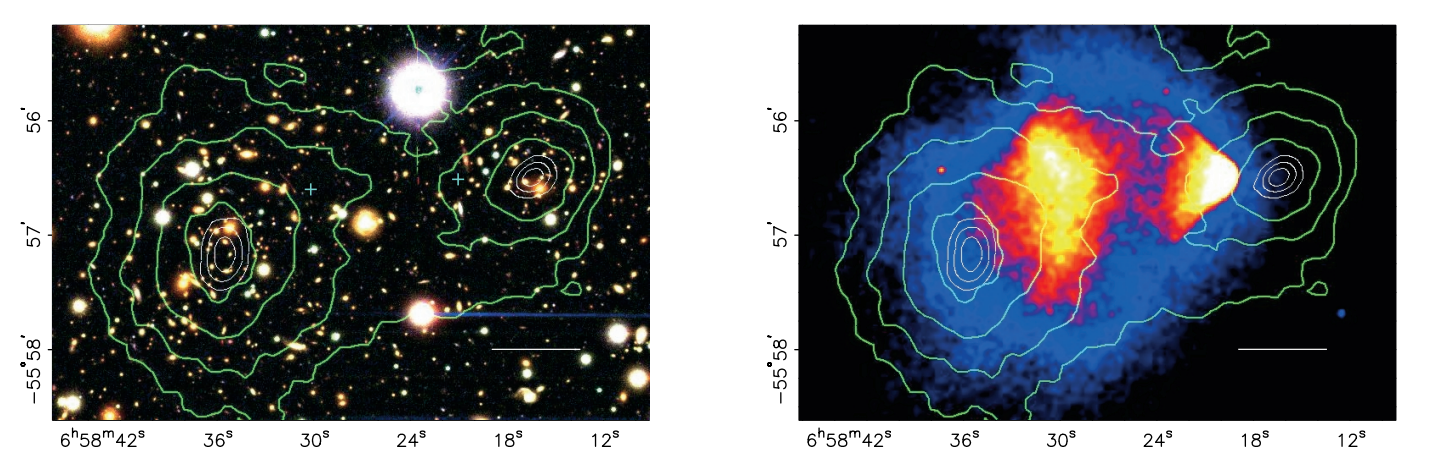
\includegraphics[scale=0.425]{figures/bullet_cluster.png}
        \caption{(left) Optical image of galactic cluster 1E0657-558. (right) X-ray image of the cluster with redder meaning hotter and higher baryon density. (both) Green contours are the reconstructed gravity contours from weak lensing. White rings are the best fit mass maxima at 68.3\%, 95.5\%, and 99.7\% confidence. The matter maxima of the clusters are clearly separated from x-ray maxima. \cite{Clowe:BulletCluster}}
        \label{fig:bullet_cluster}
    }
\end{figure}

Gravitational lensing provides additional compelling evidence for DM.
The observation of two merging galactic clusters in 2006, shown in \Cref{fig:bullet_cluster}, provided a compelling argument for DM outside the Standard Model.
These clusters merged recently in astrophysical time scales.
Galaxies and star cluster have mostly passed by each other as the likelihood of stars colliding within them is low.
Therefore, these massive objects will mostly track the highest mass, dark and/or baryonic, density.
Yet, the intergalactic gas is responsible for the majority of the baryonic mass in the systems \cite{Hooper:DMHistory}.
These gas bodies will not phase through so heat up and compress as they collide together.
The hot gas is located via x-ray emission from the cluster.
Two observations of the clusters were performed independently of each other.

The first was the lensing of light around the galaxies due to their gravitational influences.
When celestial bodies are large enough, the gravity they exert bends space and time itself.
The warped space-time lenses light and will deflect in an analogous way to how glass lenses will bend light, see \Cref{fig:grav_lensing_explained}.
With a sufficient understanding of light sources behind a massive object, we can reconstruct the contours of the gravitational lenses.
The gradient of the contours shown in \Cref{fig:bullet_cluster} then indicates how dense the matter is and where it is.
In the absence of DM, it should also map out where the majority of the mass is.

The x-ray emission is then be observed from the clusters.
Since these galaxies are mostly gas and are merging, the gas should be getting hotter.
If they are merging, the x-ray emissions should be the strongest where the gas is mostly moving through each other.
Hence, X-ray emission maps out where the gas is in the merging galaxy cluster.

The lensing and x-ray observations were done on the Bullet cluster which are featured on \cref{fig:bullet_cluster} \cite{Clowe:BulletCluster}.
The x-ray emissions do not at all align with the gravitational contours.
The incongruence in mass density and baryon density suggests that there is a lot of matter somewhere that does not interact with light.
Moreover, this DM cannot be baryonic \cite{Clowe:BulletCluster}.
The Bullet Cluster measurement did not really tell us what DM is exactly, but it did give the clue that DM also does not interact with itself very strongly.
If DM did interact strongly with itself, then it would have been more aligned with the x-ray emission \cite{Clowe:BulletCluster}.
There have been follow-up studies of galaxy clusters with similar results.
The Bullet Cluster and others like it provide a persuasive case against something possibly amiss in our gravitational theories.

%$$$$$$$$$$$$$$$$$$$$$$$$$$$$$$$$$$$$$$$$$$$$$$$$$$$$$$$$$$$$$$$$$$$$$$$$$$$$$$$$$$$%
\subsection{Evidence for Dark Matter: Cosmic Microwave Background\label{sec:ev4dm_cmb}}
%$$$$$$$$$$$$$$$$$$$$$$$$$$$$$$$$$$$$$$$$$$$$$$$$$$$$$$$$$$$$$$$$$$$$$$$$$$$$$$$$$$$%

\begin{figure}[h]
    \centering{
        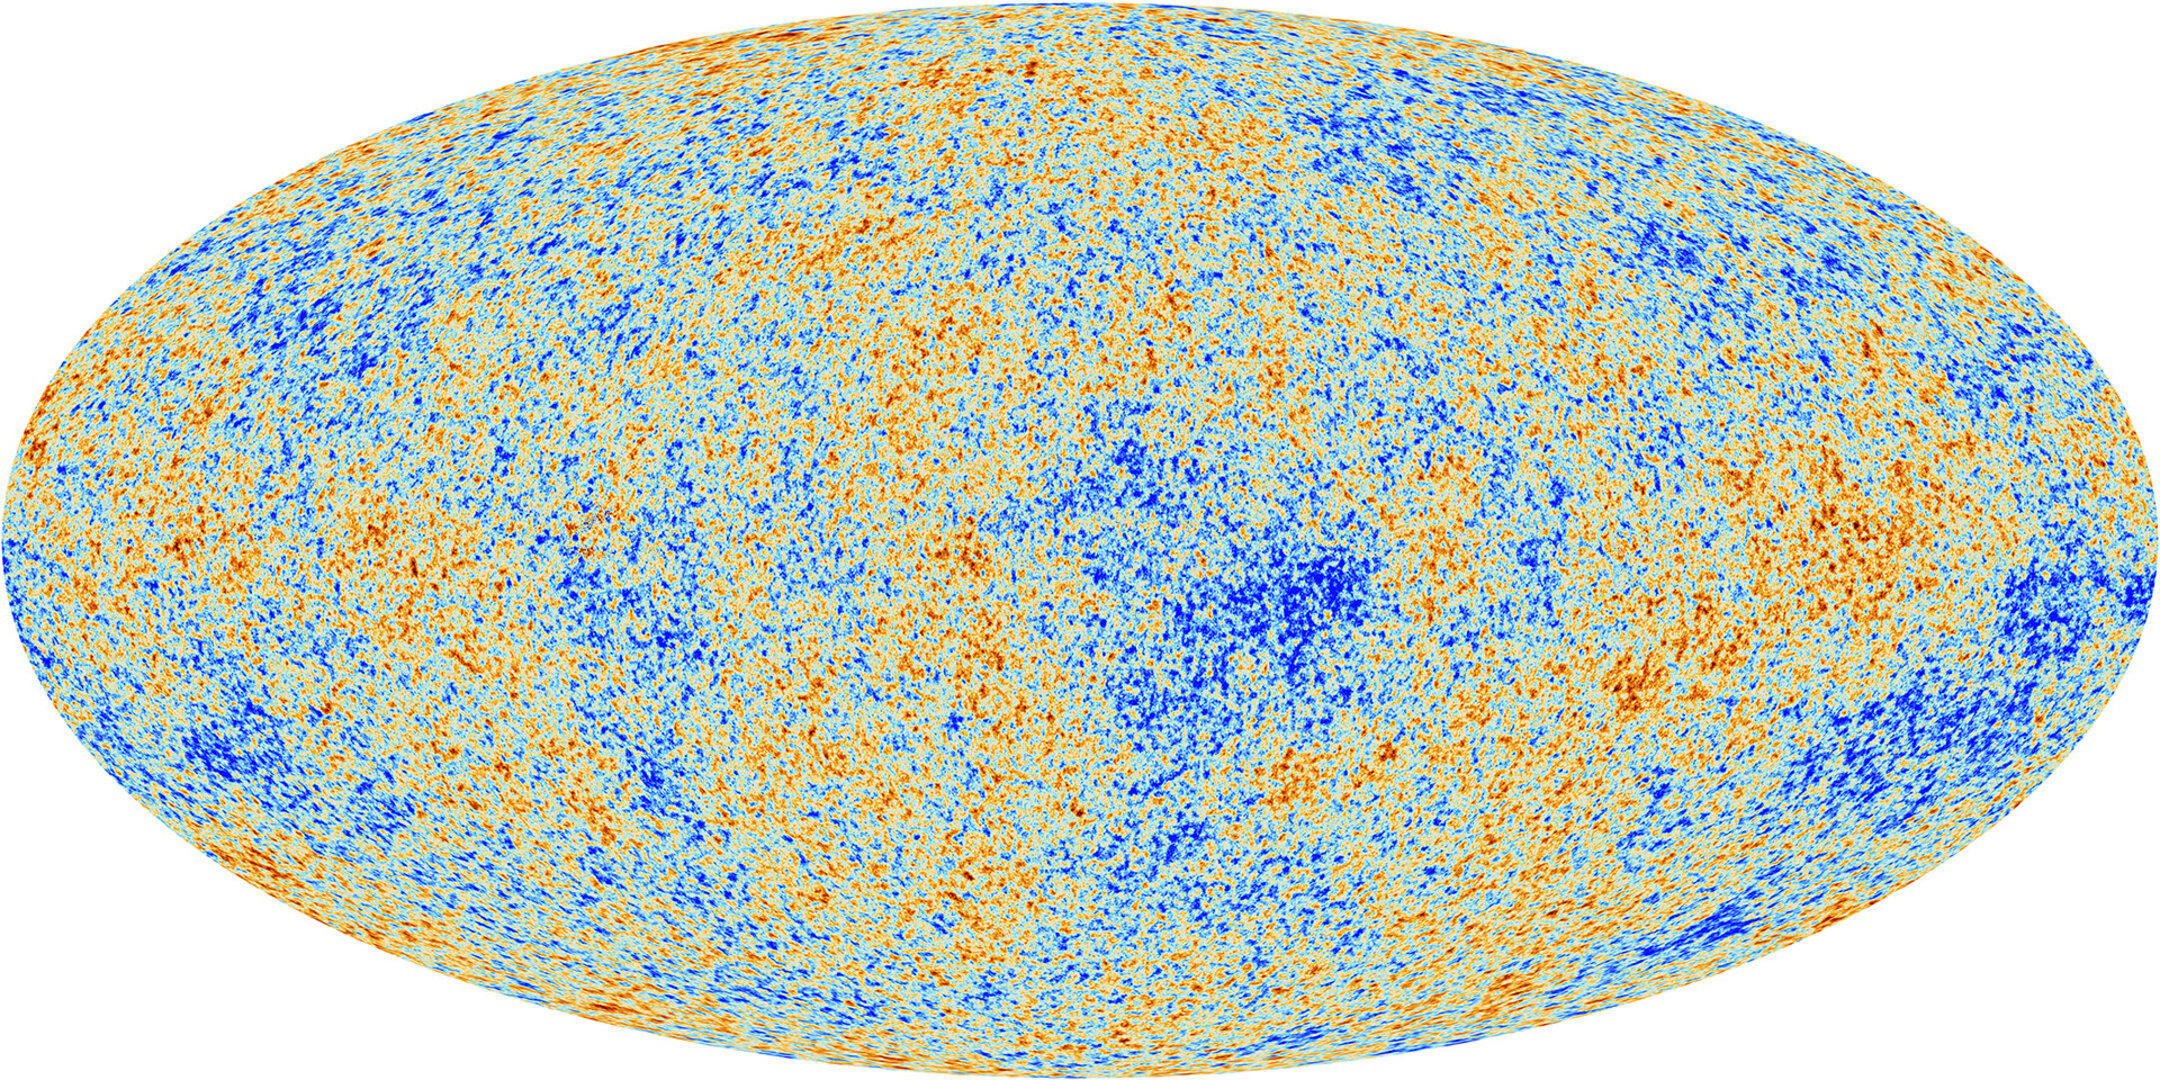
\includegraphics[scale=0.215]{figures/Planck_CMB_pillars.jpg}
        \caption{Plank CMB sky. Sky map features small variations in temperature in primordial light. These anisotropies are used to make inferences about the universe's energy budget and developmental history. \cite{Plank:CMB}}
        \label{fig:CMB}
    }
\end{figure}

The Cosmic Microwave Background (CMB) is the primordial light from the early universe when Hydrogen atoms formed from the combination of free electron and proton soup in the early universe.
Prior to this recombination, the universe was too hot to form atoms and was opaque to light.
The CMB is the earliest light we can observe; released when the universe was about 380,000 years old.
Then we look at how the simulated universes look like compared to what we see.
\Cref{fig:CMB} is the most recent CMB image from the Plank satellite after subtracting the average value and masking the galactic plane \cite{Plank:CMB}.
Redder regions indicate a slightly hotter region in the CMB, and blue indicates colder.
The intensity variations are on the order of 1 in 1000 with respect to the average value.

\begin{figure}[ht]
    \centering{
        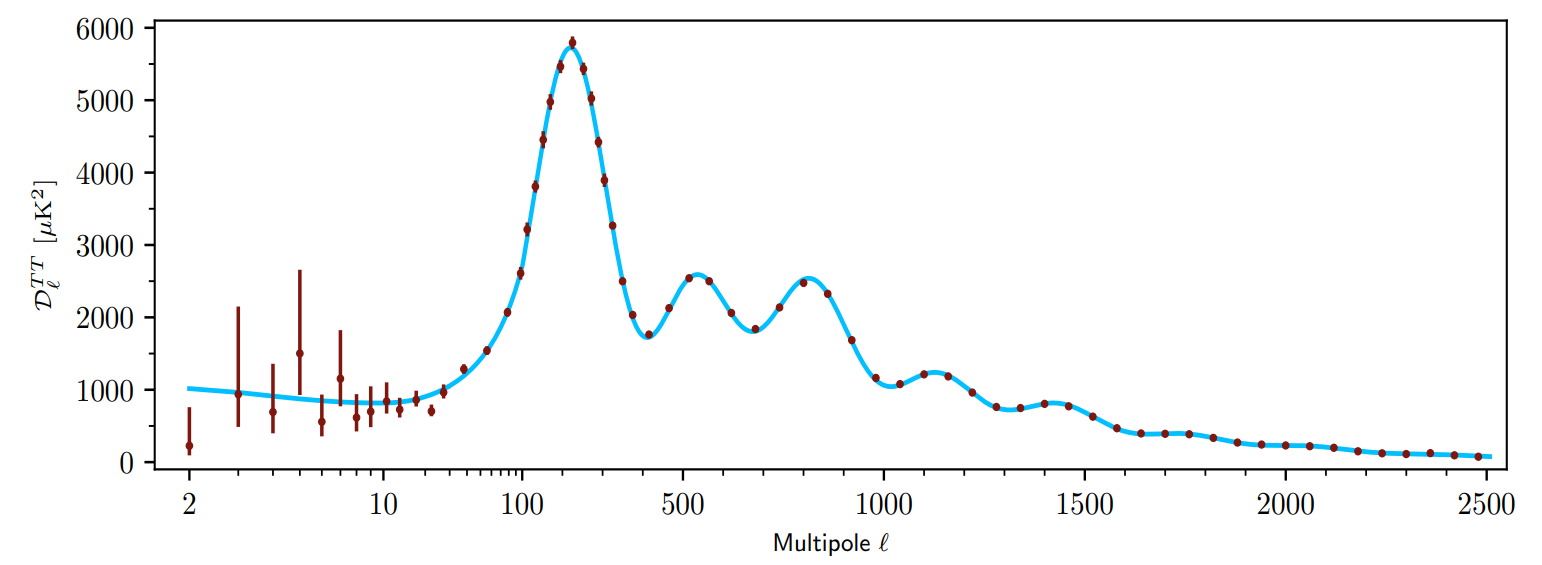
\includegraphics[scale=0.4]{figures/multipole.png}
        \caption{Observed Cosmic Microwave Background power spectrum as a function of multipole moment from Plank observatory \cite{Plank:CMB}. Blue line is the best fit model from \lcdm. Red points and lines are data and error, respectively. }
        \label{fig:multipole}
    }
\end{figure}

The Cosmic Microwave Background shows that the universe had DM in it from an incredibly early stage.
To measure the DM, Dark Energy, and matter fractions of the universe from the CMB, the image is analyzed into a power spectrum, which shows the amplitude of the fluctuations as a function of spherical multipole moments.
\lcdm~provides the best fit to the power spectra of the CMB as shown in \cref{fig:multipole}.
The CMB power spectrum is quite sensitive to the fraction of each energy contribution in the early universe.
Low \textit{l} modes are dominated by variations in gravitational potential.
Intermediate \textit{l} emerge from oscillations in the photon-baryon fluid from competing baryon pressures and gravity.
High \textit{l} is a damped region from the diffusion of photons during electron-proton recombination. \cite{Greene:cosmology_dm}

\begin{figure}[ht]
    \centering{
        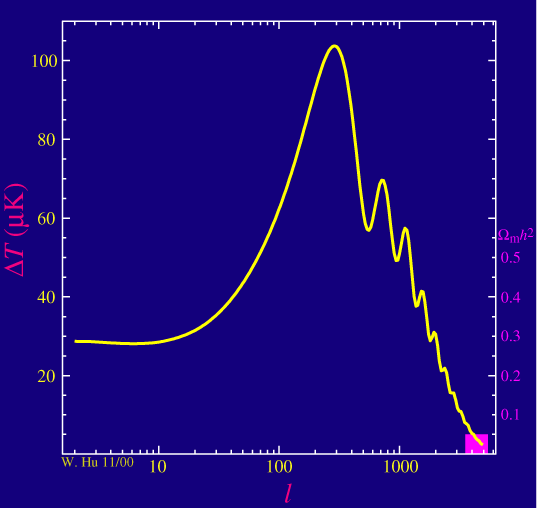
\includegraphics[scale=0.285]{figures/LCDM_multipole/frame_00_delay-0.2s.png}\hfill
        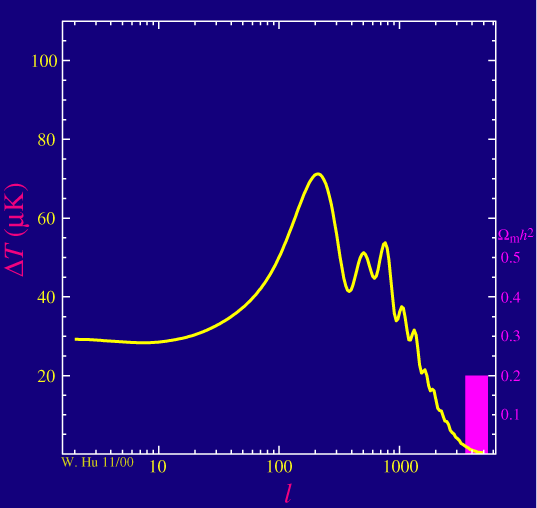
\includegraphics[scale=0.285]{figures/LCDM_multipole/frame_06_delay-0.2s.png}\hfill
        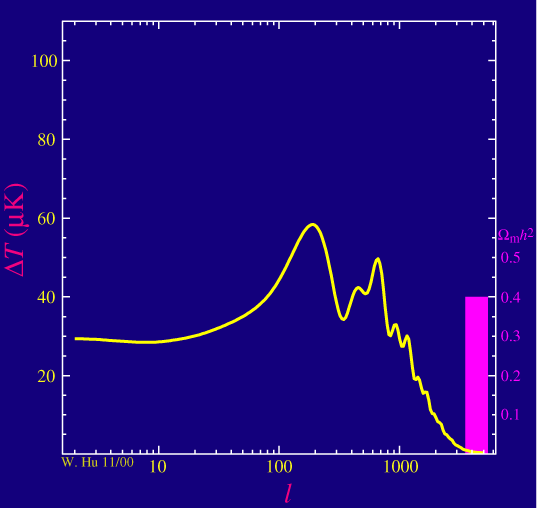
\includegraphics[scale=0.285]{figures/LCDM_multipole/frame_16_delay-0.2s.png}
        \caption{Predicted power spectra of CMB for different $\Omega_m h^2$ values for fixed baryon density from \cite{waynehu:dm_anim}. (left) Low $\Omega_m h^2$ increases the prominence of first and second peaks. (middle) $\Omega_m h^2$ is most similar to the observed power spectrum. The second and third peaks are similar in height. (right) $\Omega_mh^2$ is large which suppresses the first peak and raises the prominence of the third peak.}
        \label{fig:CMB_vibratemodes}
    }
\end{figure}

The harmonics would look quite different for a universe with less DM.
\Cref{fig:CMB_vibratemodes} demonstrates the effect $\Omega_m h^2$, the mass fraction, has on the expected power spectrum for fixed baryon matter density. \cite{waynehu:dm_anim}
Sweeping  $\Omega_m h^2$ while keeping the baryon mass fraction fixed clearly shows the effect dark matter has on the CMB power spectrum.
The observations fit well with the \lcdm~model, and the derived fractions are as follows.
The matter fraction: $\Omega_m = 0.3153$; and the baryon fraction: $\Omega_b = 0.04936$ \cite{Plank:CMB}.
Plank's observations also provide a measure of the Hubble constant, $H_0$.
$H_0$ especially has seen a growing tension in the past decade that continues to deepened with observations from instruments like the James Webb Telescope \cite{JWST:hubble_tension,Freedman:hubble_tension}.
As Hubble tensions deepen, we may find that perhaps \lcdm, despite its successes, is missing some critical physics.

Overall, the Newtonian motion of stars in galaxies, weak lensing from galactic clusters, and power spectra from primordial light form a compelling body of research in favor of dark matter.
It takes another leap of theory and experimentation to make observations of DM that are non-gravitational in nature.
In \cref{sec:evidence4dm}, the evidence for DM implies strongly that the DM is matter and not a lost parameter in the gravitational fields between massive objects.
Finally, if we take one axiom: that this matter has quantum behavior, such as being described by some Bohr wavelength and abiding by some fermion or boson statistics; then we arrive at particle dark matter.
One particle DM hypothesis is the Weakly Interacting Massive Particle (WIMP).
This DM candidate theory is discussed further in the next section and is the focus of this thesis.

%-----------------------------------------------------------------------------------%
\section{Searching for Dark Matter: Particle DM}\label{sec:dm_search}
%-----------------------------------------------------------------------------------%

\begin{figure}[h]
    \centering{
        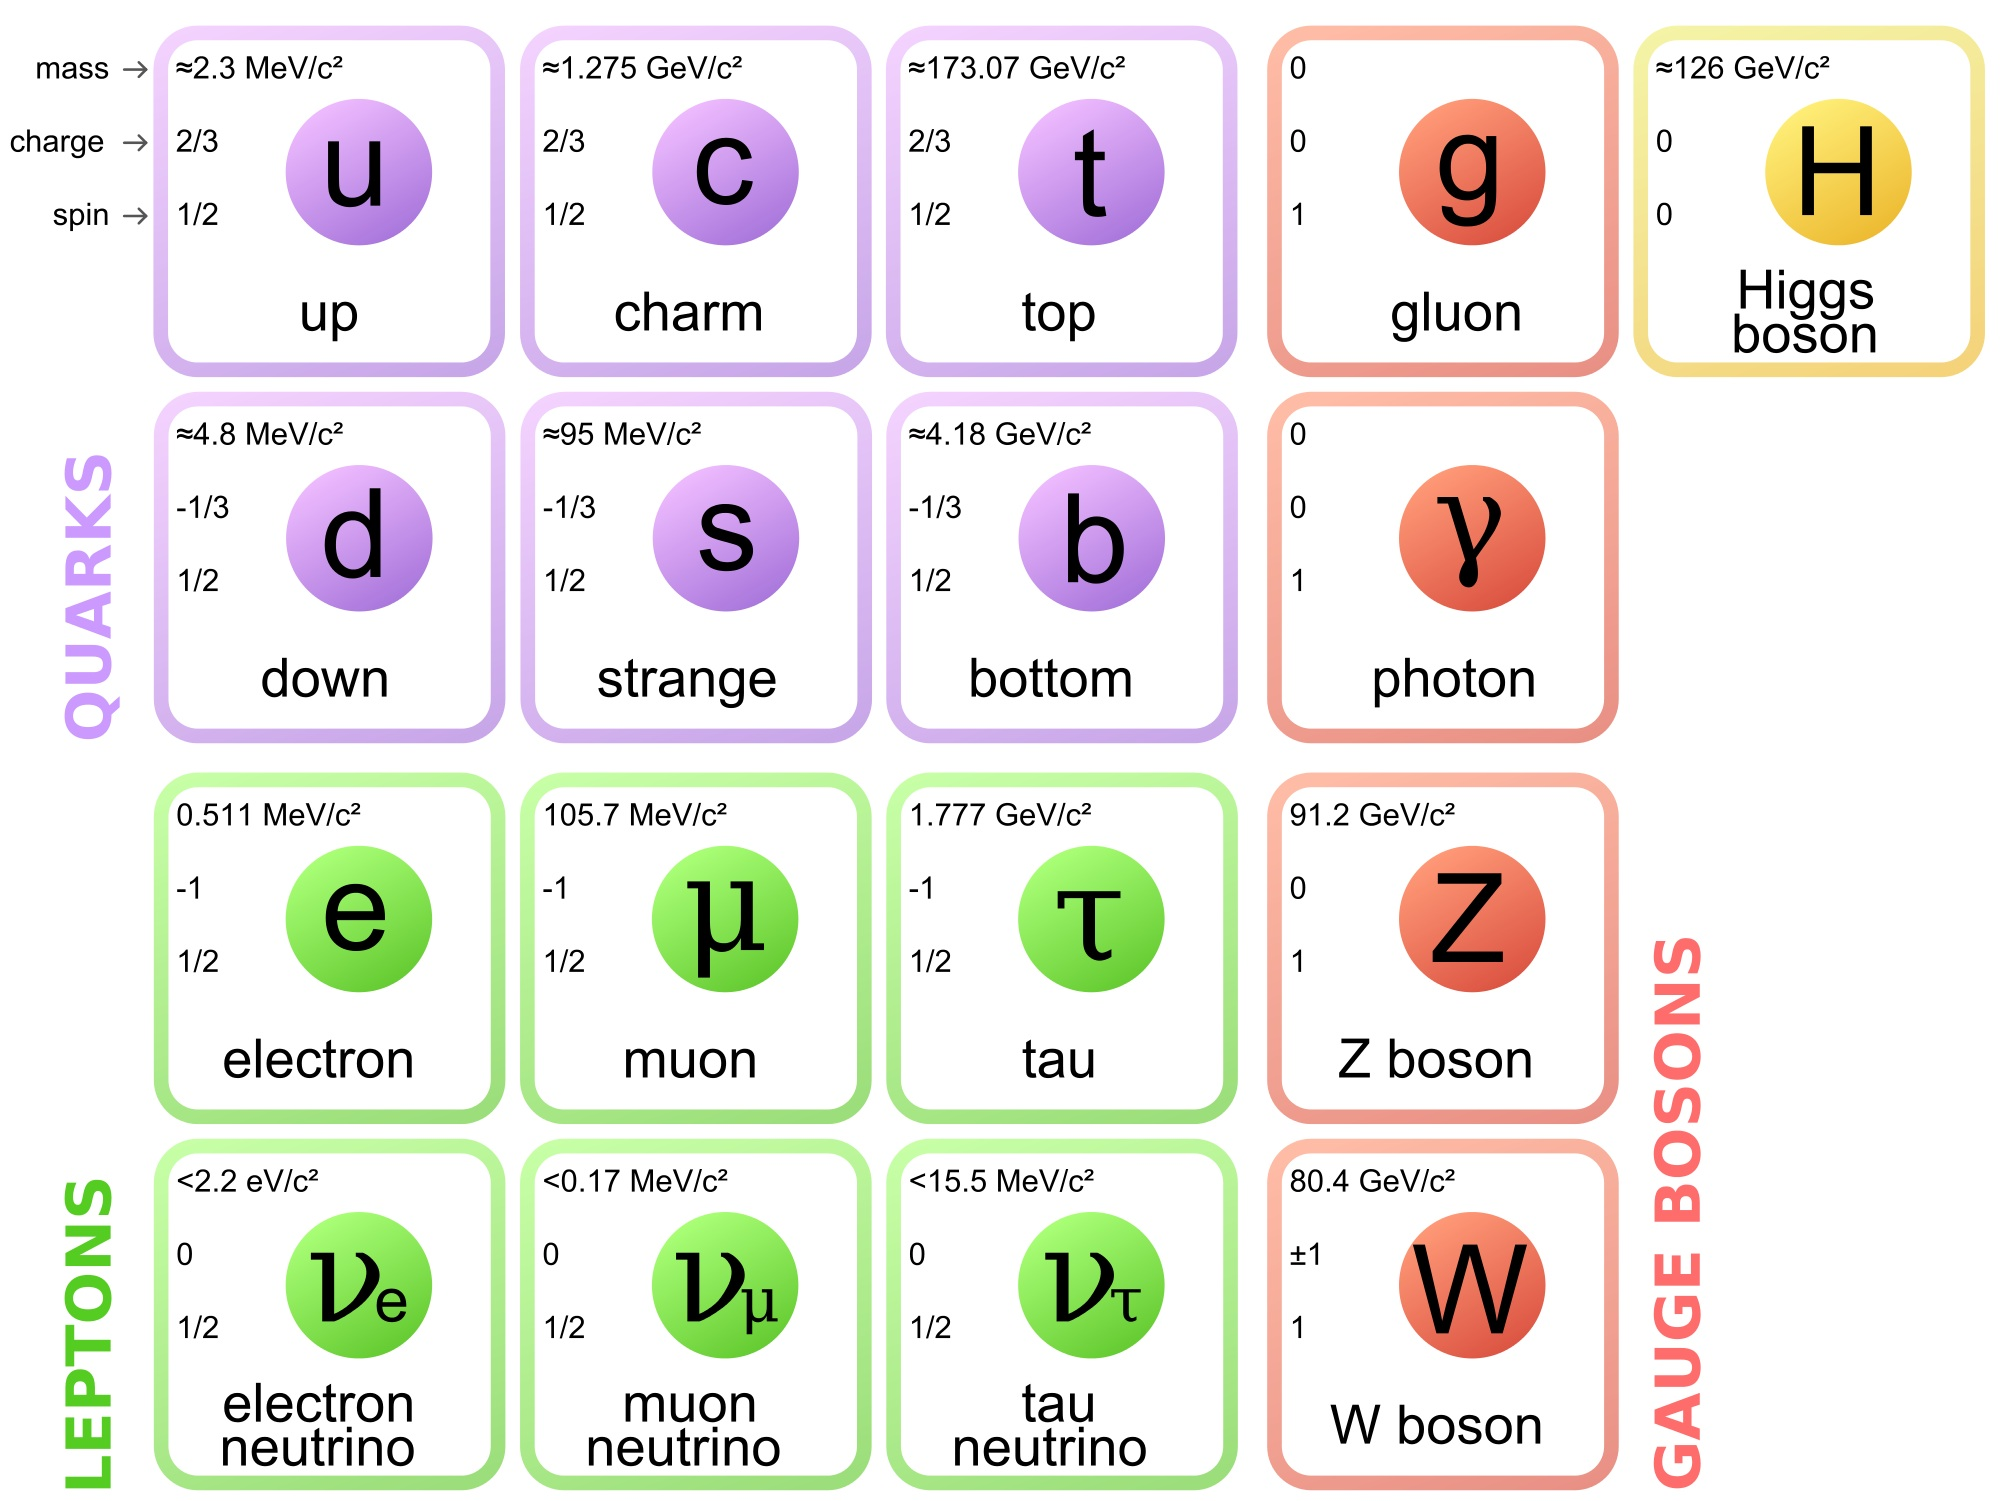
\includegraphics[scale=0.225]{figures/SM.jpg}
    }
    \caption{The Standard Model (SM) of particle physics. Figure taken from \cite{sm_table}}
    \label{fig:SM}
\end{figure}

\Cref{fig:SM} shows the Standard Model of particle physics and is currently the most accurate model for the dynamics of fundamental particles like electrons and photons.
The current status of the SM does not have a viable DM candidate.
When looking at the standard model, we can immediately exclude any charged particle because charged particles interact strongly with light.
Specifically, this will rule out the following charged, fundamental particles: $e,\mu, \tau, W, u, d, s, c, t, b$ and their corresponding antiparticles.
Recalling from \cref{sec:basicDM} that DM must be long-lived and stable over the age of the universe, we exclude all SM particles with decay half-lives at or shorter than the age of the universe.
The lifetime constraint additionally eliminates the $Z$ and $H$ bosons.
Finally, the candidate DM needs to be somewhat massive.
Recall from \Cref{sec:basicDM} that DM is cold or not relativistic through the universe.
This eliminates the remaining SM particles: $\nu_{e, \mu, \tau}, g, \gamma$ as DM candidates.
Because there are no DM candidates within the SM, the DM problem strongly hints to physics beyond the SM (BSM).

%$$$$$$$$$$$$$$$$$$$$$$$$$$$$$$$$$$$$$$$$$$$$$$$$$$$$$$$$$$$$$$$$$$$$$$$$$$$$$$$$$$$%
\subsection{Shake it, Break it, Make it\label{sec:bop_it}}
%$$$$$$$$$$$$$$$$$$$$$$$$$$$$$$$$$$$$$$$$$$$$$$$$$$$$$$$$$$$$$$$$$$$$$$$$$$$$$$$$$$$%

\begin{figure}[h]
    \centering{
        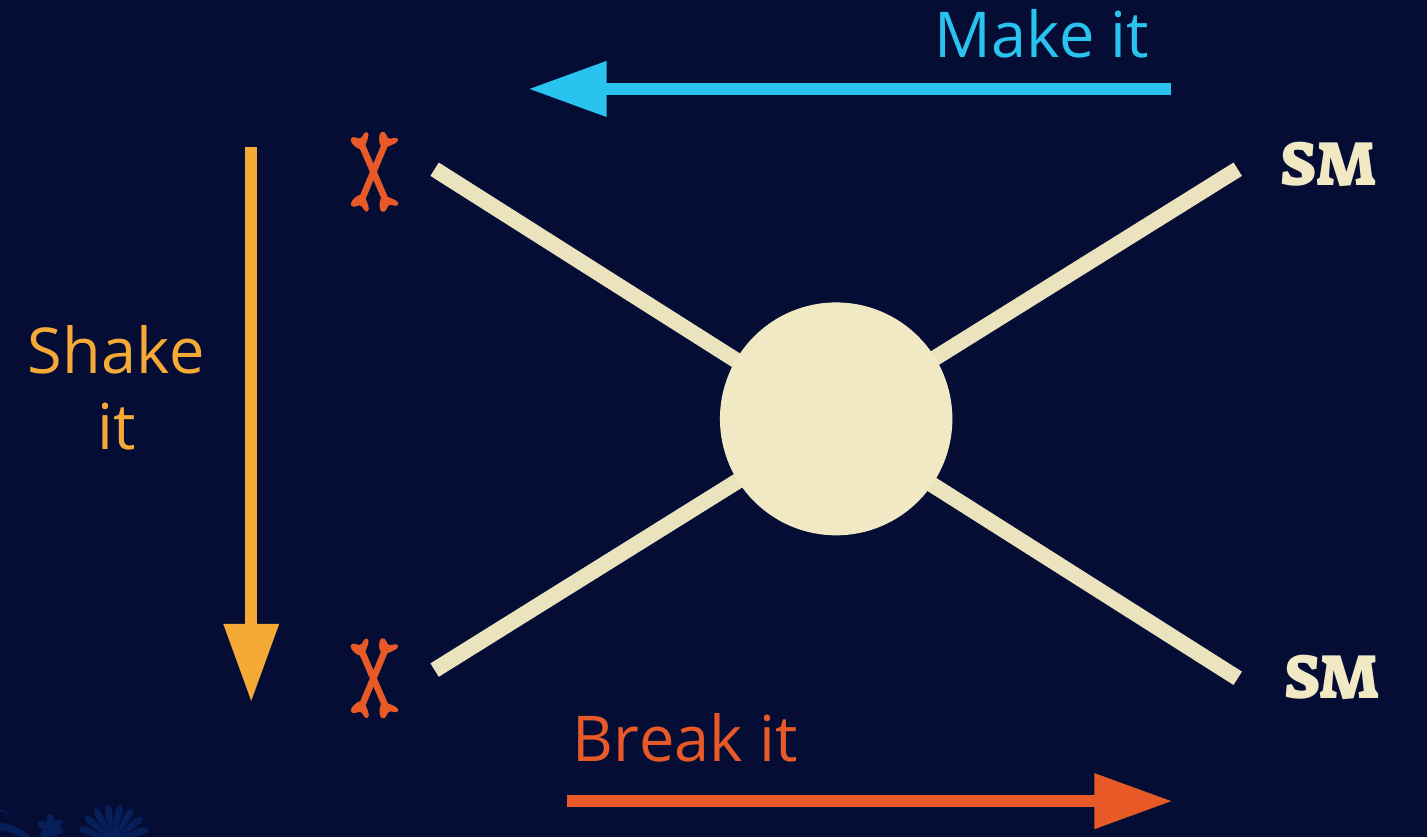
\includegraphics[scale=0.38]{figures/DM_with_SM.png}
        \caption{Simplified Feynman diagram demonstrating the different ways DM can interact with SM particles. The 'X's refer to the DM particles whereas the SM refer to fundamental particles in the SM. The large circle in the center indicates the vertex of interaction and is purposely left vague. The colored arrows refer to different directions of time as well as their respective labels.}
        \label{fig:break_it}
    }
\end{figure}

When considering DM that couples in some way with the SM, the interactions are roughly demonstrated by interaction demonstrated in \Cref{fig:break_it}.
The figure is a simplified Feynman diagram where the arrow of time represents the interaction modes of: \textbf{Shake it, Break it, Make it}.

\textbf{Shake it} refers to the direct detection of dark matter.
Direct detection interactions start with a free DM particle and an SM particle.
The DM and SM interact via elastic or inelastic collision and recoil away from each other.
The DM remains in the dark sector and imparts some momentum onto the SM particle.
The hope is that the momentum imparted onto the SM particle is sufficiently high enough to pick up with extremely sensitive instruments.
Because we cannot create the DM in the lab, a direct detection experiment must wait until DM is incident on the detector.
Most direct detection experiments are therefore placed in low-background environments with inert detection media like the noble gas, Xenon. \cite{Cooley:dd_dm}

\textbf{Make it} refers to the production of DM from SM initial states.
The experiment starts with particles in the SM.
These SM particles are accelerated to incredibly high energies and then collide with each other.
In the confluence of energy, DM hopefully emerges as a byproduct of the SM annihilation.
Often it is the collider experiments that are energetic enough to hypothetically produce DM.
These experiments include the world-wide collaborations, ATLAS and CMS at CERN, where protons collide together at extreme energies.
The DM searches, however, are complex.
DM likely does not interact with the detectors and lives long enough to escape the detection apparatus of CERN's colliders.
This means any DM production experiment searches for an excess of events with missing momentum or energy in the events.
An example event with missing transverse momentum is shown in \Cref{fig:met_atlas}.
The missing momentum with no particle tracks implies a weakly interacting particle carried the energy out of the detector.
However, there are other neutral particles in the SM, like neutrons or neutrinos, so any analysis has to account for SM signatures of missing momentum. \cite{atlas:met_dm_precise}

\begin{figure}[h]
    \centering{
        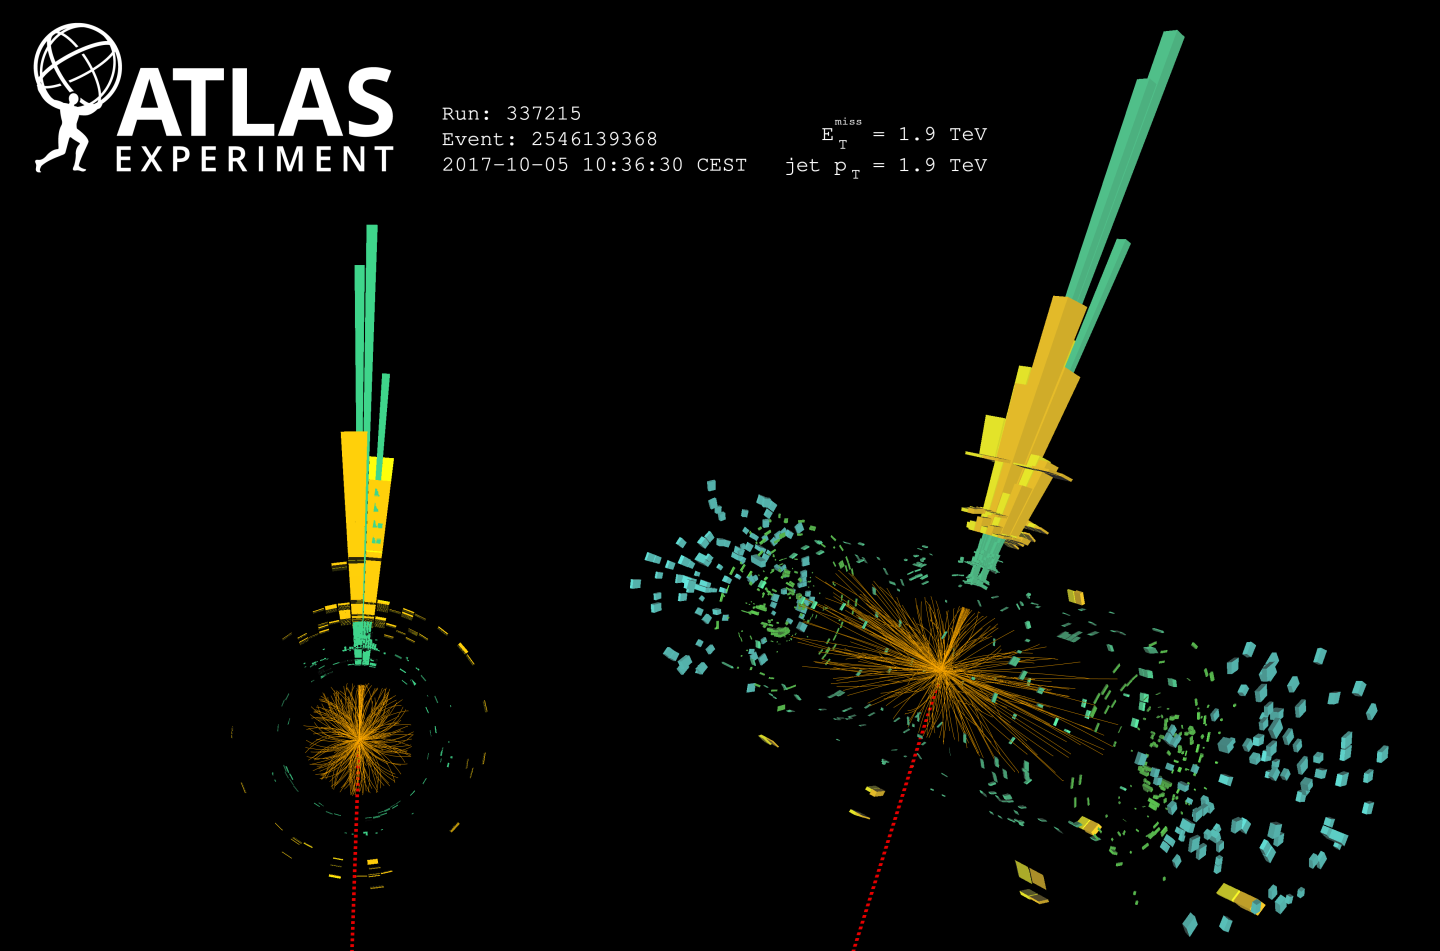
\includegraphics[scale=0.435]{figures/MET_ATLAS.png}
        \caption{A single jet event in the ATLAS detector from 2017 \cite{atlas:dm_precise}. Total transverse momentum was observed to be 1.9 TeV where it should be 0. Missing transverse momentum is inferred to be opposite the observed transverse momentum in order to preserve overall momentum in the event.}
        \label{fig:met_atlas}
    }
\end{figure}

%$$$$$$$$$$$$$$$$$$$$$$$$$$$$$$$$$$$$$$$$$$$$$$$$$$$$$$$$$$$$$$$$$$$$$$$$$$$$$$$$$$$%
\subsection{Break it: Standard Model Signatures of Dark Matter through Indirect Searches\label{sec:break_it}}
%$$$$$$$$$$$$$$$$$$$$$$$$$$$$$$$$$$$$$$$$$$$$$$$$$$$$$$$$$$$$$$$$$$$$$$$$$$$$$$$$$$$%

\textbf{Break it} refers to the creation of SM particles from the dark sector, and it is the primary focus of this thesis.
The interaction begins with DM in the dark sector.
The hypothesis is that this DM will either annihilate with itself or decay and produce an SM byproduct.
This method is often referred to as the Indirect Detection of DM because we have no lab to directly control or manipulate the DM.
Therefore, most indirect DM searches are performed using observations of known DM densities among astrophysical sources.
The strength is that we have the whole of the universe and its 13.6-billion-year lifespan to use as a detector and particle accelerator.
Additionally, locations of dark matter are well cataloged since it was astrophysical observations that presented the problem of DM in the first place.

\begin{figure}[ht]
    \centering{
        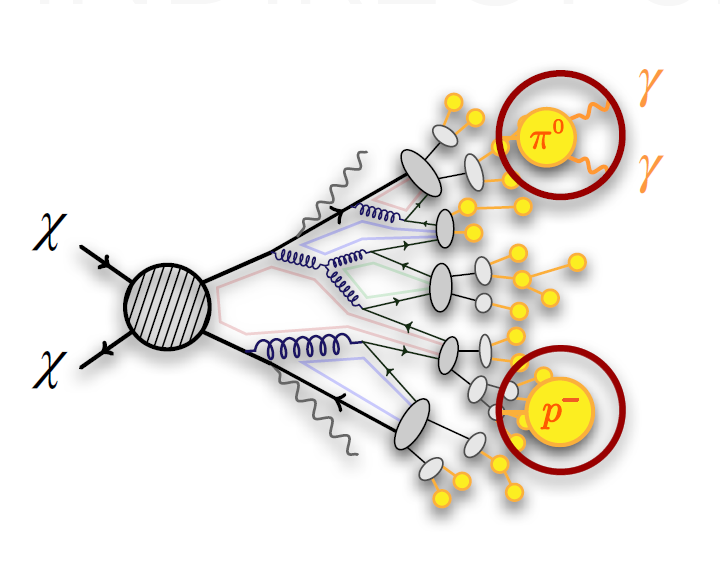
\includegraphics[scale=0.4]{figures/DM_annihilation.png}
        \caption{More detailed pseudo-Feynman diagram of particle cascade from dark matter annihilation into 2 quarks. The quarks hadronize down to stable particles like \textgamma~or the anti-proton ($p^-$). Diagram pulled from ICRC 2021 presentation on DM annihilation search \cite{2021ICRC:glory_duck}.}
        \label{fig:id_dm_ann}
    }
\end{figure}

However, anything can happen in the universe.
There are many difficult to deconvolve backgrounds when searching for DM.
One prominent example is the galactic center.
We know the galactic center has a large DM content because of stellar kinematics in our Milky Way and DM halo simulations.
Yet, any signal from the galactic center is challenging to parse apart from the extreme environment of our supermassive black hole, unresolved sources, and diffuse emission from the interstellar medium \cite{Tracy:les_houches}.
Despite the challenges, any DM model that yields evidence in the other two observation methods, \textbf{Shake it} or \textbf{Make it} must be corroborated with indirect observations of the known DM sources.
Without corroborating evidence, DM observation in the lab is hard-pressed to demonstrate that it is the model contributing to the DM seen at the universal scale.

In the case of WIMP DM, signals are described in terms of primary SM particles produced from DM decay or annihilation.
The SM initial state particles are then simulated down to stable final states such as the $\gamma, \nu, p, \text{or } e$ which can traverse galactic lengths to reach the Earth.

\Cref{fig:id_dm_ann} shows the quagmire of SM particles that emerges from SM initial states that are not stable \cite{2021ICRC:glory_duck}.
There are many SM particles with varying energies that can be produced in such an interaction.
For any arbitrary DM source and stable SM particle, the SM flux from DM annihilating to a neutral particle in the SM, $\phi$, from a region in the sky is described by the following.
\iddmannilationPhi
In \cref{eq:id_dm_flux_phi}, \sv~is the velocity-weighted annihilation cross-section of DM to the SM.
$m_\chi$ refers to the mass of DM, noted with Greek letter $\chi$.
$\frac{dN_{\phi}}{dE_\phi}$ is the N particle flux weighted by the particle energy.
Example spectra are provided in \cref{fig:dm_decay_spectra} for the $\chi\chi \rightarrow$ \parpar{b} $\rightarrow \gamma$ final state.
The integrated terms are performed over the solid angle, $d\Omega$, and line of sight, l.o.s.
$\rho$ is the density of DM for a location $(r, \theta')$ in the sky.
The terms left of the '$\times$' are often referred to as the particle physics component.
The terms on the right are referred to as the astrophysical component.
For decaying DM, the equation changes to\dots
\iddmdecay

In \Cref{eq:id_dm_decay}, $\tau$ is the decay lifetime of the DM.
Just as in \cref{eq:id_dm_flux_phi}, the left and right terms are the particle physics and the astrophysical components respectively.
The integrated astrophysical component of \cref{eq:id_dm_flux} is often called the J-Factor.
Whereas the integrated astrophysical component of \cref{eq:id_dm_decay} is often called the D-Factor.

\begin{figure}[h]
    \centering{
        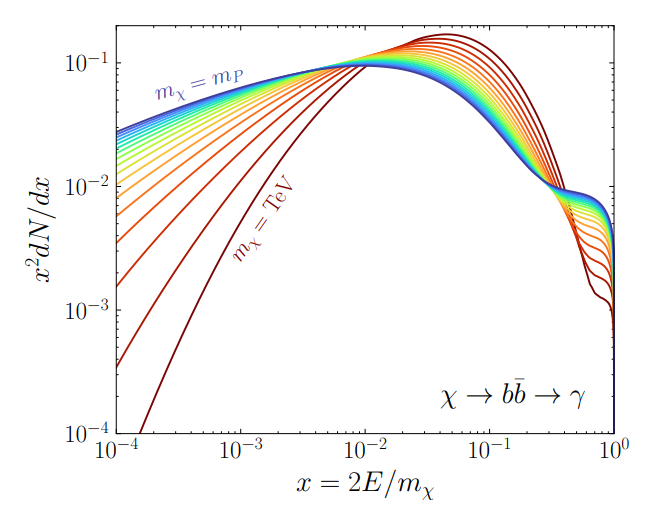
\includegraphics[scale=0.65]{figures/bb_decay_hdm.png}
        \caption{Dark Matter (DM) decay spectrum for $b\bar{b}$ initial state and $\gamma$ final state. Redder spectra are for larger DM masses. Bluer spectra are light DM masses. $x$ is a unitless factor defined as the ratio of the mass of DM, $m_\chi$, and the final state particle energy $E_{\gamma}$. Figure from \cite{Rodd:HDM_spec}.}
        \label{fig:dm_decay_spectra}
    }
\end{figure}

Exact $\chi\chi \rightarrow$ \textbf{SM SM} branching ratios are not known, so it is usually assumed to go 100\% into an SM particle/anti-particle.
Additionally, when a DM annihilation or decay produces one of the neutral, long-lived SM particles ($\nu$ or $\gamma$), the particle can be traced back to a DM source.
For DM above GeV energies, there are very few SM processes that can produce particles with such a high energy.
Seeing such a signal would almost certainly be an indication of the presence of dark matter.
Fortunately, the universe  provides us with the largest volume and lifetime ever for a particle physics experiment.

%-----------------------------------------------------------------------------------%
\section{Sources for Indirect Dark Matter Searches\label{sec:dm_targets}}
%-----------------------------------------------------------------------------------%

\begin{figure}
    \centering{
        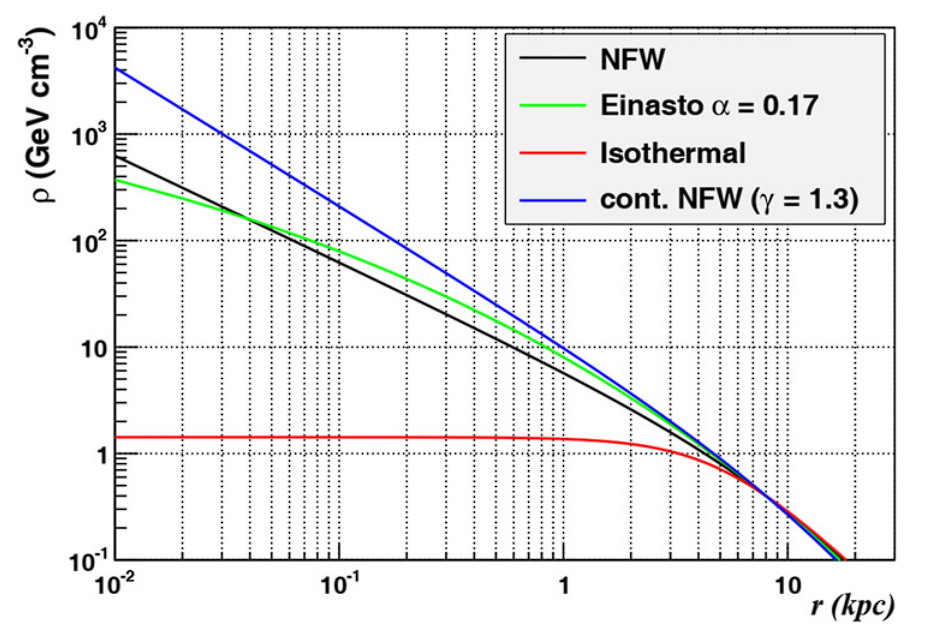
\includegraphics[scale=0.5]{figures/dm_profiles.png}
        \caption{Different dark matter density profiles compared. Some models produce exceptionally large densities at small r \cite{2010:dm_profiles}.}
        \label{fig:dm_profile}
    }
\end{figure}

The first detection of DM relied on optical observations.
Since then, we have developed new techniques to find DM dense regions.
As described in \cref{sec:ev4dm_stars}, many DM dense regions were discovered through observing galactic rotation curves.
Our Milky Way galaxy is among DM dense regions discovered, and it is the largest nearby DM dense region to look at.
Additionally, the DM halo surrounding the Milky Way is clumpy \cite{Tracy:les_houches}.
There are regions in the DM halo of the Milky Way that have more DM than others that have captured gas over time.
These sub-halos were dense enough collapse gas and form stars.
These apparent sub galaxies are known as dwarf spheroidal galaxies (dSphs) and are the main sources studied in this thesis.
Each source type comes with different trade-offs.
Galactic Center studies will be very sensitive to the assumed distribution of DM.
The central DM density can vary substantially as demonstrated in \cref{fig:dm_profile}.
At distances close to the center of the galaxy, or small \textit{r}, the differences in DM densities can be 3-4 orders of magnitude.
Searches toward the galactic center will therefore be quite sensitive to the assumed DM distribution.

Searches dSphs suffer from uncertainties in the DM density less than the galactic center studies.
This is mostly from their diminutive size being smaller than the angular resolution of most high energy astrophysical observatories \cite{Tracy:les_houches}.
The DM content of dSphs are typically determined with the Virial theorem, \cref{eq:virialtheorem}, and are usually majority DM \cite{Tracy:les_houches} in mass.
DSph's tend to be ideal sources to look at for DM searches.
Their environments are quiet with little astrophysical background.
Unlike the galactic center, the most energetic components of dSph's are the stars within them versus a violent accretion disc around a black hole.
All this together means that dSph's are among the best sources to look at for indirect DM searches.
dSph's are the targets of focus for this thesis.

%-----------------------------------------------------------------------------------%
\section{Multi-Messenger Dark Matter \label{sec:mult-messengerDM}}
%-----------------------------------------------------------------------------------%

Astrophysics entered a new phase in the past few decades that leverages our increasing sensitivity to SM channels and general relativity (GR).
Up until the 21st century, astrophysical observations were performed with photons ($\gamma$) only.
Astrophysics with this 'messenger' is fairly mature now.
Novel observations of the universe have since only adjusted the sensitivity of the wavelength of light that is observed except at MeV energies.
Gems like the CMB \cite{Plank:CMB}, and more have ultimately been observations of different wavelengths of light.
Multi-messenger astrophysics proposes using other SM particles such the $p^{+/-},  \nu$, or gravitation waves predicted by general relativity.

The experiment LIGO had a revolutionary discovery in 2016 with the first detection of a binary black hole merger \cite{2016:grav_waves}.
This opened the collective imagination to observing the universe through gravitational waves.
There has also been a surge of interest in the neutrino ($\nu$) sector.
IceCube demonstrated that we are sensitive to neutrinos in regions that correlate with significant photon emission like the galactic plane \cite{2023:IC3_galactic_plane}.
Neutrinos, like gravitational waves and light, travel mostly unimpeded from their source to our observatories.
This makes pointing to the originating source of these messengers much easier than it is for cosmic rays which are deflected from their source by magnetic fields.

\begin{figure}[h]
    \centering{
        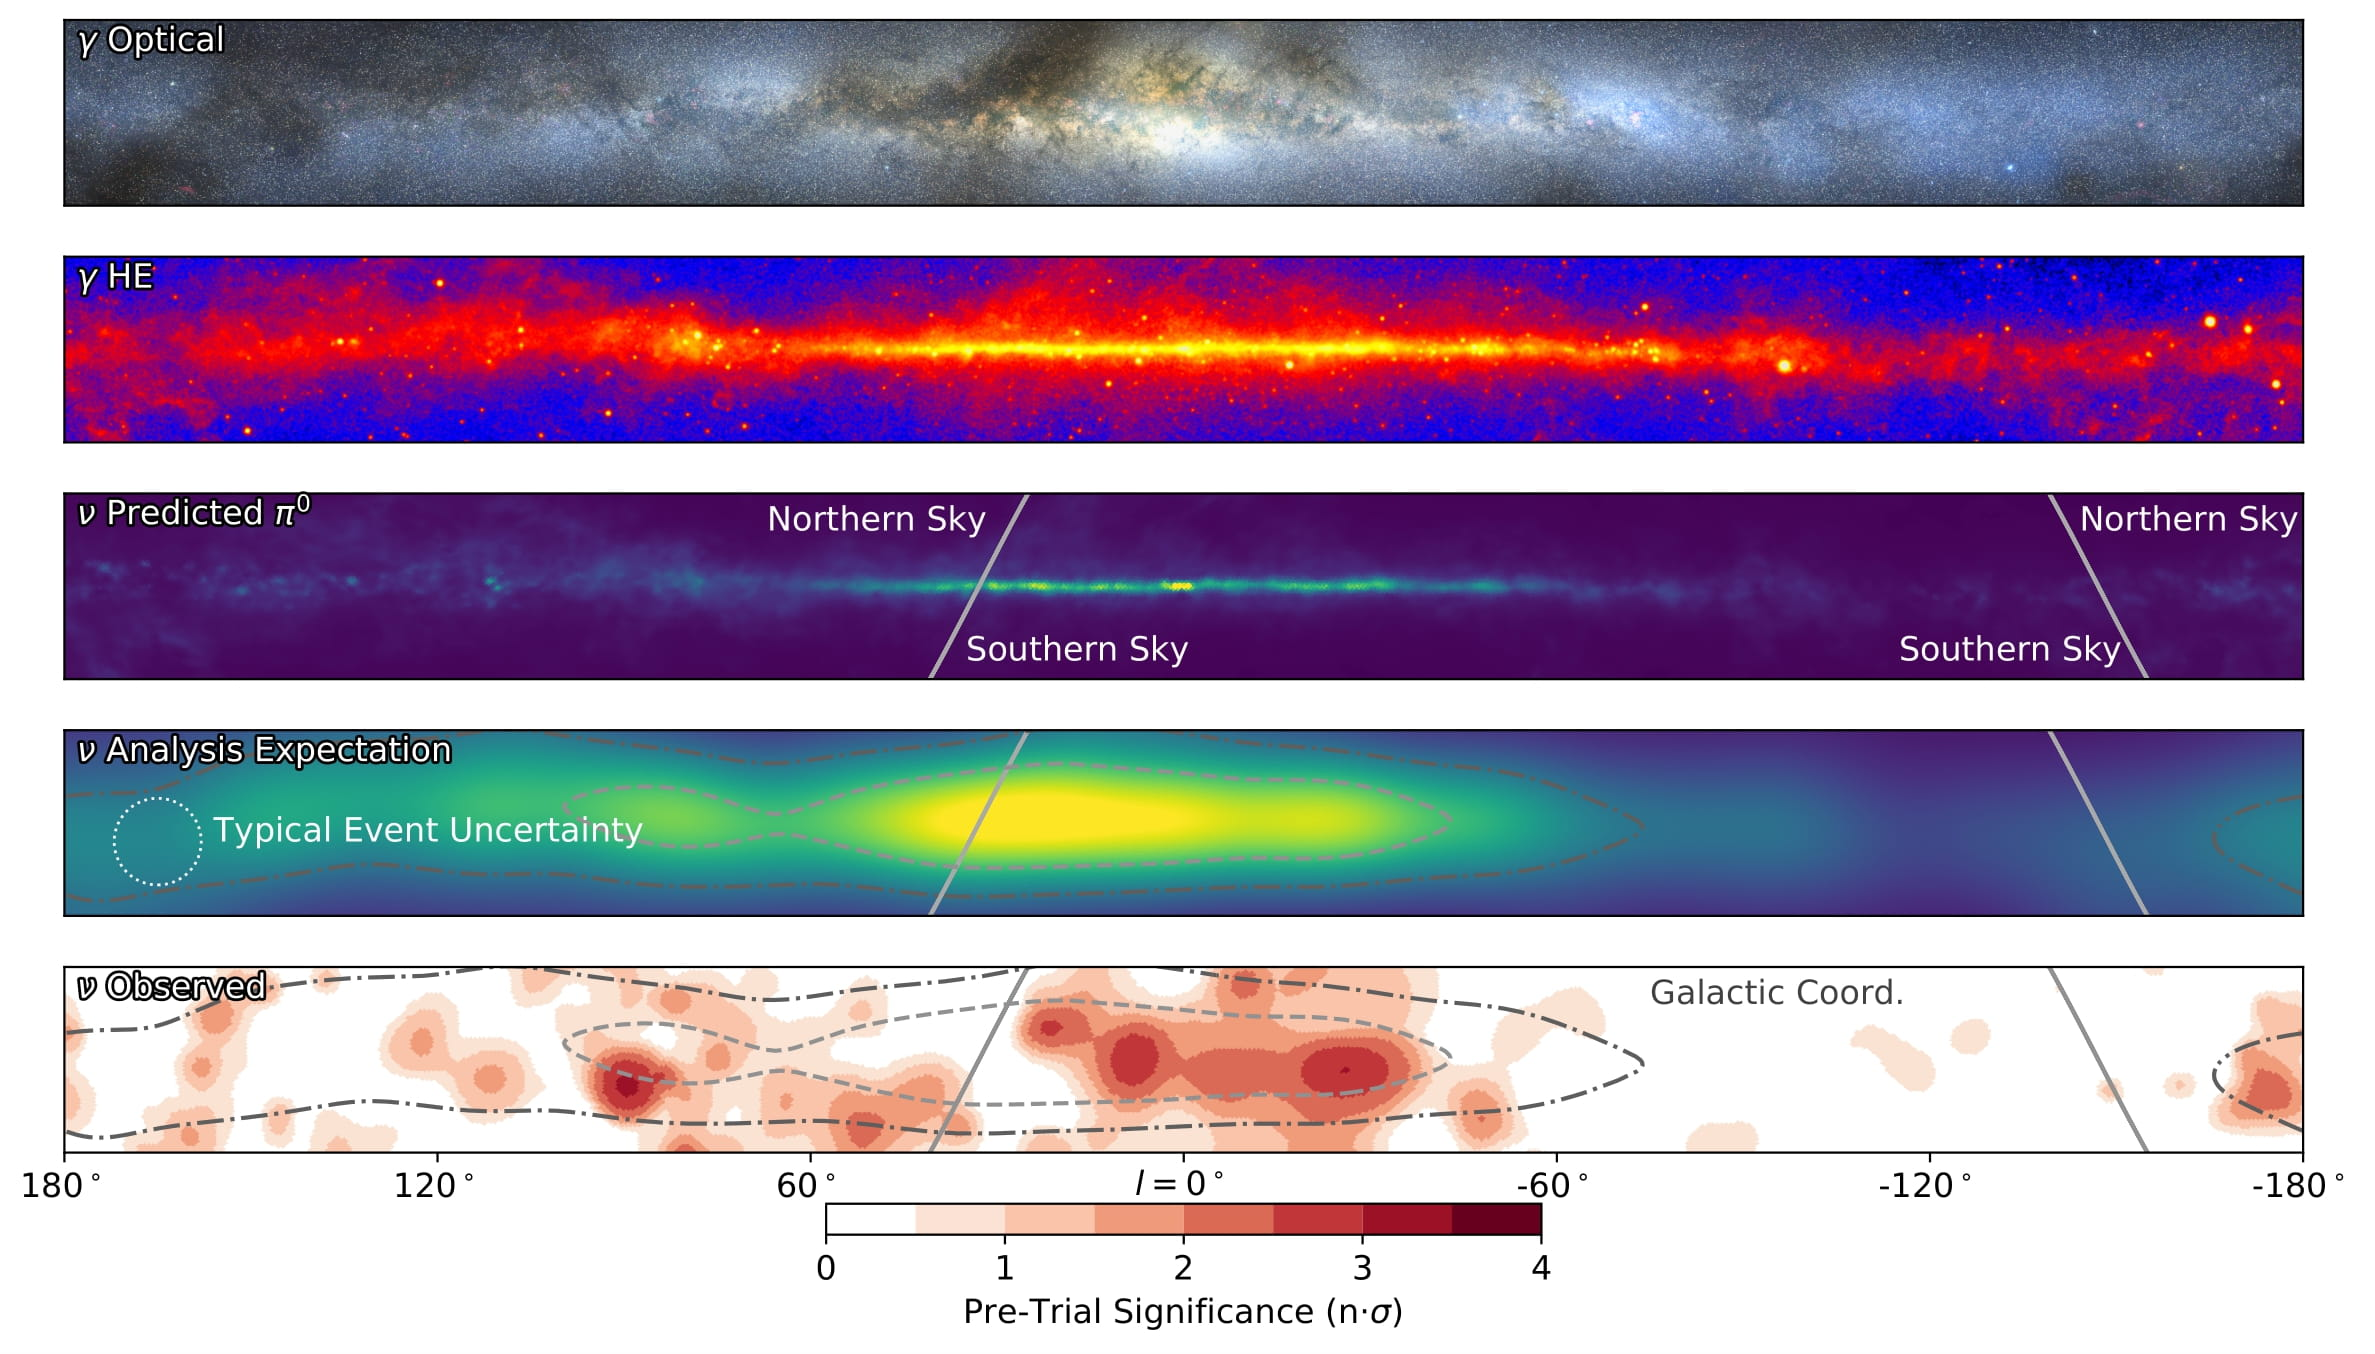
\includegraphics[scale=0.41]{figures/ic3_galacticplane.jpg}
        \caption{The Milky Way Galaxy in photons ($\gamma$) and neutrinos ($\nu$) \cite{2023:IC3_galactic_plane}. The Galactic center is at l = 0\textdegree and is the brightest region in all panels. (top) An Optical color image of the Milky Way galaxy seen from Earth. Clouds of gas and dust obscure some light from stars. (2nd down) Integrated flux of $\gamma$-rays observed by the Fermi-LAT telescope \cite{fermi:mw_plane}. (middle) Expected neutrino emission that corresponds with Fermi-LAT observations. (2nd up) Expected neutrino emission profile after considering detector systematics of IceCube. (bottom) Observed neutrino emission from region of the galactic plane. Substantial neutrino emission was detected.}
        \label{fig:ic3_mw}
    }
\end{figure}

The IceCube collaboration recently published a groundbreaking result of the Milky Way in neutrinos.
The recent result from IceCube, shown in \Cref{fig:ic3_mw}, proves that we can make observations under different messenger regimes.
The top two panels show the appearance of the galactic plane to different wavelengths of light.
Some sources are more apparent in some panels, while others are not.
This new channel is powerful because neutrinos are readily able to penetrate through gas and dust in the Milky Way.
This new image also refines our understanding of how high energy particles are produced.
For example, the fit to IceCube data prefers neutrino production from the decay of $\pi^0$ \cite{2023:IC3_galactic_plane}.

\begin{figure}[h]
    \centering{
        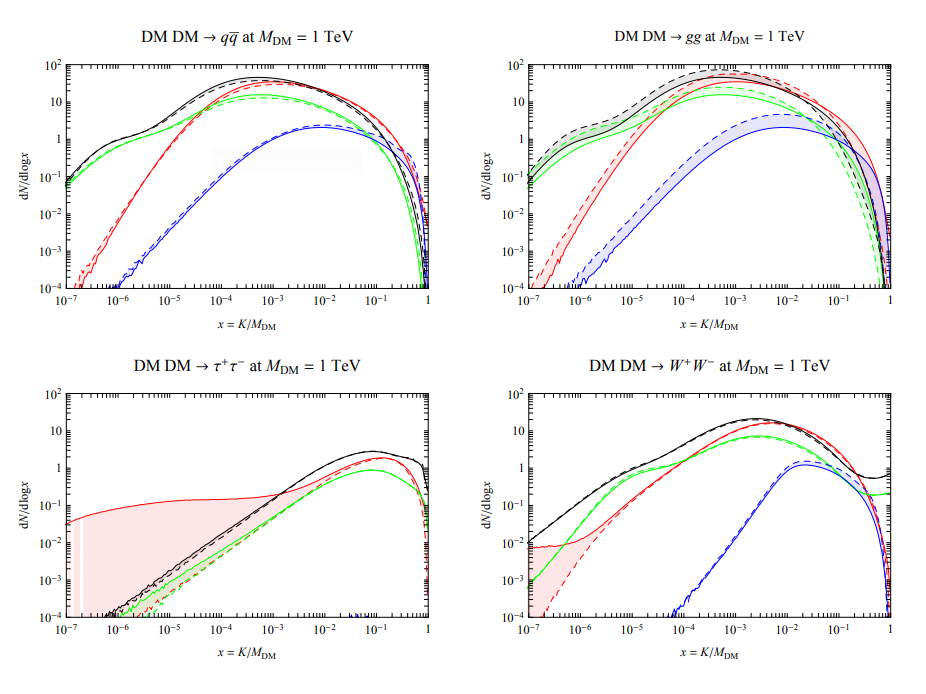
\includegraphics[scale=0.65]{figures/pppc_spectra.png}
        \caption{Dark Matter annihilation spectra for different final state particles and standard model annihilation channels \cite{pppc}. Photons (red), $e^\pm$ (green), $\bar{p}$ (blue), $\nu$ (black).}
        \label{fig:pppc_spectra}
    }
\end{figure}

Exposing our observations to more cosmic messengers greatly increases our sensitivity to rare processes.
In the case of DM, \Cref{fig:pppc_spectra},  there are many SM particles produced in DM annihilation.
Among the final state fluxes are gammas and neutrinos.
Charged particles are also produced however they would not likely make it to Earth since they will be deflected by magnetic fields between the source and Earth.
This means observatories that can see the neutral messengers are especially good for DM searches and for combining data for a multi-messenger DM search.


%%%%%%%%%%%%%%%%%%%%%%%%%%%%%%%%%%%%%%%%%%%%%%%%%%%%%%%%%%%%%%%%%%%%%%%%%%%%%%%%%%%%%
\chapter{Multimessenger Astrophysics: Detecting High Energy Neutral Messengers\label{sec:multmessenger}}
%%%%%%%%%%%%%%%%%%%%%%%%%%%%%%%%%%%%%%%%%%%%%%%%%%%%%%%%%%%%%%%%%%%%%%%%%%%%%%%%%%%%%
%-----------------------------------------------------------------------------------%
\section{Introduction\label{sec:chap3_intro}}
%-----------------------------------------------------------------------------------%

Before the 20th century, all asttrophysics observations were optical in nature.
We litterally only saw things with highly magnifiied optical observations.
Then we discovered cosmic rays.
cosmic rays are charged particles, typically naked protons or H+.
This was seen by Victor Hess in 19??.
Around the same time we discovered neutrinos from beta decay.
Sometime around 1950 we started to build neutrino detectors which were mostly sensitive to neutrinos from the sun.
Finally, it was theorized that compact objects like black holes and neutron stars would create waves in space-time when they experience mergers or collisions.

In the 21st century, we have developed new observation techniques and detectors that are no only sensitive to these four messengers - photons (\todo{photon}), neutrinos (\todo{nu}), Cosmic Rays (CR), and Gravitational Wave (WV) - we're collect high energy versions of these events.
For the standad model particles, we're now sensitive to all messengers above the MeV eneryg range.
Additionally, the GW's were sensitive to are in the stellar mass black hole region and above within our galactic neighborhood.
This means were becoming sensitive to the fundamental physics occuring within the universe and we can rely on the universe as a TeV+ particle accelerator.
We also have the abaility to correlate high energy events across messengers and gain new insights on the processes that occur in our universe.

This thesis focuses on very high energy (VHE) gamma rays and neutrinos.
These can both be observed through the water cherenkov detection technique altho not exclusively.
Methods on how to detect and observe these neutral messengers are discussed \cref{sec:mtm_gamma} and \cref{sec:mtm_nu}

%-----------------------------------------------------------------------------------%
\section{Charged Particles in a Medium\label{sec:cherenkov}}
%-----------------------------------------------------------------------------------%

For high enery gamma-rays and neutrinos, we can exploit the same effect that charged particles have with water.
This effect is known as Cherenkov radiation.
Cherenkov Radiation occurs when a charged particle, usually electrons ($e$) or muons ($\mu$), traverse a medium, like water, faster than the speed of light in that medium.
This is similar to sonic boom where an object moves through air faster than the speed of sound in air.
Cherenkov radiation can therefor be thought of as an 'optic boom'.
Many astro-particle physics experiments will use water as the medium as because water has a unique set of properties ideal for charged particle tracking.

\tmpfig{Show a nuclear reactor with cherenkov radiation}

The frequency of light emmited due to cherenkov radiation follows the equation:
\eqin{Cherenkov wavelength calc}
The absorption spectra is shown in the following figure:
\tmpfig{absorption spectrum of liquid and solid water}

%-----------------------------------------------------------------------------------%
\section{Photons ($\gamma$)\label{sec:mtm_gamma}}
%-----------------------------------------------------------------------------------%

%-----------------------------------------------------------------------------------%
\section{Neutrinos ($\nu$)\label{sec:mtm_nu}}
%-----------------------------------------------------------------------------------%

%-----------------------------------------------------------------------------------%
\section{Opportunities to Combine for Dark Matter\label{sec:ic3_hawc_combo}}
%-----------------------------------------------------------------------------------%


%%%%%%%%%%%%%%%%%%%%%%%%%%%%%%%%%%%%%%%%%%%%%%%%%%%%%%%%%%%%%%%%%%%%%%%%%%%%%%%%%%%%%
\chapter{High Altitude Water Cherenkov (HAWC) Observatory\label{sec:hawc}}
%%%%%%%%%%%%%%%%%%%%%%%%%%%%%%%%%%%%%%%%%%%%%%%%%%%%%%%%%%%%%%%%%%%%%%%%%%%%%%%%%%%%%
%-----------------------------------------------------------------------------------%
\section{The Detector}\label{sec:THE_hawc}
%-----------------------------------------------------------------------------------%

\begin{figure}[h!]
    \centering{
    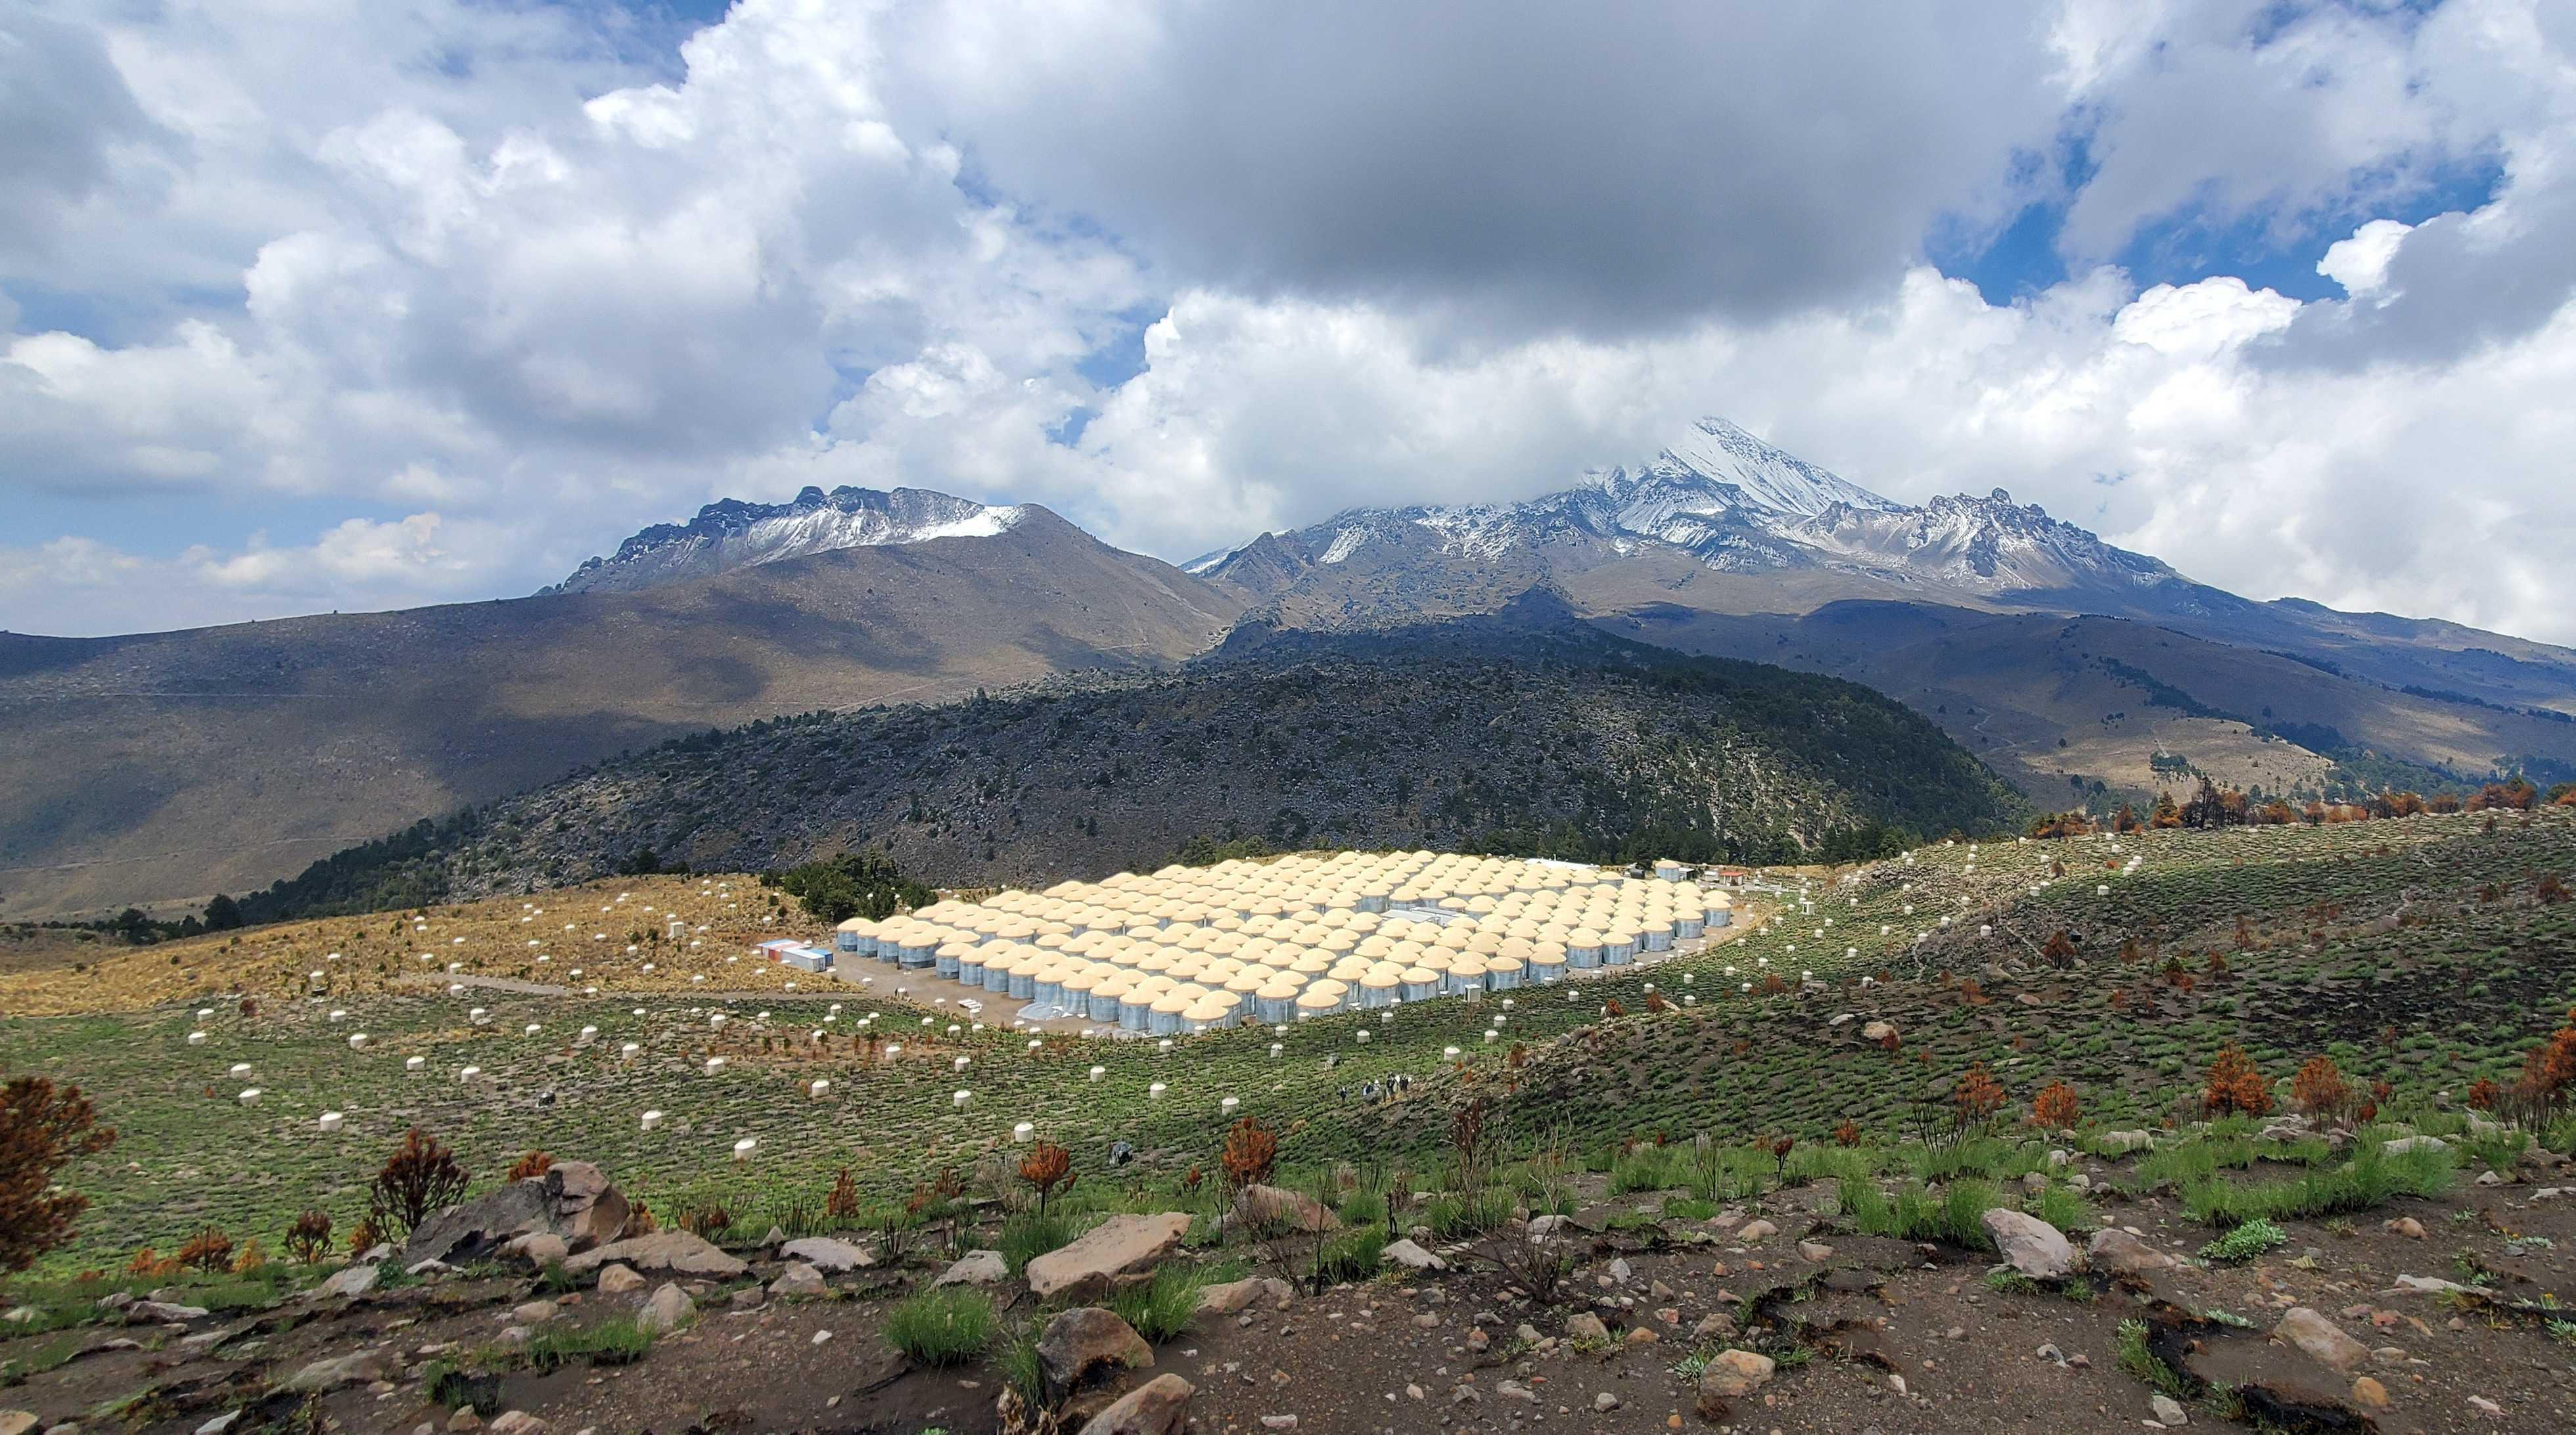
\includegraphics[scale=0.155]{figures/hawc/HAWC.jpg}
    }
    \caption{Photo of the HAWC detector that I took on May 17, 2023. Main array is centered in the photo and comprised of the larger tanks. Outriggers are the smaller tanks around the main array.}
    \label{fig:HAWC}
\end{figure}

The High Altitude Water Cherenkov (HAWC) Observatory is a specialized instrument designed for the observation of high energy gamma-rays and cosmic rays \cite{HAWC_NIM}.
Located on the Sierra Negra volcano in Mexico, HAWC observes gamma rays and cosmic rays in the energy range of approximately 100 GeV to 100's of TeV.
HAWC is strategically situated to maximize observational efficiency due to its high altitude.
At an elevation of 4,100 meters, it monitors about two-thirds of the sky every day with an uptime above 90\%.
This capability is essential for studying high-energy astrophysical phenomena.

HAWC consists of 300 water Cherenkov detectors (WCDs) spread over 22,000 $m^2$.
Each main array detector is filled with purified water and equipped with four, upward-facing photomultiplier tubes (PMTs).
See \cref{fig:WCD_schematic} for schematic of WCDs.
These PMTs detect Cherenkov radiation from charged particles passing through the tanks.
These charged particles are generated when a high energy gamma or cosmic ray collides with gas in the atmosphere to create a charged particle shower, see \cref{fig:airshowers}.
The observatory includes a separate tank configuration which are refered to as the outriggers.
They are a secondary array of 345 smaller WCD's.
Surrounding the main array, each outrigger tank measures 1.55 meters in diameter and height and contain a single upward-facing eight-inch PMT.
This add-on increases the instrumented footprint fourfold.
The outriggers are meant to improve the reconstruction of showers extending beyond the main array, especially for events above 10 TeV.
However, at the time of writing this thesis, the outriggers have not been fully integrated into HAWC's reconstruction software.

\begin{figure}
    \centering{
    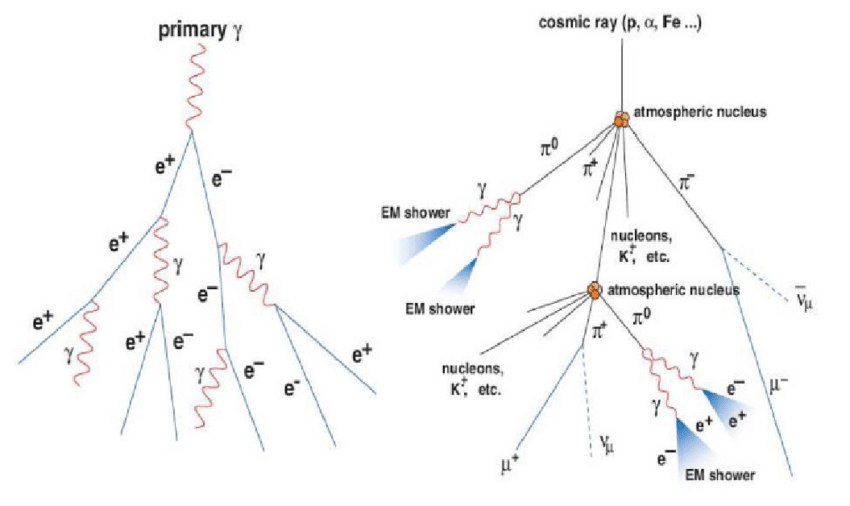
\includegraphics[scale=0.5]{figures/hawc/high_energy_air_shower.png}
    }
    \caption{A particle physics illustration of high energy particle showers. Left shower is an electromagnetic shower from a high energy gamma-ray. Most particles in the shower will be a combination of photons and charged leptons, in this case electrons (e). Right figure shows a cosmic ray particle shower. The cosmic ray will produce many more types of particles including pions ($\pi$), neutrinos, and charged leptons. Figured pulled from \cite{lopez_thesis}.}
    \label{fig:airshowers}
\end{figure}

%-----------------------------------------------------------------------------------%
\subsection{Construction and Hardware} \label{sec:hawc_hardware}
%-----------------------------------------------------------------------------------%

\begin{figure}
    \centering{
        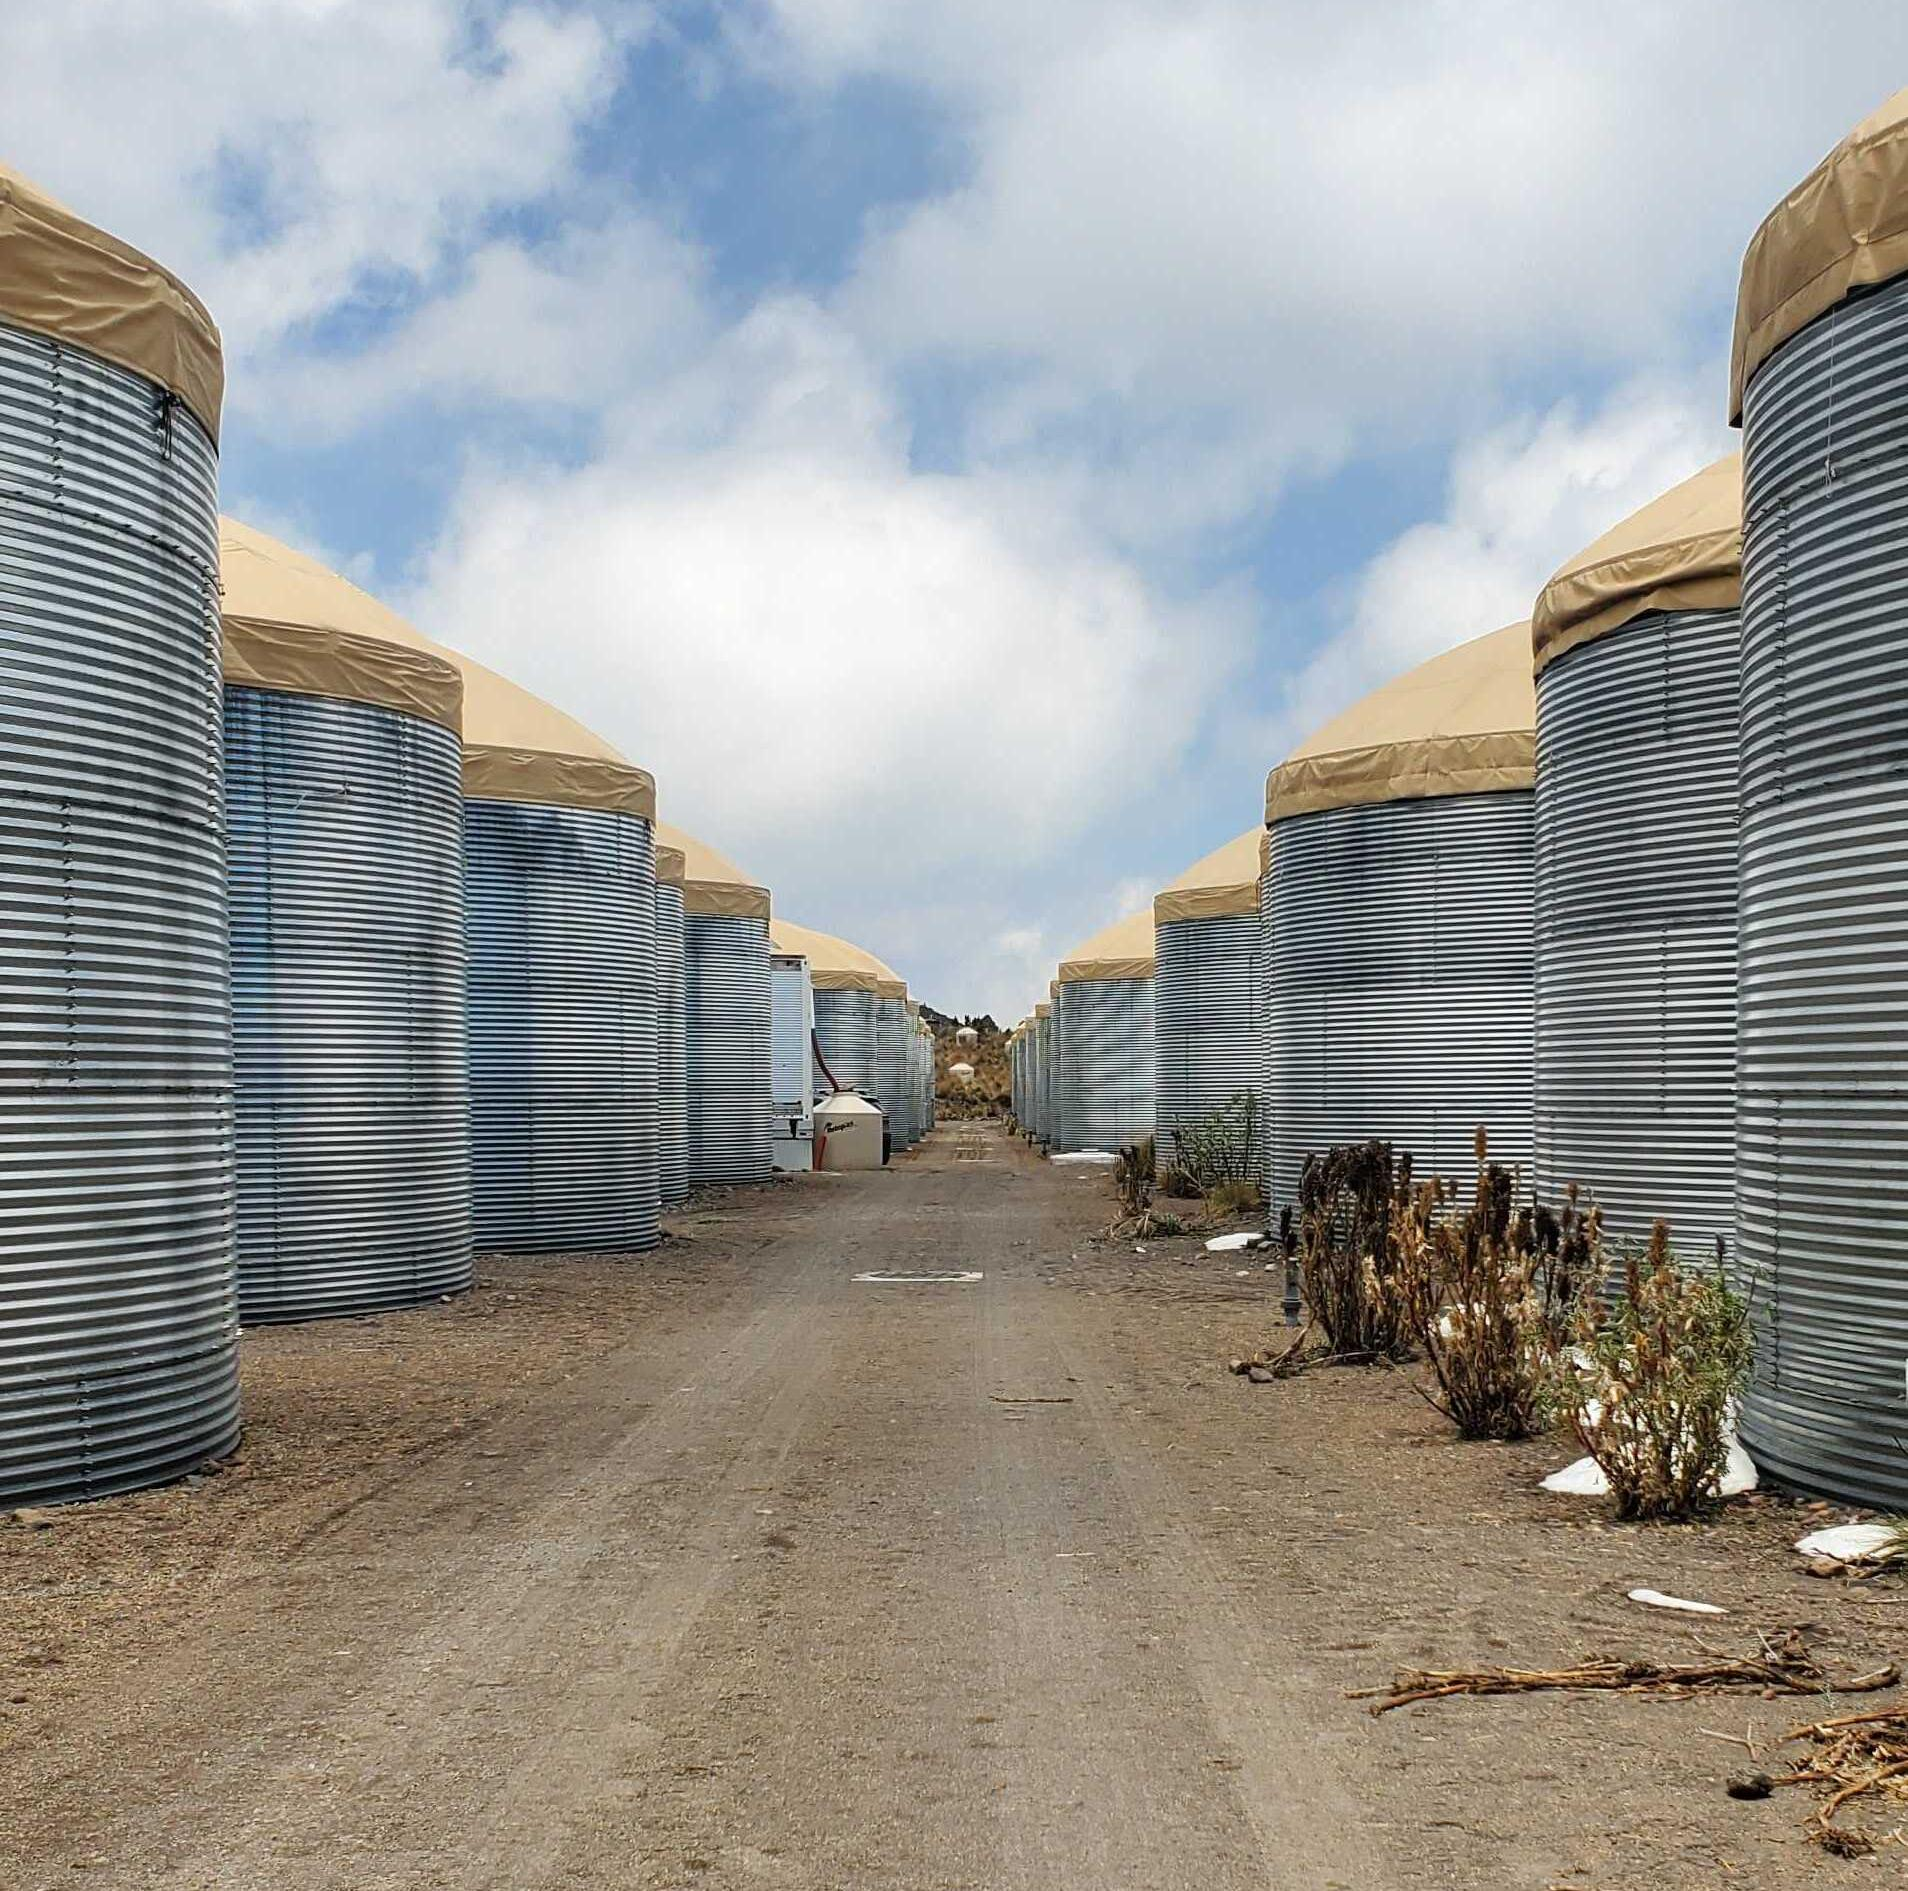
\includegraphics[scale=0.14]{figures/hawc/WCDs.jpg}
        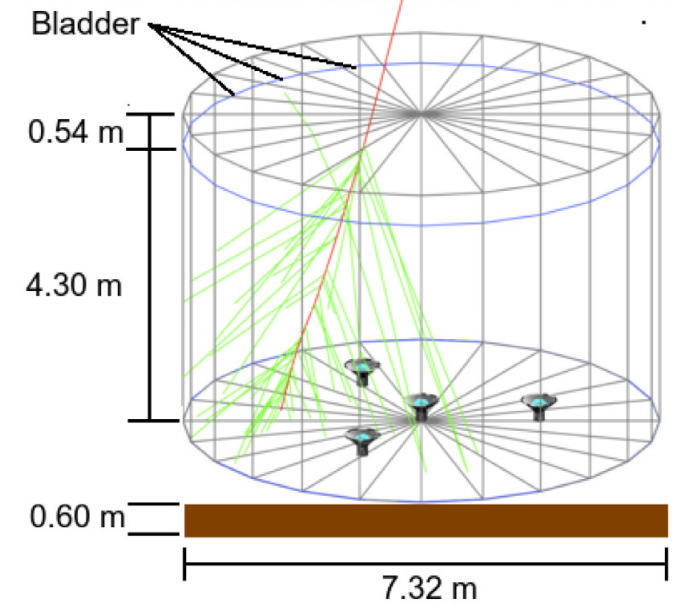
\includegraphics[scale=0.45]{figures/hawc/WCD_schematic.png}
    }
    \caption{The WCDs. Left image features several WCDs looking from within the main array of HAWC. Right image shows a schematic of a WCD pulled from \cite{HAWC_NIM}.}
    \label{fig:WCD_schematic}
\end{figure}

Each main array WCD, see \cref{fig:WCD_schematic}, is a cylindrical tank with dimensions of 7.3 m in diameter and 5.4 m in height and filled with 180,000 L of water \cite{HAWC_NIM}.
The metal shell of these tanks is made from bolted together, corrugated, galvanized steel panels.
The tanks are placed into 0.6 m deep trenches filled with rammed earth to secure it against seismic activity \cite{HAWC_NIM}.
The interior of each tank is lined with a black, low-density polyethylene bladder, designed to be impermeable to external light and to prevent reflection of Cherenkov light within the tank.
This bladder is approximately 0.4 mm thick and composed of two layers of three-substrate film.
To further minimize light penetration, a black agricultural foil covers the bladder.
The ground and walls inside the tank are protected with felt and sand to safeguard against punctures.
The tanks are filled 4.5 m deep of purified water, achieving a photon attenuation length for Cherenkov photons that exceeds the tank's dimensions \cite{HAWC_NIM}.
This purification level ensures the optimal detection environment for the photons generated by traversing charged particles.

At the base of each tank, four photomultiplier tubes (PMTs) are installed to detect the Cherenkov radiation emitted by charged particles in watre.
Three 8-inch diameter PMTs surround a larger 10 inch PMT from Hamamatsu \cite{hawc_pmt}.
The variation in PMT response is carefully accounted for in event reconstruction algorithms.
Signals from the PMTs traverse 610 ft cables to the counting house, where they are processed by Front-End Boards (FEBs), see \cref{fig:basic_tanks_schem,fig:dig_schem}.
These FEBs, along with Time to Digital Converters (TDCs), digitize the signals and manage the high voltage supply to the PMTs.

%-----------------------------------------------------------------------------------%
\subsection{Data Acquisition and Signal Processing} \label{sec:hawc_daq}
%-----------------------------------------------------------------------------------%

\begin{figure}
    \centering{
        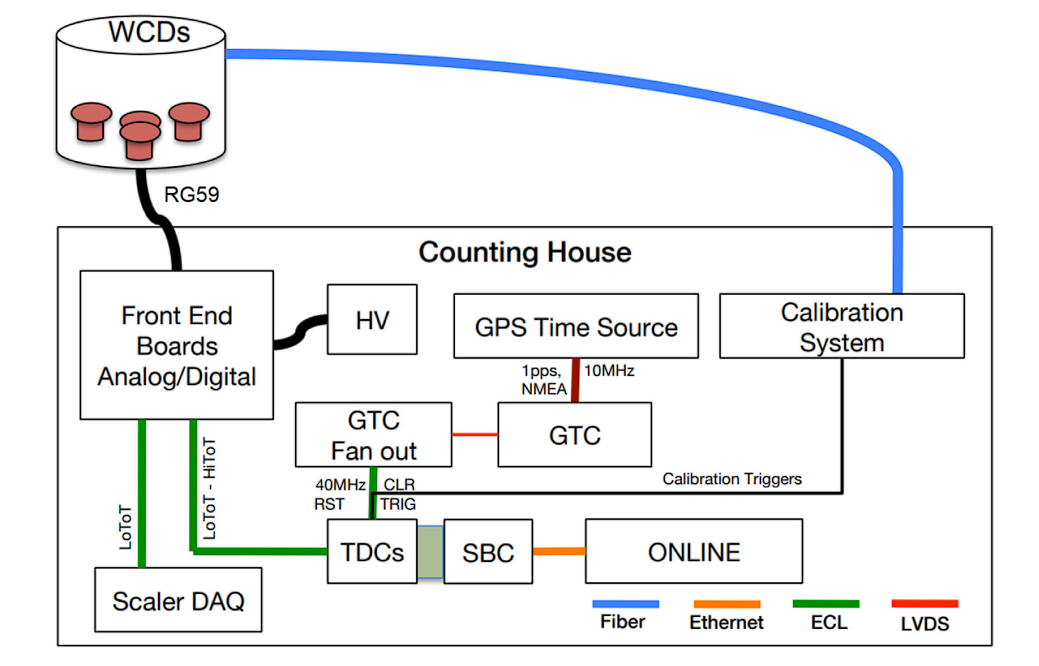
\includegraphics[scale=0.5]{figures/hawc/tank_basic_schem.png}
    }
    \caption{Overview of HAWC control and data electronics. The LoToT and HiToT threshold signals are discussed in \cref{sec:hawc_daq}. Figure from \cite{HAWC_NIM}}
    \label{fig:basic_tanks_schem}
\end{figure}

\begin{figure}
    \centering{
        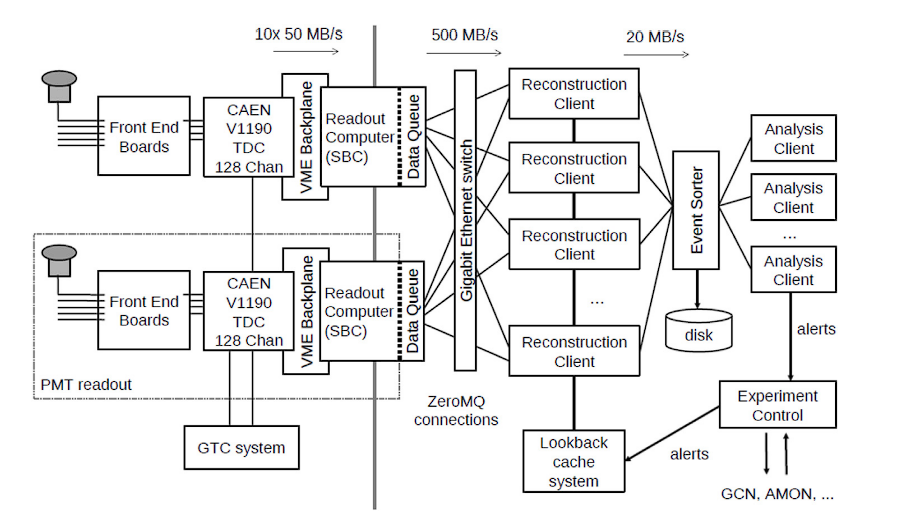
\includegraphics[scale=0.6]{figures/hawc/digital_schematic.png}
    }
    \caption{Schematic of data flow in HAWC data acquisition and online processing system. Pulled from \cite{HAWC_DAQ_NIM}.}
    \label{fig:dig_schem}
\end{figure}

The HAWC data acquisition (DAQ) and signal processing systems convert the physical detection of particles into analyzable data.
This process involves a series of steps from initial signal detection by PMTs to digital conversion and preliminary analysis, see \cref{fig:dig_schem,fig:tot_threholds}.

\begin{figure}
    \centering{
        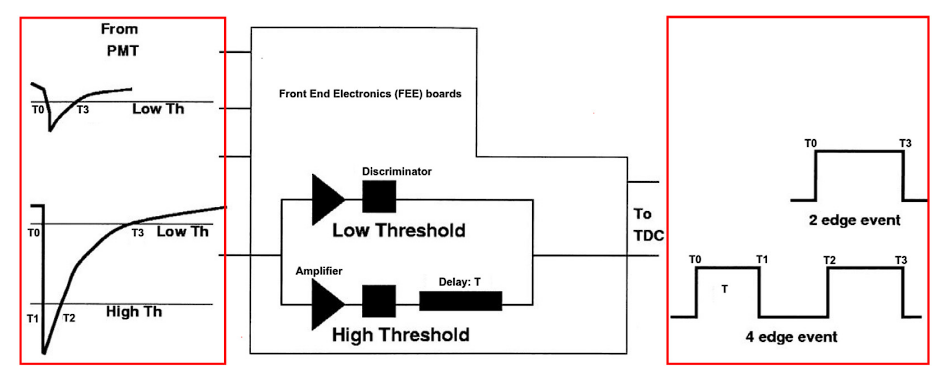
\includegraphics[scale=0.6]{figures/hawc/ToT_threshold.png}
    }
    \caption{How HAWC FEB intially processes analog PMT signals. Signals are split through an amplifier and discriminator circuit. Each path is designated for either the HIGH or LOW threshold for the signal. The 2-edge event corresponds to LOW, while the 4 edge corresponds to HIGH.}
    \label{fig:tot_threholds}
\end{figure}

Once the signal from the PMTs arrive at the counting house, they enter the Front-End Boards (FEBs).
The FEBs are responsible for the initial processing of these signals, which includes amplification and integration \cite{Milagro_DAQ}.
Each PMT signal is compared against preset LOW/HIGH voltage thresholds in the FEBs, see \cref{fig:tot_threholds}, identifying signals that correspond to about 1/4 and 4 photoelectrons, respectively.
This differentiation allows the system to gauge the strength of the detected Cherenkov radiation.
The processed signals are then digitized by Time to Digital Converters (TDCs).
These converters measure the time over threshold (ToT) for each signal, a parameter that reflects both the duration and amplitude of the signal.
This digitization facilitates reconstruction of the original event for translating the physical interactions within the detectors into data \cite{HHAWC_NIM,HAWC_DAQ_NIM,Milagro_DAQ}.

Synchronization across the HAWC observatory is maintained by a central GPS Timing and Control (GTC) system, which achieves a timing resolution of 98 ps.
This high-resolution timing is vital for accurately reconstructing the timing and location of air showers initiated by cosmic and gamma rays.
The GTC system ensures that all components of the DAQ operate in unison to preserve the temporal integrity of the detected events \cite{HHAWC_NIM,hawc_daq_thesis}.

Once digitized, the data are transferred to an online event reconstruction system.
This system runs the Reconstruction Client, which utilizes the raw PMT data to reconstruct the characteristics of the air showers, such as their direction and energy \cite{HAWC_DAQ_NIM}.
The capacity for real-time analysis allows HAWC to promptly respond to astrophysical phenomena like Gamma Ray Bursts (GRBs) and to participate in multi-messenger astronomy by following up on alerts from other observatories.
This real-time processing system is designed to handle high data throughput, using ZeroMQ \cite{zeromq} for efficient data transfer between software components.
Analysis Clients perform specific online analyses that require immediate data, including monitoring for GRBs, solar flare activity, and participation in global efforts to track gravitational waves and neutrinos \cite{HAWC_NIM}.

The DAQ system is overseen by an Experiment Control system and crew that manage the operational aspects of data collection.
This includes initiating and terminating data collection runs and monitoring the experiment for errors.
In the event of a system crash, often caused by environmental factors such as lightning, the Experiment Control system is designed to automatically restart the experiment and minimize downtime \cite{HAWC_NHAWC_NIM,HAWC_DAQ_NIM}.

%-----------------------------------------------------------------------------------%
\section{Event Reconstruction} \label{sec:hawc_reconstruction}
%-----------------------------------------------------------------------------------%

Event reconstruction at the HAWC Observatory is a critical procedure that converts the raw data from the observatory's WCDs into a coherent framework for understanding cosmic and gamma-ray events.
This process includes several distinct steps.
Core Fitting determines the geometric center of the air shower on the detector plane.
Angle Reconstruction assesses the trajectory of the incoming particle, revealing its origin in the sky.
Energy Estimation is performed using both \textit{f}-hit and Neural Network (NN) methods to quantify the energy of the detected events.
Gamma/Hadron discrimination differentiates between gamma-ray and hadronic cosmic ray initiated showers, a vital step for astrophysical interpretations.
Each of these steps is integral to the observatory's objective of investigating the high-energy universe and enable the transformation of signals into detailed insights about high energy cosmic phenomena.

%$$$$$$$$$$$$$$$$$$$$$$$$$$$$$$$$$$$$$$$$$$$$$$$$$$$$$$$$$$$$$$$$$$$$$$$$$$$$$$$$$$$%
\subsection{Core Fitting} \label{sec:hawc_core_fitting}
%$$$$$$$$$$$$$$$$$$$$$$$$$$$$$$$$$$$$$$$$$$$$$$$$$$$$$$$$$$$$$$$$$$$$$$$$$$$$$$$$$$$%

\begin{figure}[h!]
    \centering{
    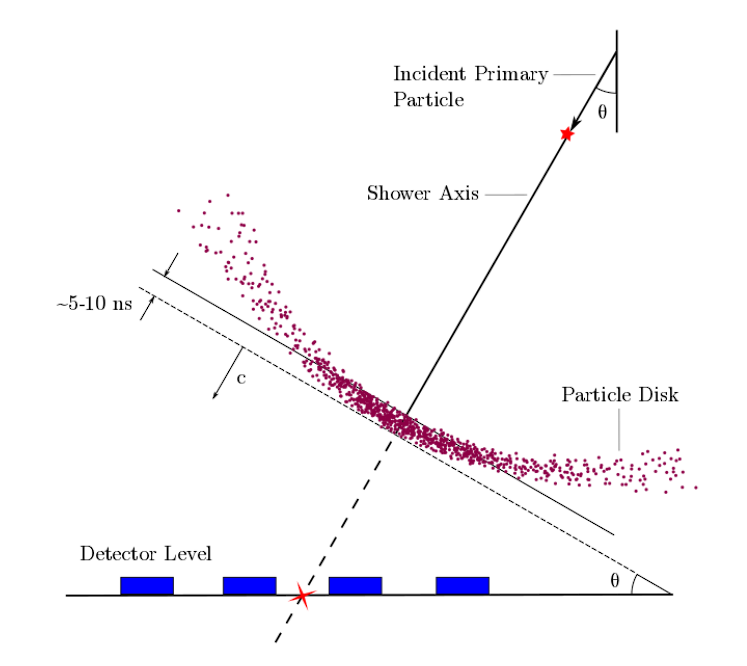
\includegraphics[scale=0.5]{figures/hawc/shower_shape.png}
    }
    \caption{An particle shower incident on WCDs. Secondary particles of an air shower travel in a cone centered on primary incident particle. Reconstruction of the initial angle is possible with arrival time of hits in PMTs inside WCDs. Figure from \cite{thesis_Zigg}.}
    \label{fig:shower_shape}
\end{figure}

In the study of air showers, accurately determining the location of the air shower core on the ground is crucial for reconstructing the direction of the originating primary particle.
An illustration of this can be seen in a HAWC event plot, \cref{fig:airshowers,fig:ldf_particleshower}, where the lateral charge distribution across the array is displayed.
The core is identified and marked with a red star, reconstructed using a predetermined functional form, \cref{eq:hawc_showercore}.

We model signal $S_i$ from the \textit{i}th PMT is given by the following equation:
\showercore
In this model, $\tilde{x}$ represents the core location and $\tilde{x}_i$ is the position of the \textit{i}th PMT.
$R_m$ stands for the Molière radius, which is approximately 120 meters at the altitude of HAWC.
$\sigma$ is the standard deviation of the Gaussian distribution.
$N$ is the normalization factor for the tail of the distribution.
The equation incorporates fixed values of $\sigma = 10$ m and $N=5.10^{-5}$.
This leaves the core location and overall amplitude $A$ as the free parameters to be determined during fitting.

\begin{figure}
    \centering{
        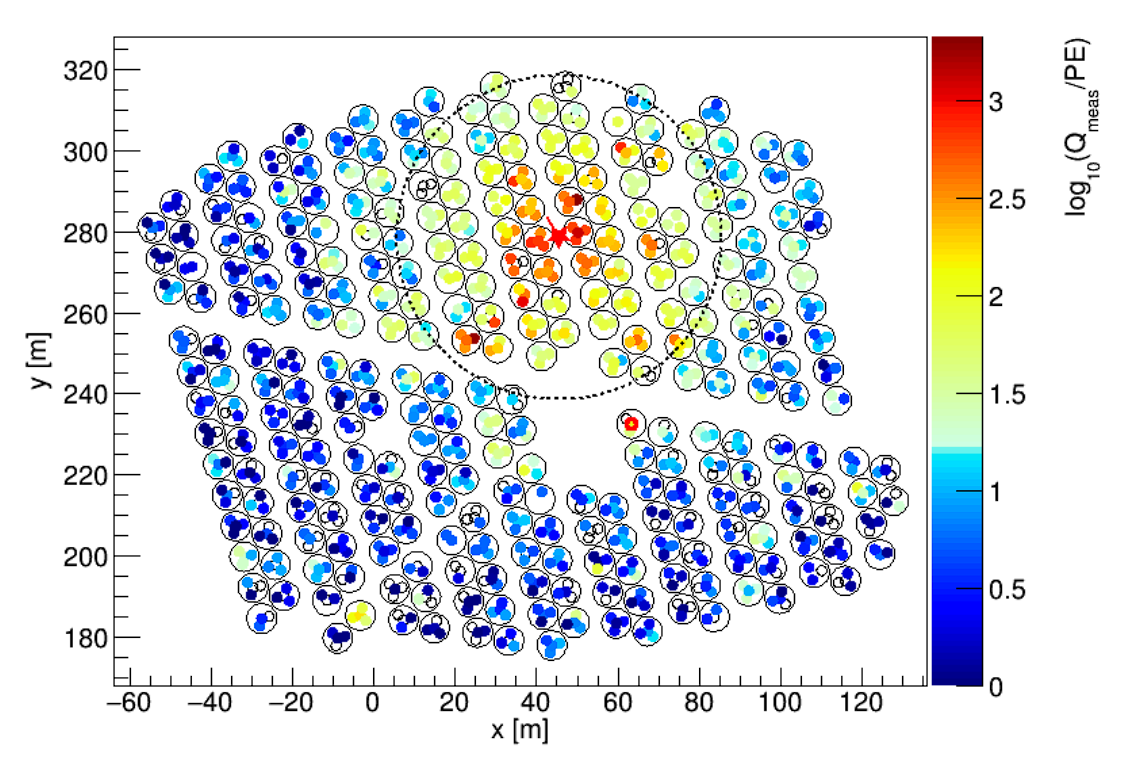
\includegraphics[scale=0.5]{figures/hawc/core_fitting.png}
    }
    \caption{Charge deposition in each PMT for a reconstructed gamma-ray event. WCDs are outlined in black surrounding the 4 smaller circles that represent PMTs. The color scale indicates the charge deposition in each PMT. The best shower core fit from SFCF is noted with a red star in the center of the dashed circle \cite{Abeysekara_2017}.}
    \label{fig:core_fitter}
\end{figure}

The chosen functional form for the Super Fast Core Fit (SFCF) algorithm is a simplified version of a modified Nishimura-Kamata-Greisen (NKG) function \cite{cosmic_ray_shape}, selected for its computational efficiency which is essential for rapid fitting of air shower cores.
The SFCF form allows numerical minimization to converge more quickly due to the function's simplicity, the analytical computation of its derivatives, and the absence of a pole at the core location \cite{Abeysekara_2017}.
\Cref{fig:core_fitter} provides a visualization of a recorded event, with the plot depicting the charge recorded by each PMT as a function of the distance to the reconstructed shower core.
Through the application of the SFCF, core locations can be identified with a median error of approximately 2 m for large events and about 4 m for smaller ones, assuming the gamma-ray event core impacts directly upon the HAWC detector array \cite{Abeysekara_2017}.
It is noted that as the core's distance from the main array increases, the precision in locating the core diminishes \cite{Abeysekara_2017}, highlighting the importance of proximity in the accuracy of core reconstruction.


%$$$$$$$$$$$$$$$$$$$$$$$$$$$$$$$$$$$$$$$$$$$$$$$$$$$$$$$$$$$$$$$$$$$$$$$$$$$$$$$$$$$%
\subsection{Angle Reconstruction} \label{sec:hawc_angleReco}
%$$$$$$$$$$$$$$$$$$$$$$$$$$$$$$$$$$$$$$$$$$$$$$$$$$$$$$$$$$$$$$$$$$$$$$$$$$$$$$$$$$$%

After establishing the core position, the next step is angle reconstruction.
This process determines the primary particle's trajectory.
The angle of arrival is indicative of the originating gamma ray's direction.
It correlates to the cosmic source of the gamma-ray.
We deduce this angle using the timing of PMT hits \cite{Abeysekara_2017}.

The air shower's front is conically shaped, not flat.
This shape arises from the travel patterns of secondary particles.
An event example is illustrated in \cref{fig:shower_shape}.
Far from the core, secondary particles undergo multiple scattering.
They also travel longer distances \cite{wcd_Sensitivity}.
Particle sampling decreases with distance from the core.
This decrease results in measurable delays in arrival times \cite{wcd_Sensitivity,Abeysekara_2017}.
Simulations provide a corrective measure for these effects.
The correction is a function of shower parameters \cite{Abeysekara_2017}.
It adjusts both curvature and sampling.
The distance from the shower core and the charge recorded by PMTs are crucial to this correction.
A function based on simulation and Crab Nebula observations is used for this purpose \cite{Abeysekara_2017}.
This curvature correction allows us to fit the particle front as a plane wave.

Corrections lead to the $\chi^2$ minimization step.
This technique fits a plane to the timing data of the PMTs.
It then calculates the shower's angle of arrival.
The zenith and azimuth angles are the results of this fit \cite{wcd_Sensitivity}.
The local angles are converted to celestial coordinates.
These coordinates allow correlation with gamma-ray sources.
Right ascension (RA) and declination (Dec) are used for this purpose.
RA is akin to longitude, and Dec to latitude.

The reconstructed angle's resolution ranges from 0.1° to 1°.
This range depends on the incoming particle's energy and zenith angle \cite{wcd_Sensitivity}.
The analysis uses a curvature/sampling correction.
This correction applies a quadratic function based on distance from the core \cite{Abeysekara_2017}.
The adjustment improves angular resolution.
However, discrepancies between simulation and observation persist.
These discrepancies introduce systematic errors into HAWC analyses \cite{Abeysekara_2017}.

%$$$$$$$$$$$$$$$$$$$$$$$$$$$$$$$$$$$$$$$$$$$$$$$$$$$$$$$$$$$$$$$$$$$$$$$$$$$$$$$$$$$%
\subsection{$f_\mathrm{hit}$ Energy Estimation}\label{sec:hawc_fhit}
%$$$$$$$$$$$$$$$$$$$$$$$$$$$$$$$$$$$$$$$$$$$$$$$$$$$$$$$$$$$$$$$$$$$$$$$$$$$$$$$$$$$%

\begin{figure}
    \centering{
        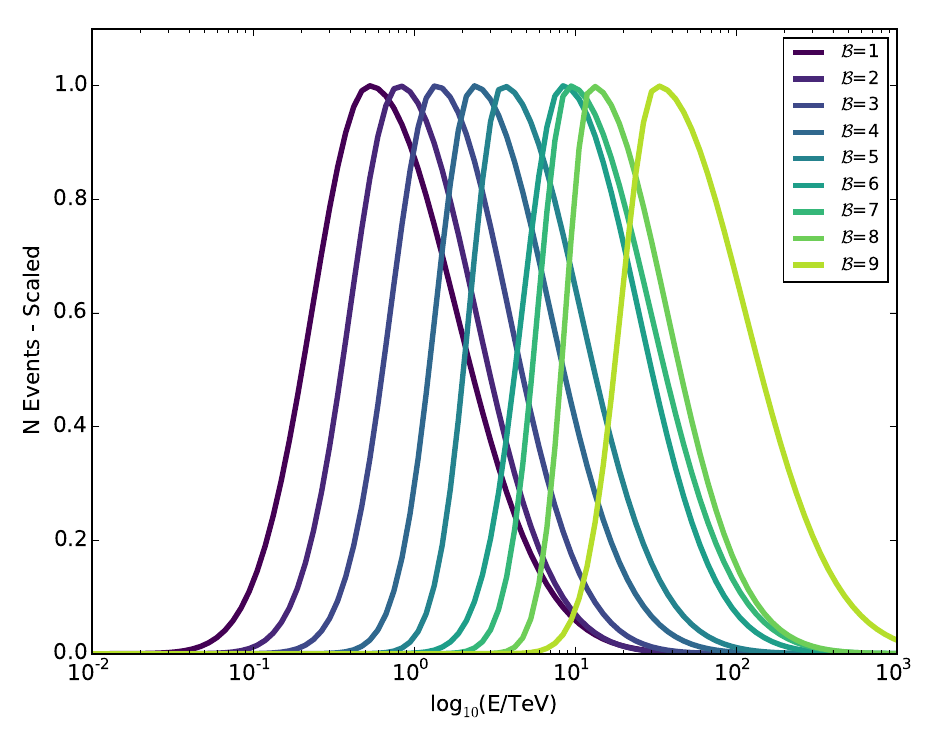
\includegraphics[scale=0.6]{figures/hawc/fhit_bins.png}
    }
    \caption{Simulated normalized energy distribution of each $f_\mathrm{hit}$ bin defined in \cref{tab:fhit_bins}. Monte Carlo simulation of gamma-rays with $E^-{2.63}$ spectral shape and simulated source at 20$^\circ$ declination. Figure from \cite{Abeysekara_2017}.}
    \label{fig:fhit_bins}
\end{figure}

\begin{table}
    \centering{
    \begin{tabular}{c?cc|c}
        \hline
        Bin &
        Lower Edge \% &
        Upper Edge \% &
        $\Theta_{68}$ ($^\circ$) \\
        \hline
        1       &
        6.7     &
        10.5    &
        1.05    \\

        2       &
        10.5    &
        16.2    &
        0.69    \\

        3       &
        16.2     &
        24.7    &
        0.50    \\

        4       &
        24.7     &
        35.6    &
        0.39    \\

        5       &
        35.6     &
        48.5    &
        0.30    \\

        6       &
        48.5     &
        61.8    &
        0.28    \\

        7       &
        61.8     &
        74.0    &
        0.22    \\

        8       &
        74.0     &
        84.0    &
        0.20    \\

        9       &
        84.0     &
        100    &
        0.17    \\

    \end{tabular}
    }
    \caption{Definitions of $f_\mathrm{hit}$ energy estimator bins. Bins are defined by the fraction of available PMTs that are triggered during an air shower event. The angular resolution, $\Theta_{68}$, is the bin containing 68\% of events \cite{Abeysekara_2017}.}
    \label{tab:fhit_bins}
\end{table}

The HAWC Observatory quantifies the primary particle energy of air showers using a metric known as $f_{\text{hit}}$.
This ratio compares the count of PMTs involved in the event reconstruction to the total number of functional PMTs at the time \cite{Abeysekara_2017}.
The main array consists of about 1200 PMTs, but the count may vary due to maintenance or other operational factors.

Events are stratified into several $f_{\text{hit}}$ bins.
Each bin corresponds to a specific range of angular resolutions, enabling a structured approach to event analysis based on the extent of the shower footprint, see \cref{tab:fhit_bins}.
The $f_{\text{hit}}$ metric, while effective, has several limitations.
It is dependent on the zenith angle and the spectral characteristics presumed for the observed source.
The variable also reaches a saturation point around 10 TeV, after which the detector's ability to discriminate between higher energy levels diminishes \cite{Abeysekara_2017}.
Furthermore, the energy distribution for each $f_{\text{hit}}$ bin is notably broad, see \cref{fig:fhit_bins}.
In response to these limitations, HAWC has developed more intricate algorithms for energy estimation.
These algorithms incorporate the zenith angle and the distribution of charge around the shower core for a more accurate assessment of the primary particle's energy, particularly at energies surpassing 10 TeV \cite{wcd_Sensitivity}.

The relationship between $f_{\text{hit}}$ and primary energy is complex.
Atmospheric attenuation can cause high-energy showers to present a smaller footprint, misrepresenting their energy in the $f_{\text{hit}}$ metric.
This effect is captured in simulations that chart the actual energy distribution across $f_{\text{hit}}$ categories \cite{wcd_Sensitivity}.
Such distributions vary with the declination of the source and the theoretical energy spectrum used in the model.

%$$$$$$$$$$$$$$$$$$$$$$$$$$$$$$$$$$$$$$$$$$$$$$$$$$$$$$$$$$$$$$$$$$$$$$$$$$$$$$$$$$$%
\subsection{Neural Network Energy Estimation}\label{sec:hawc_nn}
%$$$$$$$$$$$$$$$$$$$$$$$$$$$$$$$$$$$$$$$$$$$$$$$$$$$$$$$$$$$$$$$$$$$$$$$$$$$$$$$$$$$%

\begin{figure}
    \centering{
        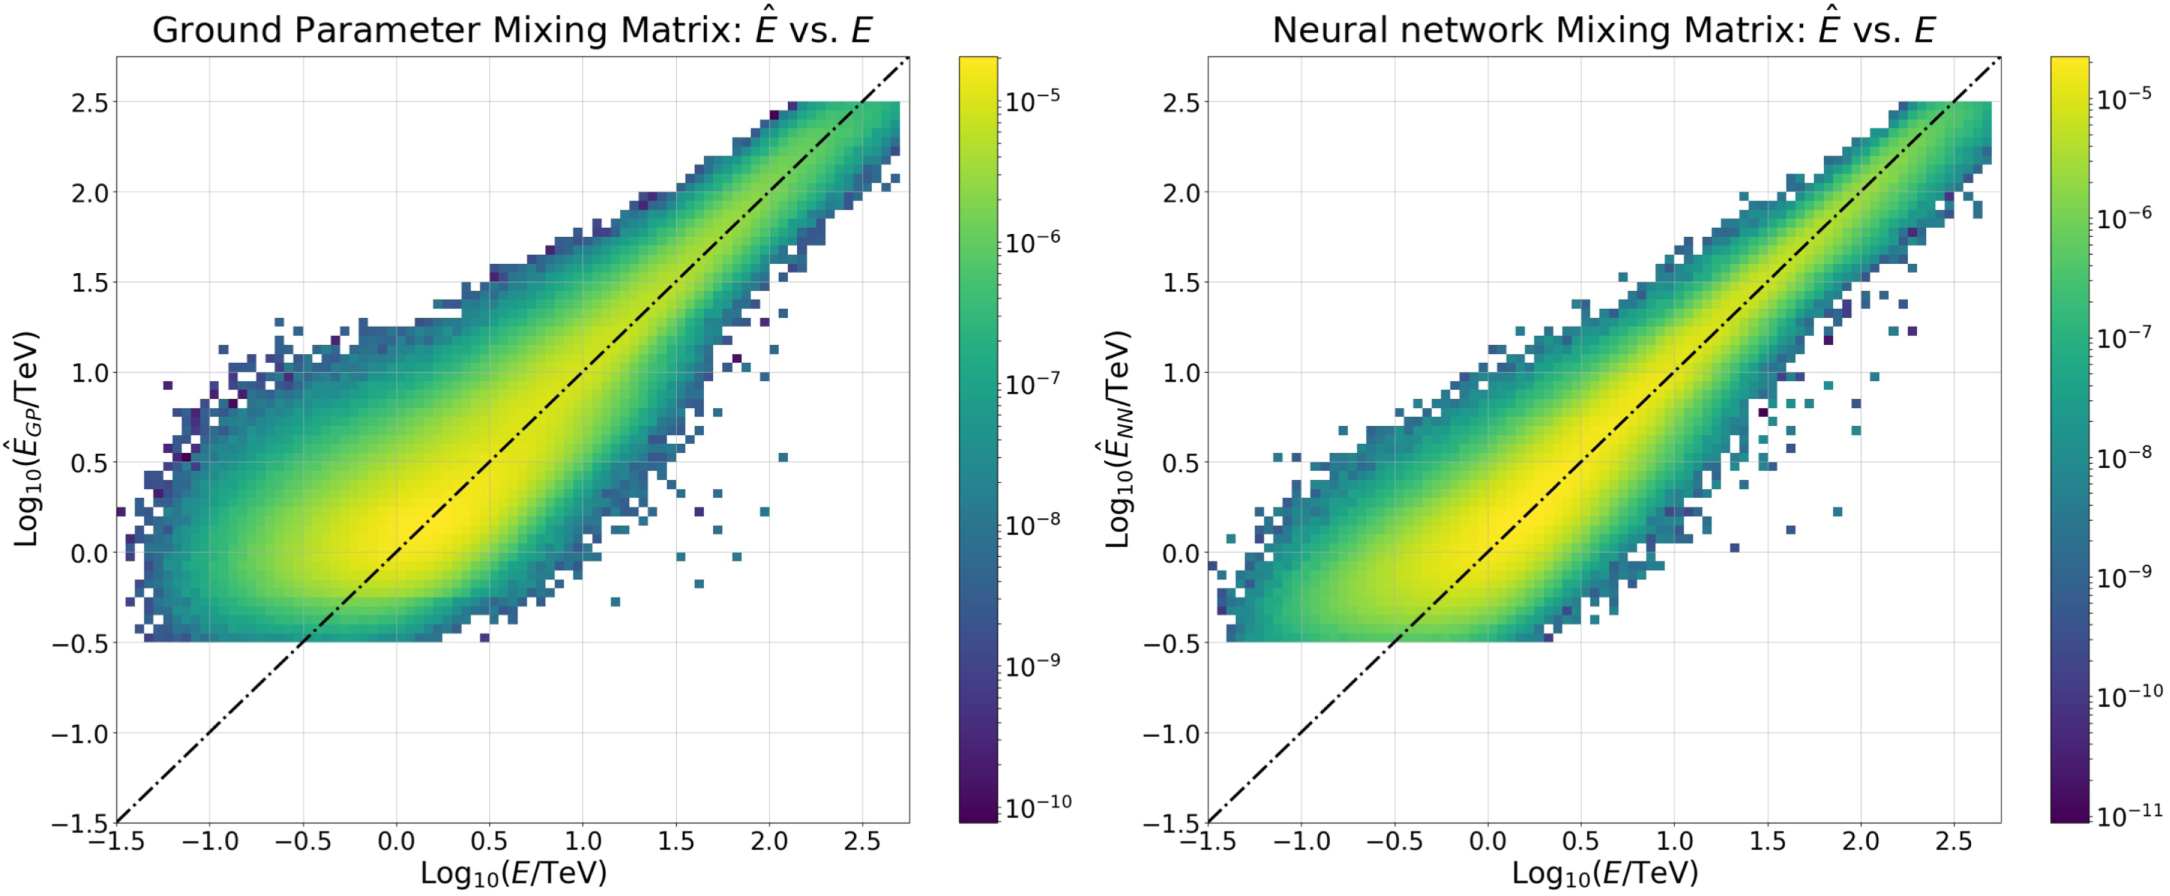
\includegraphics[clip, trim=9.1cm 0cm 0cm 0cm, scale=0.9]{figures/hawc/NN_performance.jpg}
    }
    \caption{Neural Network energy estimator performance compared to true energy. The dotted line is the identity line where the estimator and injection agree. Gamma/hadron separation cuts were applied with the energy estimation. Figure pulled from \cite{100TEV_Crab_HAWC}}
    \label{fig:NN_performance}
\end{figure}

The energy estimation for photon events at the HAWC Observatory is refined through an artificial neural network (NN) algorithm.
This method, based on the Toolkit for Multivariate Analysis NN, adopts a multilayer-perceptron model with logistic activation functions across its layers.
The structure includes two hidden layers, the first with 15 nodes and the second with 14, designed to process input variables through a neural network optimized to estimate primary particle energies \cite{thesis_SamM}.

The NN is trained to minimize a specific error function that measures discrepancies between the NN's energy predictions and the actual energies from Monte Carlo simulations.
This minimization targets an error function that incorporates the relative importance of each event, weighting more the importance to mimic an $E^{-2}$ power law spectrum.
This approach helps achieve a uniform error rate across energies ranging from 1 to 100 TeV.
The optimization process leverages the Broyden-Fletcher-Goldfarb-Shanno algorithm that calibrates the NN's 479 weights \cite{100TEV_Crab_HAWC}.

The spectral analysis employs a binned likelihood method, using a forward-folding technique to accommodate the energy estimate's bias and resolution \cite{100TEV_Crab_HAWC}.
This establishes a 2D binning scheme that categorizes events by both their $f_{\text{hit}}$ value and estimated energy.
The decision to use this scheme over a simple energy-based binning lies in the correlation between gamma/hadron separation parameters and the angular resolution with both the size and energy of the event.
The spectrum of interest is partitioned into nine $f_{\text{hit}}$ bins, each further divided into 12 energy bins, spanning from 0.316 TeV to 316 TeV, encompassing a total of 108 bins \cite{100TEV_Crab_HAWC}.
However, not all bins contribute to the final estimate.
Bins with low event populations or insufficient Monte Carlo simulation are excluded.
This approach focuses on the central 99\% of events by estimated energy within each $f_{\text{hit}}$ bin, effectively removing outliers \cite{100TEV_Crab_HAWC}.

Input variables for the NN are selected to capture key characteristics of the air shower: energy deposition, containment, and atmospheric attenuation.
The algorithm calculates energy deposition using the fraction of PMTs and tanks activated, alongside the logarithm of the normalization from the lateral distribution fit.
Containment is inferred from the distance between the shower core and the array's center, while atmospheric attenuation is evaluated using the reconstructed zenith angle and a detailed analysis of the shower's lateral charge distribution \cite{thesis_SamM,100TEV_Crab_HAWC}.

This refined NN energy estimation methodology is an integral component of HAWC's toolkit, enabling precise analysis of high-energy gamma-ray events.
It represents a significant advancement in the field by more accurately mapping observed shower characteristics to primary particle energies.

%$$$$$$$$$$$$$$$$$$$$$$$$$$$$$$$$$$$$$$$$$$$$$$$$$$$$$$$$$$$$$$$$$$$$$$$$$$$$$$$$$$$%
\subsection{G/H Discrimination}\label{hawc:gammaHadron}
%$$$$$$$$$$$$$$$$$$$$$$$$$$$$$$$$$$$$$$$$$$$$$$$$$$$$$$$$$$$$$$$$$$$$$$$$$$$$$$$$$$$%

\begin{figure}
    \centering{
        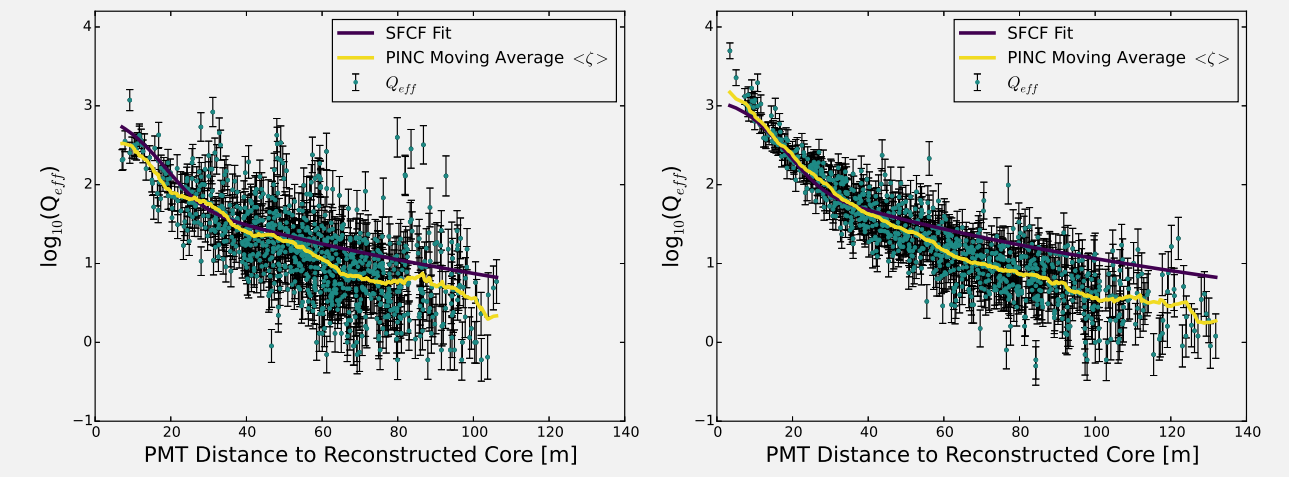
\includegraphics[scale=0.45]{figures/hawc/LDF_particles.png}
    }
    \caption{Lateral distribution functions (LDFs) for cosmic ray (left) and a photon candidate from the Crab Nebula (right). Cosmic ray LDF has clearly isolated hits far from the reconstructed shower core. Gamma-ray shower shows a more cuspy event \cite{Abeysekara_2017}.}
    \label{fig:ldf_particleshower}
\end{figure}

At the HAWC Observatory, distinguishing between air showers initiated by gamma rays and those by hadronic cosmic rays is fundamental for astrophysical data purity.
The separation process leverages differences in shower characteristics: electromagnetic showers from gamma rays typically display fewer muons and a smoother lateral distribution, whereas hadronic showers are more chaotic due to the abundance of muons and hadronic sub-showers.

Two primary parameters facilitate the identification of cosmic-ray events \cite{Abeysekara_2017}:

Compactness (C): This parameter evaluates the charge captured by PMTs, particularly focusing on the PMT with the highest effective charge beyond a 40-meter radius from the shower core.
Compactness is inversely proportional to this effective charge, as higher charges at extended distances from the core are indicative of hadronic showers.
It is mathematically expressed as:
\compactness
where $N_\mathrm{hit}$ is the number of PMTs hit and $CxPE_{40}$ is the effective charge measured outside a 40 m radius from the shower cores \cite{Abeysekara_2017}.

PINCness (P): PINCness quantifies the "clumpiness" of a shower using the charges recorded by PMTs and is short for Parameter for Identifying Nuclear Cosmic Rays.
It is computed from the logarithm of the effective charge, $Q_{\mathrm{eff},i}$, of each PMT hit, $i$, compared to an expected average for that annular region.
A higher PINCness suggests a less smooth distribution, typical of hadronic showers.
The formula is:
\pincness
where $\zeta_i = \log_{10}(Q_{\mathrm{eff},i})$.
The average, $\langle \zeta \rangle$ is the average over an anular region surrounding the shower core.
The errors, $\sigma_{\zeta_i}$, are computed and allocated from gamma-ray candidates close to the Crab.

These parameters are tested and modeled in simulations and with observational data near the Crab Nebula.
\Cref{fig:ldf_particleshower} illustrating the lateral distributions for representative cosmic-ray and photon candidate showers, as well as the distribution of these discrimination parameters, affirm their efficacy \cite{Abeysekara_2017}.

The discrimination technique has remained consistent, but cut values have been reoptimized for the 2D bins based on $f_{\text{hit}}$ and NN estimated energy.
This refinement enhances the selection of high-energy events.
Each bin ensures at least 50\% efficiency for gamma-ray detection, with efficiencies extending up to nearly 100\% in certain bins \cite{Abeysekara_2017,100TEV_Crab_HAWC}.

%$$$$$$$$$$$$$$$$$$$$$$$$$$$$$$$$$$$$$$$$$$$$$$$$$$$$$$$$$$$$$$$$$$$$$$$$$$$$$$$$$$$%
\section{Background Estimation: Direct Integration}\label{hawc:direc_int}
%$$$$$$$$$$$$$$$$$$$$$$$$$$$$$$$$$$$$$$$$$$$$$$$$$$$$$$$$$$$$$$$$$$$$$$$$$$$$$$$$$$$%

The ratio of cosmic rays to gamma rays can be as high as 10,000 to 1, depending on the energy.
At HAWC, we confront a significant challenge even after gamma/hadron cuts: our gamma-ray data is still inundated with cosmic-ray events.
To tackle this, we rely on the direct integration method developed by Milagro \cite{Milagro_crab}.
This method capitalizes on the cosmic rays' isotropic nature resulting from their deflection by interstellar magnetic fields.

The direct integration method estimates background events by integrating over a stable two-hour period of detector operation.
The expected number of background events at a particular sky coordinate ($\phi, \theta$) is determined by integrating the normalized detector's efficiency with the all-sky event rate:
\directInt
Here, $E(\text{ha}, \theta)$, represents the detector's efficiency, which varies with local coordinates (hour angle and declination).
$R(t)$ is the event rate as a function of time \cite{Milagro_crab}.

Our background estimation is expected to falter in high-energy ranges where cosmic-ray events are less frequent due to enhanced gamma/hadron discrimination. Sparsity in our background and data also arise at the limits of HAWC's sensitivity and during short-term analyses of transient events.
HAWC addresses these issues by using a pixel size of 0.5$^\circ$ in our direct integration to maintain robustness in our estimation \cite{Abeysekara_2017,wcd_Sensitivity}.
In constructing the background model, it's crucial to exclude areas of the sky with known gamma-ray sources.
Regions containing the Crab Nebula, Mrk 421, Mrk 501, and the Galactic Plane are masked to prevent their significant gamma-ray signals from biasing our background estimate \cite{Abeysekara_2017}.


%%%%%%%%%%%%%%%%%%%%%%%%%%%%%%%%%%%%%%%%%%%%%%%%%%%%%%%%%%%%%%%%%%%%%%%%%%%%%%%%%%%%%
\chapter{IceCube Neutrino Observatory\label{sec:ice3}}
%%%%%%%%%%%%%%%%%%%%%%%%%%%%%%%%%%%%%%%%%%%%%%%%%%%%%%%%%%%%%%%%%%%%%%%%%%%%%%%%%%%%%
\begin{figure}[h!]
    \centering{
        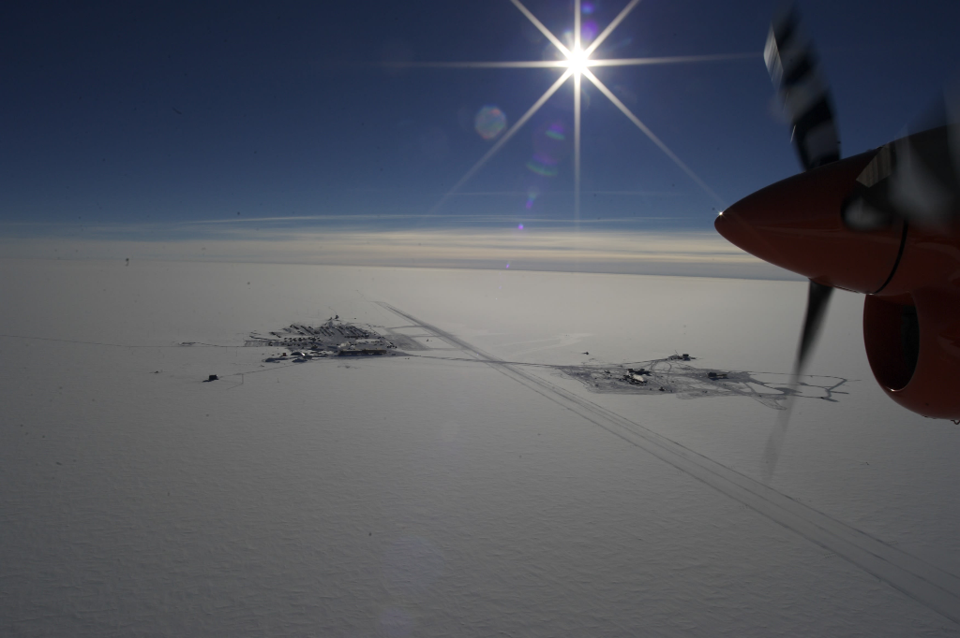
\includegraphics[clip, trim=3cm 3.5cm 2cm 0cm, scale=0.8]{figures/ic3/IC3_aboveground.png}
    }
    \caption{IceCube Neutrino observatory and science center at the South Pole. Detector volume is beneath glacial ice. Image from \cite{IceCube_SPGallery}.}
    \label{fig:IC3_atPole}
\end{figure}

Located at the South Pole, the IceCube Neutrino Observatory is a pivotal instrument for neutrino astronomy.
The above and below ice components of the IceCube observatory are shown in \cref{fig:IC3_atPole,fig:IC3_full_detector}.
IceCube's primary function is the detection and analysis of elusive, high-energy neutrinos.
These neutrinos carry information from the most energetic and distant cosmic phenomena.
The observatory uses thousands of digital optical modules embedded in a cubic kilometer of Antarctic ice to detect Cherenkov radiation.
This radiation occurs when neutrinos interact with the ice, revealing their origin and energy.

IceCube is a critical component in the multi-messenger astrophysics toolkit, especially in the search for dark matter and beyond standard model (BSM) astrophysical processes.
The observatory's analysis of neutrino signals enhances our understanding of the universe by correlating these signals with other cosmic messengers, including electromagnetic, gravitational waves, and cosmic rays.
The following sections will discuss the observatory's design, data acquisition, and event reconstruction methodologies.

%-----------------------------------------------------------------------------------%
\section{The Detector}
%-----------------------------------------------------------------------------------%

\begin{figure}
    \centering{
        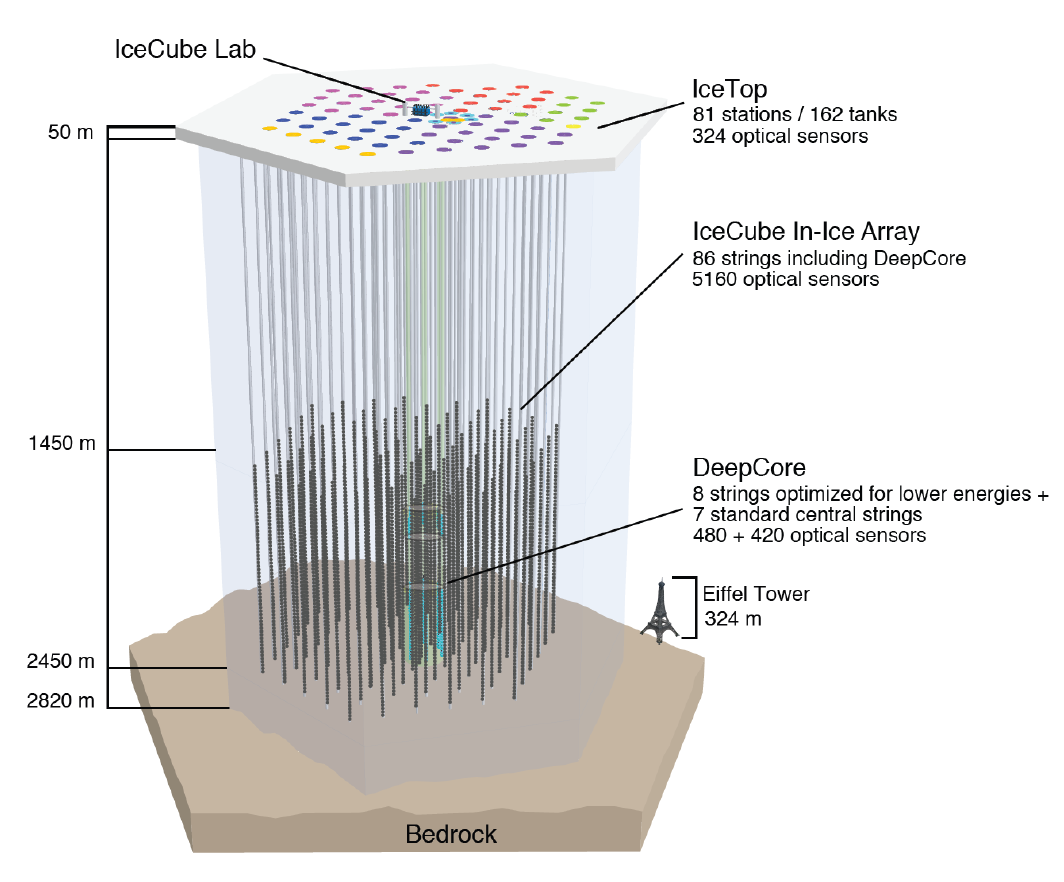
\includegraphics[scale=0.5]{figures/ic3/icecube.png}
    }
    \caption{Graphic of the full IceCube Neutrino Observatory. In-ice array is made up of 86 strings with a total of 5160 optical sensors. Deepcore is a denser arrangement of optical sensors for sensitivity to lower energy neutrinos. Figure from \cite{IceCube_SPGallery}.}
    \label{fig:IC3_full_detector}
\end{figure}

The IceCube Neutrino Observatory is embedded within a cubic kilometer of Antarctic ice at the South Pole.
IceCube's modules are designed to detect neutrinos through Cherenkov radiation emitted after neutrino interactions within the ice.
It comprises of 5160 Digital Optical Modules (DOMs), arranged across 86 strings that span depths of 1450 m to 2450 m beneath the surface.
This arrangement allows IceCube to capture high-energy neutrinos across a broad neutrino energy spectrum.

%$$$$$$$$$$$$$$$$$$$$$$$$$$$$$$$$$$$$$$$$$$$$$$$$$$$$$$$$$$$$$$$$$$$$$$$$$$$$$$$$$$$%
\subsection{Hardware and Construction}
%$$$$$$$$$$$$$$$$$$$$$$$$$$$$$$$$$$$$$$$$$$$$$$$$$$$$$$$$$$$$$$$$$$$$$$$$$$$$$$$$$$$%

\begin{figure}
    \centering{
        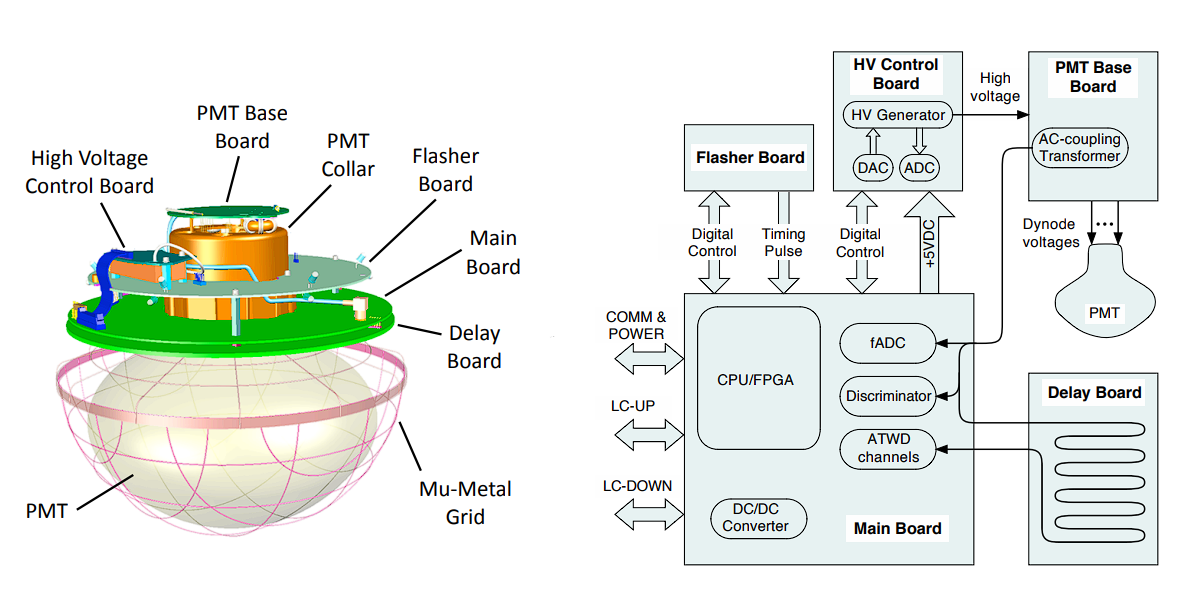
\includegraphics[scale=0.5]{figures/ic3/DOM.png}
    }
    \caption{Composition of the Digital Optical Module (DOM). Left image is an illustration of the mechanical layout. Right is a flow chart of functional connections. Figure from \cite{IC3_thedetector}}
    \label{fig:DOM}
\end{figure}

Digital Optical Modules (DOMs) are at the core of IceCube’s detection technology.
\Cref{fig:DOM} illustrates the construction and signal flow of a DOM.
Each DOM is encased in a glass sphere that can withstand deep-ice pressures.
A DOM features a 10-inch PMT for Cherenkov light detection, a high-voltage power supply for the PMT, and a Main Board for signal digitization and timestamping.
An LED Flasher Board is included for calibration purposes.
They assist in verifying DOM responses and measuring the glacial ice's optical properties.
The DOMs are deployed along cables on strings in a hexagonal grid pattern that spans a cubic kilometer.
Strings are placed with 125 m of horizontal spacing, and DOMs are vertically separated by 17 m on each string.
This detector geometry optimizes detection of TeV to PeV neutrinos.

DeepCore and IceTop, additional components of IceCube, extend its research capabilities.
DeepCore, with its denser array of DOMs, targets lower energy neutrinos for studies such as neutrino oscillations.
IceTop, situated at the ice surface, measures cosmic rays, contributing data that complement the neutrino observations from below the ice.
\Cref{fig:IC3_full_detector} illustrates the full detector volume and auxiliary systems.

The central hub for IceCube's operations is the IceCube Laboratory (ICL) and is situated at the surface at the center of the array (see \cref{fig:ICL}).
This facility houses the servers and computers responsible for data acquisition and online filtering.
ICL connects to the DOMs via cables routed up from beneath the ice \cite{IC3_thedetector}.
The ICL manages the data flow from the ice, ensuring continuous operation and data integrity.
It maintains optimal conditions for its electronic equipment, including temperature control and protection against electromagnetic interference \cite{IC3_thedetector}.


%$$$$$$$$$$$$$$$$$$$$$$$$$$$$$$$$$$$$$$$$$$$$$$$$$$$$$$$$$$$$$$$$$$$$$$$$$$$$$$$$$$$%
\subsection{Data Acquisition}
%$$$$$$$$$$$$$$$$$$$$$$$$$$$$$$$$$$$$$$$$$$$$$$$$$$$$$$$$$$$$$$$$$$$$$$$$$$$$$$$$$$$%

\begin{figure}
    \centering{
        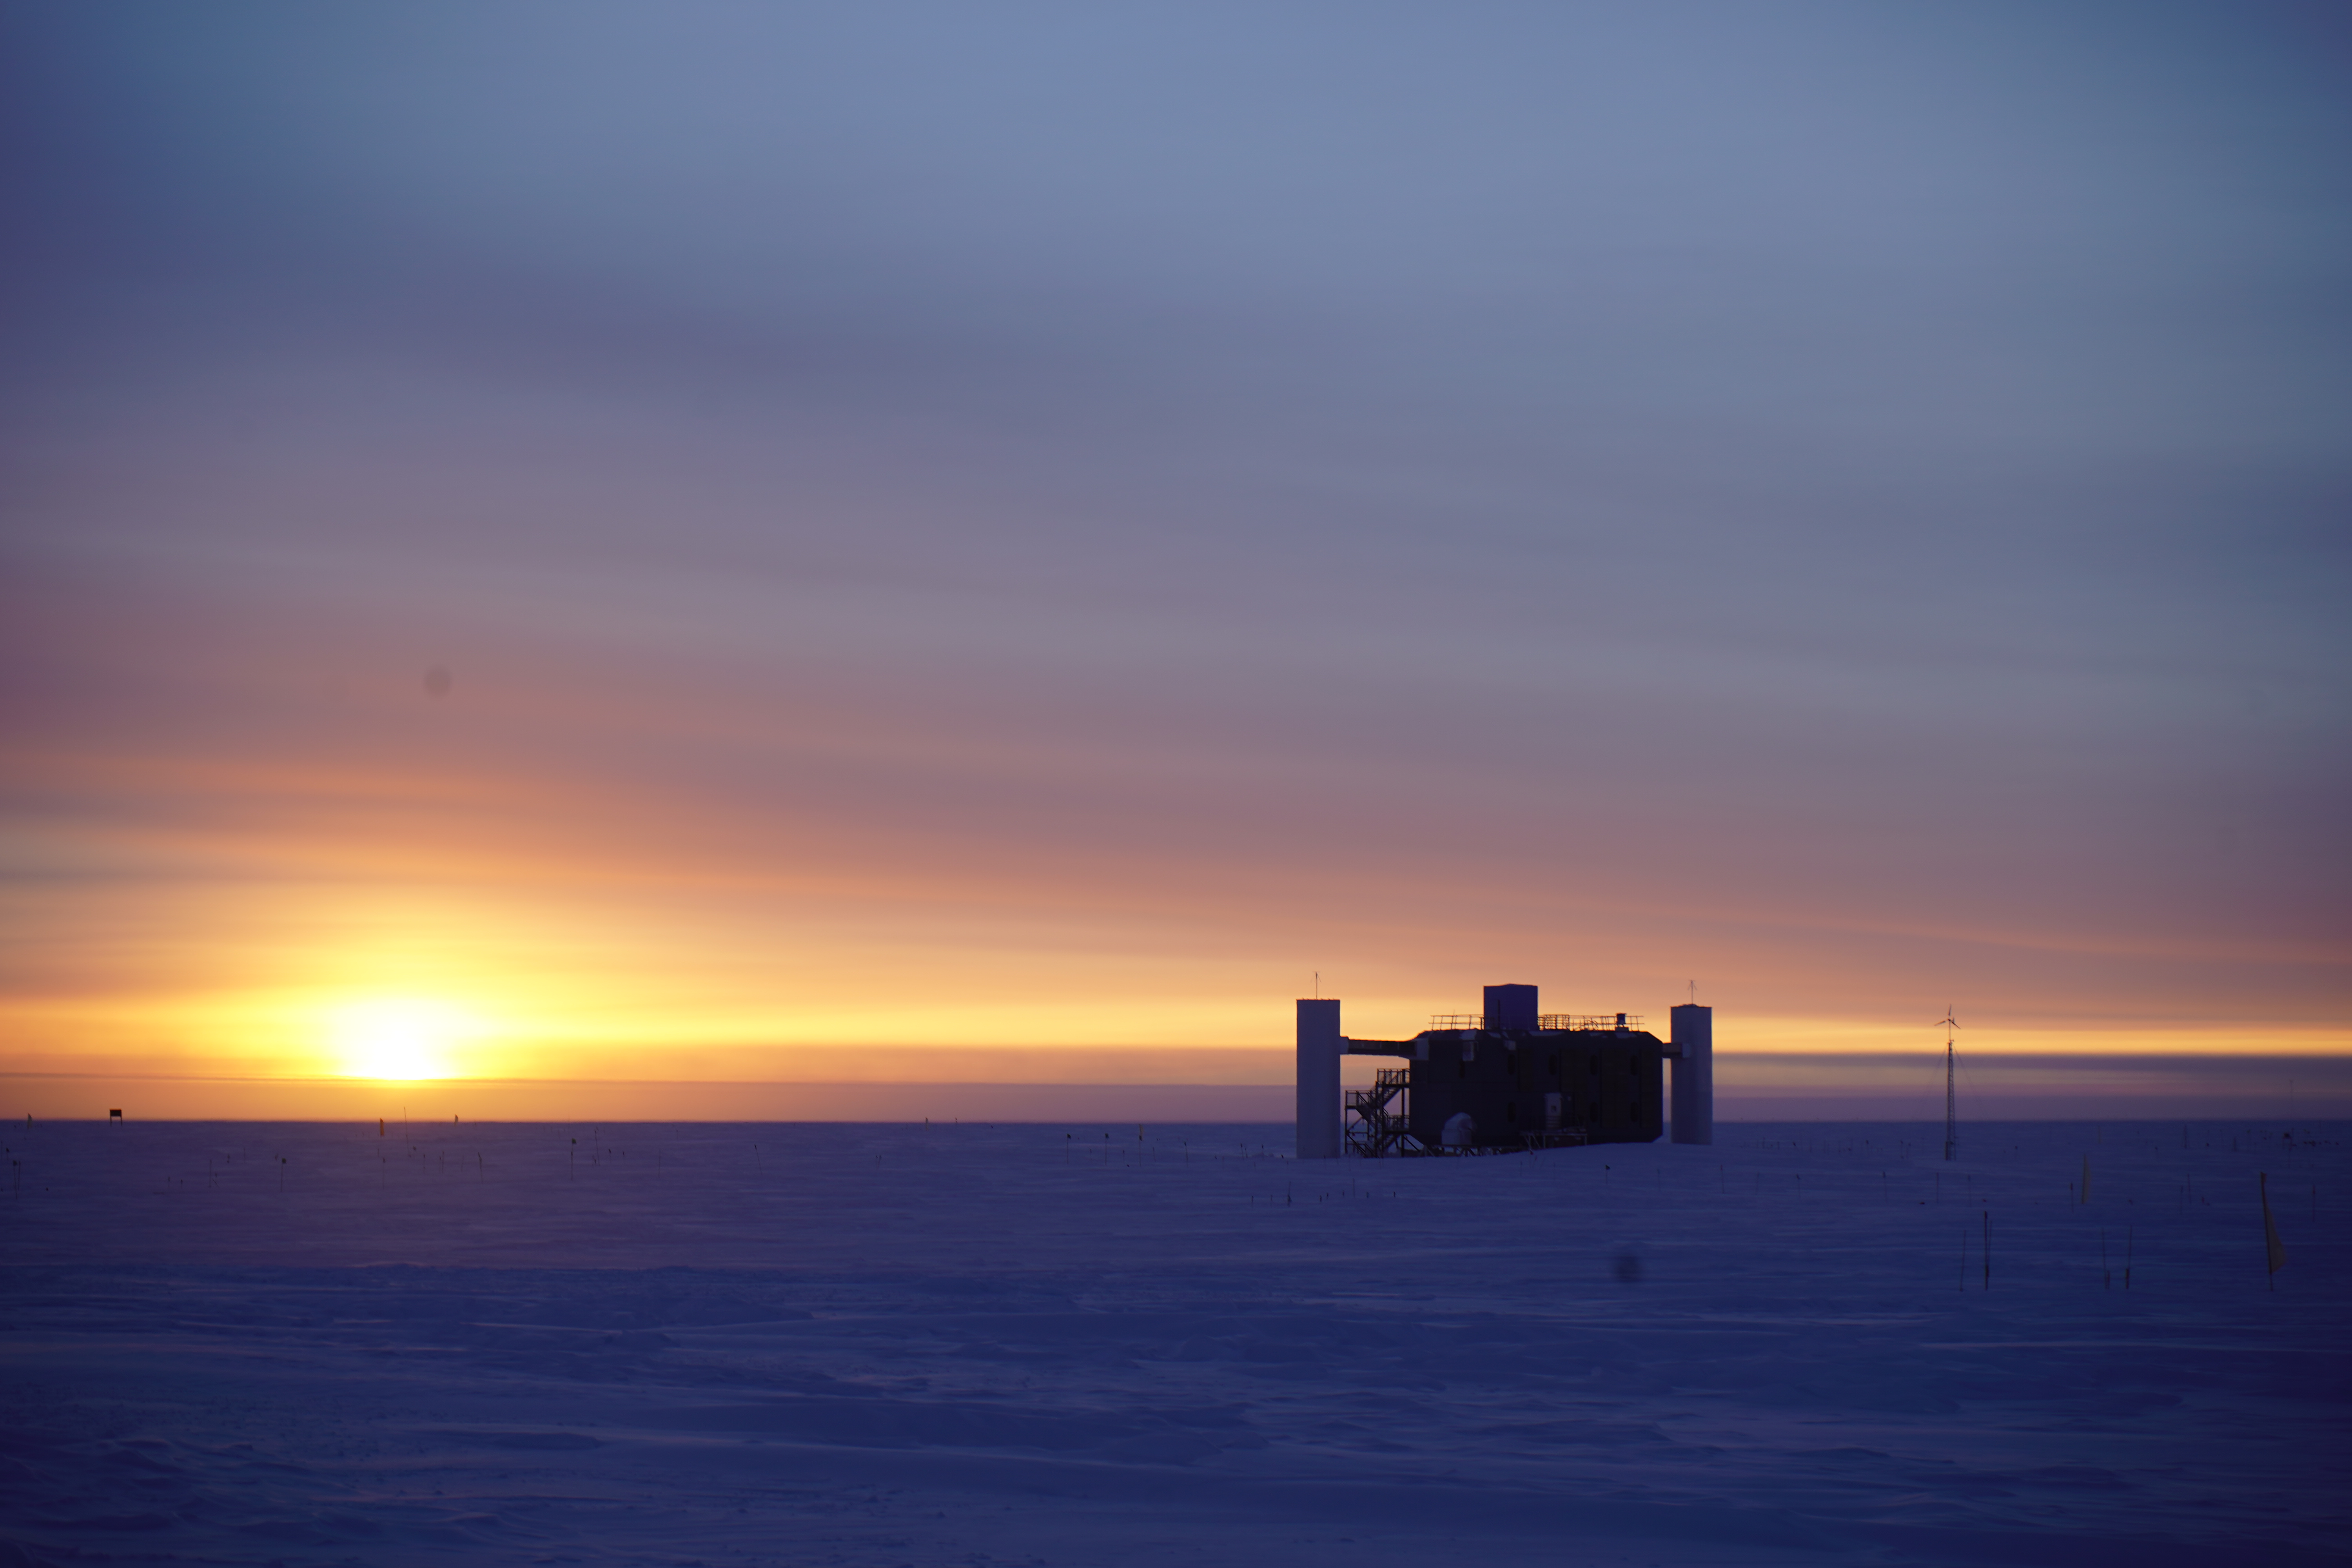
\includegraphics[scale=0.37]{figures/ic3/ICL.JPG}
    }\caption{IceCube Laboratory (ICL) that houses the data acquisition systems. Picture from \cite{IceCube_SPGallery}.}
    \label{fig:ICL}
\end{figure}

\begin{figure}
    \centering{
        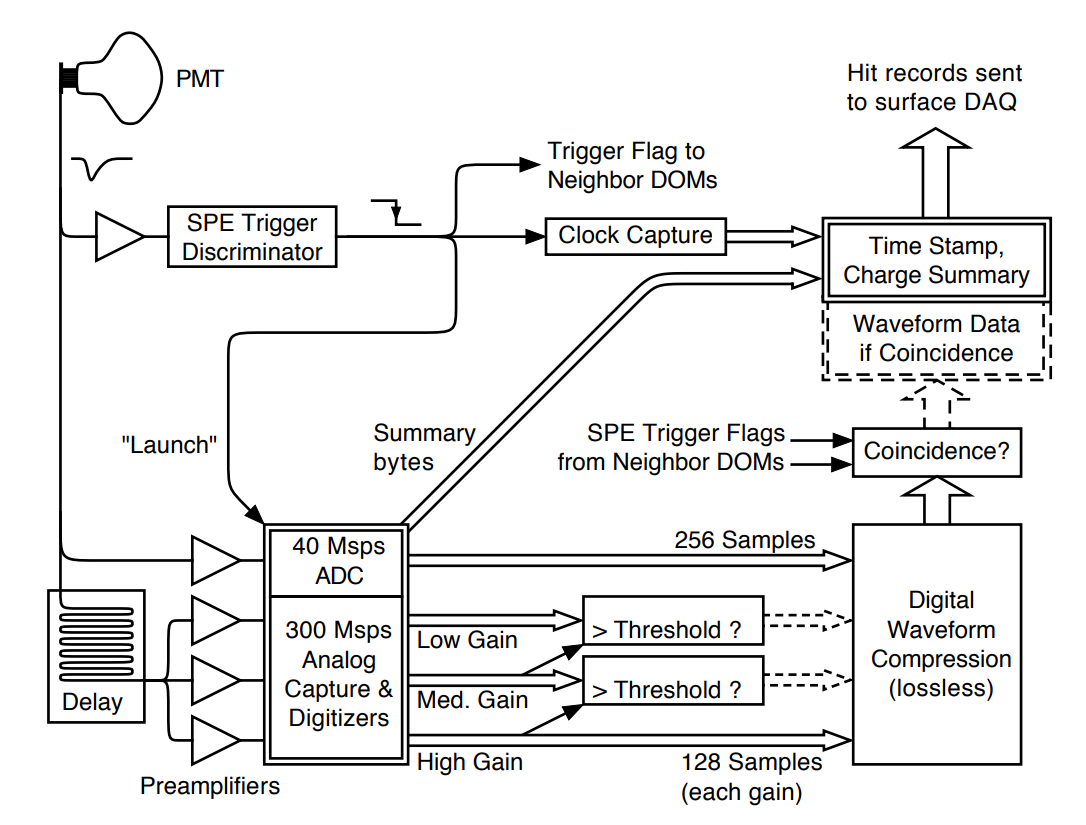
\includegraphics[scale=0.4]{figures/ic3/IC3_dataflow.png}
    }
    \caption{Data flow chart PMT waveforms from the DOMs. “Hit Records" are sent to the surface DAQ computers in ICL. Full waveform data, represented with dashed arrows, are included when neighboring DOMs are hit in coincidence above the SPE discriminator threshold.}
    \label{fig:IC3_dataflow}
\end{figure}

The data acquisition process in IceCube starts when a PMT within a DOM detects light surpassing a threshold of 0.25 photoelectrons.
The importance of the information transmitted to the ICL depends on the detection of hits in neighboring DOMs within a microsecond window.
Isolated signals prompt a Soft Local Coincidence (SLC) response, transmitting only a timestamp and a charge summary.
In contrast, signals detected by neighboring DOMs initiate a Hard Local Coincidence (HLC).
The full waveform is compressed and sent along with the timestamp and charge summary to the ICL \cite{IC3_thedetector}.
\Cref{fig:IC3_dataflow} shows a flow chart of PMT data within the DOMs before being sent to the ICL.

Achieving uniform timing across DOMs is essential for accurate event reconstruction.
Each DOM's independent clock is finely calibrated and synchronized with the ICL's clocks.
Times are translated to Universal Coordinated Time (UTC).
This calibration is set by sending continuous pulses between the DOMs and the ICL.
The waveforms are adjusted by subtracting the common baseline and applying the gain \cite{IC3_thedetector}.

Within the ICL, the Data Acquisition (DAQ) system employs various trigger algorithms to discern neutrino events from the vast majority of DOM hits caused by dark noise.
One such mechanism, the Simple Multiplicity Trigger (SMT), requires a specific number of HLC hits within a brief timeframe to recognize a series of hits as an event \cite{IC3_thedetector}.

Further refining the observatory's data, the Processing and Filtering (PnF) system, also housed within the ICL, applies around 25 different filters after initial event detection.
Each filter is designed for specific physics analyses.
The system employs filters such as: The Muon Track Filter to isolate high-quality track events crucial for neutrino source identification;
the Shower Event Filter to select events with large energy deposits indicative of neutrino interactions;
and the High-Charge Filter to highlight events with extensive photoelectron deposits \cite{IC3_thedetector}.
These filters ensure that the data prepared for further analysis and transmission to researchers in the Northern Hemisphere contains the most significant scientific insights \cite{IC3_thedetector}.

The operational control of the observatory, maintained by the LiveControl system within the ICL, oversees the DAQ and PnF systems.
It handles the initiation and conclusion of data-taking runs and maintains a database of operational parameters.
LiveControl alerts operators to any deviations from expected conditions.
It is crucial for ensuring that the observatory operates within its optimal parameters \cite{IC3_thedetector}.

%-----------------------------------------------------------------------------------%
\section{Event Reconstruction}
%-----------------------------------------------------------------------------------%
Event Reconstruction within the IceCube Neutrino Observatory transforms signals captured by DOMs into quantifiable scientific insights.
The goal of event reconstruction is to ascertain the origin, trajectory, and energy of interacting neutrinos.
This process is pivotal for interpreting signals as either originating from celestial neutrino sources or other phenomena.
I will focus mostly on how IceCube reconstructs track-like events as these are the most relevant for this dissertation.

%$$$$$$$$$$$$$$$$$$$$$$$$$$$$$$$$$$$$$$$$$$$$$$$$$$$$$$$$$$$$$$$$$$$$$$$$$$$$$$$$$$$%
\subsection{Tracks and Cascades}
%$$$$$$$$$$$$$$$$$$$$$$$$$$$$$$$$$$$$$$$$$$$$$$$$$$$$$$$$$$$$$$$$$$$$$$$$$$$$$$$$$$$%

\begin{figure}
    \centering{
        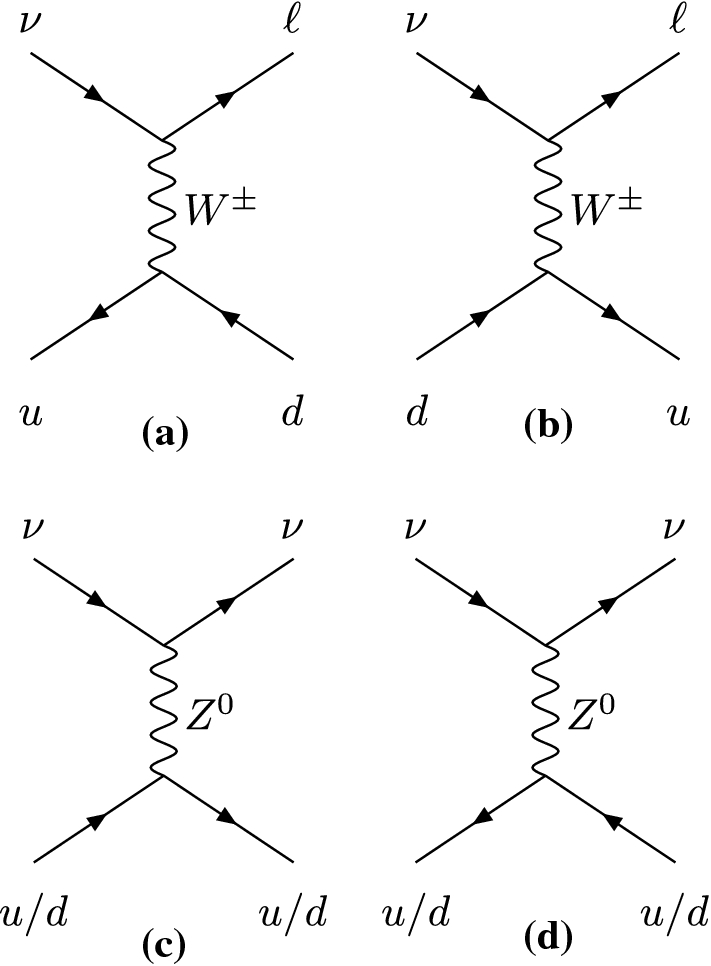
\includegraphics[scale=0.3]{figures/ic3/nn_cc_feynman.png}
    }
    \caption{Feynman diagrams for W (a/b) and Z (c/d) boson mediated interactions between neutrinos and light quarks. Charged current (CC) interactions are shown in panels a and b. Neutral current (NC) interactions are shown in panels c and d. NC interactions occur between neutrinos and quarks within atomic nucluei in the ice. CC interactions will exchange W bosons and produce a lepton corresponding to the neutrino flavor and a hadronic cascade. NC interactions will exchange a Z boson and produce a hadronic cascades. Figure from \cite{physics_withIC3}.}
    \label{fig:ic2_ccORnc}
\end{figure}

\begin{figure}
    \centering{
        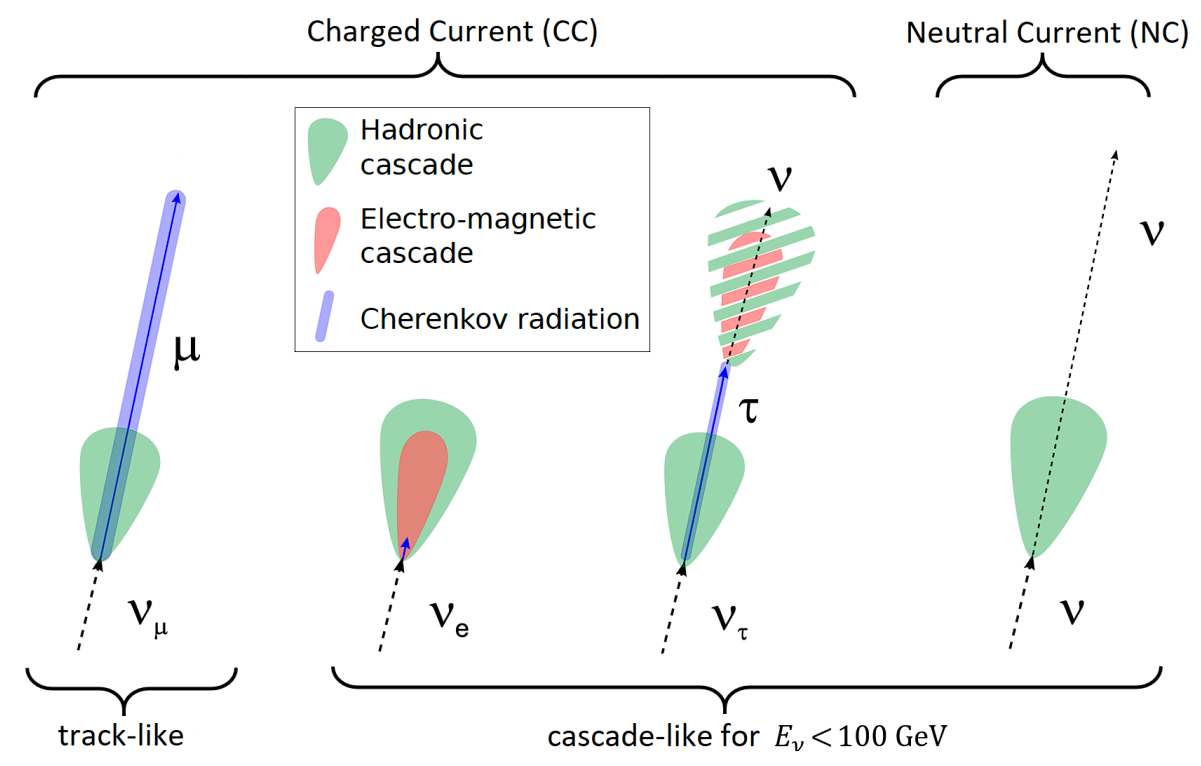
\includegraphics[scale=0.4]{figures/ic3/event_topologies.png}
    }
    \caption{Event topologies for high energy NC and CC neutrino interactions with ice. Signatures can be split as either: hadronic and electromagnetic cascades; Cherenkov radiation from a charged, long-lived particle. Cascades from $\tau$ decays will depend on its decay products. For energies below 1 PeV the double bang of the $\nu_\tau$ signature overlap and are indistinguishable. Figure from \cite{rene_thesis_nutracks}.}
    \label{fig:event_topology}
\end{figure}

\begin{figure}
    \centering{
        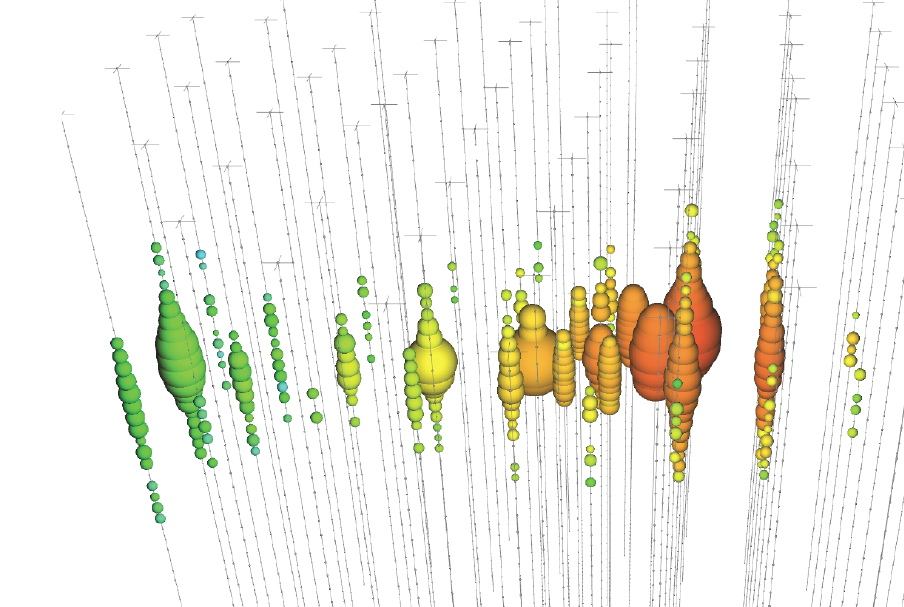
\includegraphics[scale=0.5]{figures/ic3/neutrinos-track-sig-2.png}
    }
    \caption{A simulation of a track-like event in IceCube. Redder bubbles indicate earlier photon arrival times. Greener bubbles occur later. The size of the DOM bubble illustrate the charge deposition in the DOM. For this event, the CC neutrino interaction occurred by the red hits. There is then a long muon track going to the left. Figure taken from \cite{IC3_masterclass}.}
    \label{fig:ic3_track}
\end{figure}

\begin{figure}
    \centering{
        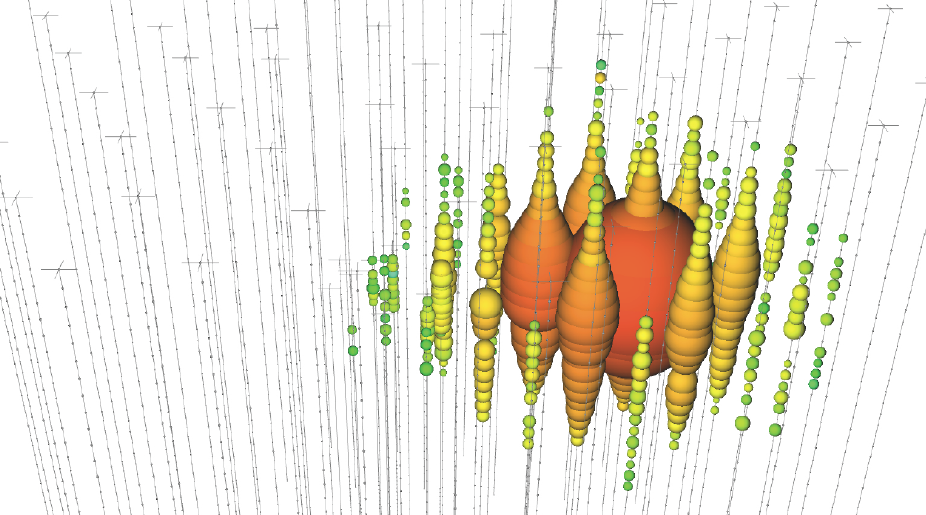
\includegraphics[scale=0.5]{figures/ic3/neutrinos-cascade-sig-1.png}
    }
    \caption{Same as \cref{fig:ic3_track} but for a cascade-like event. Figure taken from \cite{IC3_masterclass}.}
    \label{fig:ic3_cascade}
\end{figure}

\begin{figure}
    \centering{
        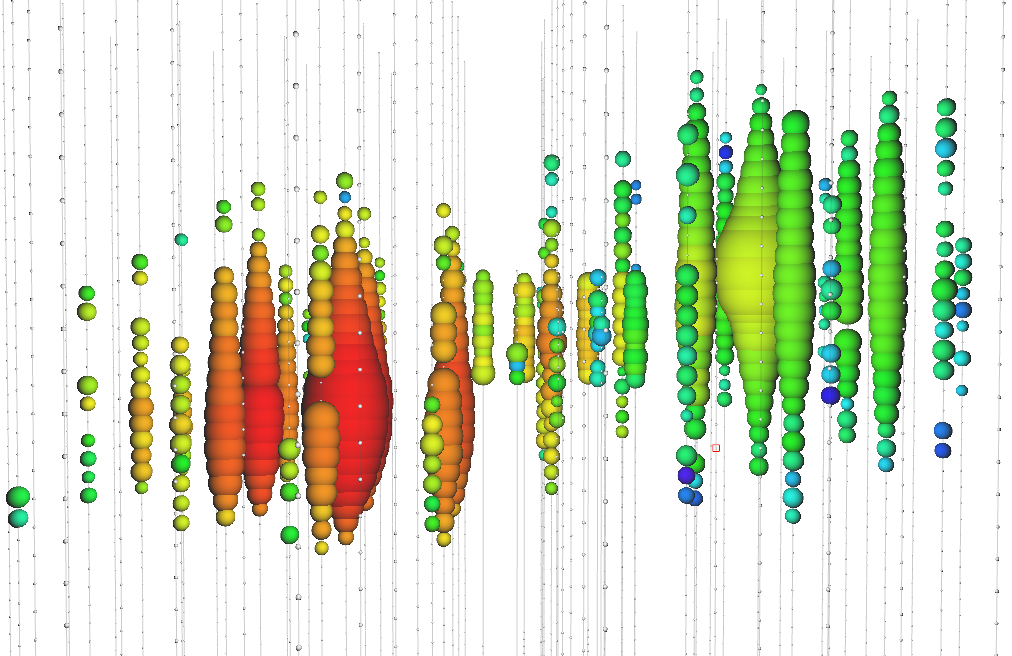
\includegraphics[scale=0.45]{figures/ic3/neutrinos-double-bang-sig-3.png}
    }
    \caption{Same as \cref{fig:ic3_track} but for a double-bang event. Two distinct cascades are visible if the initial neutrino is very high energy. Figure taken from \cite{IC3_masterclass}.}
    \label{fig:ic3_doubleBang}
\end{figure}

Events in IceCube's detector volume manifest primarily as either tracks or cascades.
The primary cause of the event topology are both the neutrino flavor and the nature of the primary neutrino's interaction with the ice.
\Cref{fig:ic2_ccORnc} presents Feynman diagrams of typical neutrino interactions with particles in the ice.
\Cref{fig:event_topology} illustrates the signatures from various topologies of neutrino interactions in the ice.

Tracks emerge from charged-current (CC) interactions involving muon neutrinos ($\nu_\mu$).
These events are characterized by the production of a high-energy muon ($\mu$).
These muons, due to its relatively large mass compared to electrons, can traverse substantial distances through the ice, exceeding kilometers.
These long trajectories are obvious from their continuous, distinct, and elongated track of Cherenkov light in the ice.
See \cref{fig:ic3_track} for a simulated track event.
The angular deviation between the incoming $\nu_\mu$ and the secondary $\mu$ is notably slight, tapering to near 0.3$^\circ$ above TeV energies.
Therefore, $\mu$ tracks closely approximate the primary neutrino's path \cite{physics_withIC3,IC3_energyReco}.
Such precision affords angular resolutions finer than 1$^\circ$ for TeV neutrinos which facilitates the determination of their cosmic origins \cite{physics_withIC3}.

Cascades are products of both neutral-current (NC) interactions across all neutrino flavors and CC interactions involving electron or tau neutrinos, $\nu_e$ and $\nu_\tau$ respectively.
Unlike tracks, cascades result in a more localized burst of Cherenkov radiation.
The burst imprints as a nearly spherical light pattern from the rapid dissipation of energy by the produced particles.
See \cref{fig:ic3_cascade} for a simulated track event.
This diffusion creates a distinct event signature with good energy estimation, but worse directional clarity compared to track events.
The isotropic nature of cascades leads to larger angular uncertainties, typically around 15$^\circ$.
Yet, cascades excel in providing energy measurements, with resolutions reaching as tight as 15\% from the contained nature of the energy deposition \cite{physics_withIC3,IC3_energyReco}.

The double-bang event, posited for $\nu_\tau$ interacting via CC at energies above 1 PeV, would display as two distinct cascades within the detector.
These events start from an initial interaction and subsequent decay of the $\tau$ lepton over a discernible distance.
See \cref{fig:ic3_doubleBang} for a simulated track event.
The double-bang offers a unique marker for high-energy $\nu_\tau$ detection \cite{physics_withIC3}.
Preliminary whispers of double-bang events IceCube have been observed \cite{IC3_taus}.
Yet, efforts are ongoing to isolate such an event.

%$$$$$$$$$$$$$$$$$$$$$$$$$$$$$$$$$$$$$$$$$$$$$$$$$$$$$$$$$$$$$$$$$$$$$$$$$$$$$$$$$$$%
\subsection{Reconstruction of Track Direction}
%$$$$$$$$$$$$$$$$$$$$$$$$$$$$$$$$$$$$$$$$$$$$$$$$$$$$$$$$$$$$$$$$$$$$$$$$$$$$$$$$$$$%

Angular reconstruction for $\nu_\mu$ induced tracks in the IceCube detector volume starts with the LineFit algorithm \cite{AMANDA_trackreco}.
LineFit estimates the $\mu$'s trajectory through the least squares fit to the Cherenkov light hits on the DOMs.
LineFit assumes the muon propagates with constant velocity and treats its path as linear in order to simplify the emission patterns of Cherenkov radiation.
To improve this approximation, the Huber penalty function \cite{Huber:1964} is applied which distinguishes between signal and noise by considering the spatial distribution of hits relative to the track \cite{IC3_Calibration}.

The reconstruction process is refined further by the Single Photoelectron (SPE) likelihood method, which calculates the probability of photon arrival times at the DOMs \cite{Huber:1964}.
It does so by taking into account the earliest detected photons as they are least likely to have been scattered in the ice:
\spe
where $N_{\mathrm{DOM}}$ is the number of DOMs involved in the event.
$N_{\mathrm{hit}}$ is the number of hits registered \cite{AMANDA_trackreco}.
$p_j(t_i)$ is the probability density function (PDF) of the photon arrival time.
The charge detected by each DOM, $q_i$, factors into the probability calculation, assuming that earlier photons provide more reliable directional information.

An alternative to SPE, the Multi-Photoelectron (MPE) likelihood method accounts for all detected photons.
MPE uses the total observed charge to weight the significance of each hit:
\mpe
where $Q_j$ is the sum of charges observed by the j-th DOM, providing a more detailed picture of the $\mu$'s path \cite{AMANDA_trackreco}.

SplineMPE, is the final step and employs a spline-based parameterization of the photon arrival times.
These spline fits encode a detailed understanding of the ice's optical properties derived from calibration data \cite{AMANDA_trackreco}.
This approach yields the following likelihood function for improved angular resolution:
\splineMPE
where the parameters $\vec{r_0}, t_0, \theta, \mathrm{ and}~\phi$ describe the reconstructed track within IceCube's voluminous array \cite{AMANDA_trackreco}.

From the light weight LineFit to the complex SplineMPE, each step incorporates more detailed physics to enhance the reconstruction's accuracy.
Each hones in on the $\mu$ track to reveal the $\mu$'s cosmic origin.
This multi-stepped tracking is crucial for IceCube's mission to map the universe through the lens of high-energy neutrino interactions.

%$$$$$$$$$$$$$$$$$$$$$$$$$$$$$$$$$$$$$$$$$$$$$$$$$$$$$$$$$$$$$$$$$$$$$$$$$$$$$$$$$$$%
\subsection{Energy}
%$$$$$$$$$$$$$$$$$$$$$$$$$$$$$$$$$$$$$$$$$$$$$$$$$$$$$$$$$$$$$$$$$$$$$$$$$$$$$$$$$$$%

After pinpointing the $\mu$ track's direction, IceCube employs the MuEX algorithm to estimate the energy deposited by the muon inside the detector.
The MuEX algorithm uses a Poisson likelihood model, comparing the observed photoelectrons $k$ to the expected light output, $\Lambda$, which is directly related to the deposited energy $E$:
\muEXLLH
$\rho$ is the number of expected noise photons, and $\Lambda$ reflects the light yield per unit energy, taking into account the optical properties of the ice and the detector response.
The logarithm of the likelihood is minimized with respect to the energy, resulting in a best-fit estimate \cite{IC3_energyReco}.

For a more detailed energy reconstruction, the Millipede algorithm unfolds the muon's energy loss along its path by adapting the Poisson likelihood.
This approach accounts for the stochastic energy losses due to Bremsstrahlung and pair production, treating the $\mu$ as a series of electromagnetic cascades:
\vecMULLH
where $k$ denotes the observed photons, $\rho$ the noise, $E$ the energy losses, and \textbf{$\Lambda$} the matrix of predicted light yields throughout the detector.
By fitting the muon's position, direction, and the vector of energy losses, Millipede achieves a resolution on total deposited energy along the muon track of approximately 10-15\% \cite{IC3_energyReco}.

IceCube makes some approximations when estimating $\lambda$ for the reduction of computational time.
Two important assumptions IceCube makes are that Cherenkov light from cascades is spherically symmetric along the $\mu$ track and the Cherenkov emission is uniform \cite{IC3_energyReco}.
The uncertainties in these approximations is accounted for by convolving $\lambda$ with a PDF, $G$, on the light yield.
The likelihood is then rewritten as:
\LLHwithspice
The full description for the PDF, $G(\lambda_i, \lambda_j)$ is discussed in \cite{IC3_energyReco}.
After considering the uncertainties, the energy resolution was observed to be in the range of 30\%-35\% \cite{IC3_energyReco}.

%-----------------------------------------------------------------------------------%
\section{Background}
%-----------------------------------------------------------------------------------%

In IceCube, the primary challenge in detecting astrophysical neutrinos is the background noise from atmospheric neutrinos.
These are produced from cosmic rays hitting the Earth's atmosphere, leading to a cascade that includes both neutrinos and muons (see \cref{fig:airshowers}).
These particles sometimes generate detector signals similar to those from astrophysical sources.

IceCube employs selective criteria to reduce this background.
For instance, downward-moving tracks are scrutinized more heavily, as these are more likely to be related to atmospheric events.
Upward-moving neutrinos, however, are less likely to be confused with this background because the Earth filters out most other particles, including muons.
The detector uses the Earth itself as a filter to increase the purity of potential astrophysical neutrino signals.
This differentiation between upgoing and downgoing events helps IceCube focus on the neutrinos that are of most interest for astronomical observations.

%%%%%%%%%%%%%%%%%%%%%%%%%%%%%%%%%%%%%%%%%%%%%%%%%%%%%%%%%%%%%%%%%%%%%%%%%%%%%%%%%%%%%
\chapter{Glory Duck: Multi-wavelength Search for Dark Mattter Annihilation Towards Dwarf Spheroidal Galaxies}\label{sec:glory_duck}
%%%%%%%%%%%%%%%%%%%%%%%%%%%%%%%%%%%%%%%%%%%%%%%%%%%%%%%%%%%%%%%%%%%%%%%%%%%%%%%%%%%%%
%%%%%%%%%%%%%%%%%%%%%%%%%%%%%%%%%%%%%%%%%%%%%%%%%%%%%%%%%%%%%%%%%%%%%%%%%%%%%%%%%%%%%
\section{Introduction} \label{sec:gd_intro}
%%%%%%%%%%%%%%%%%%%%%%%%%%%%%%%%%%%%%%%%%%%%%%%%%%%%%%%%%%%%%%%%%%%%%%%%%%%%%%%%%%%%%

The field of astrophysics now has several instruments and observatories sensitive to high energy gamma-rays.
The energy sensitivity for the modern gamma-ray program spans many orders of magnitude.
\Cref{fig:gd_motivation} demonstrates these similar sensitivities across energies for the five experiments: Fermi-LAT, HAWC, HESS, MAGIC, and VERITAS.

\begin{figure}[ht]
    \centering{
        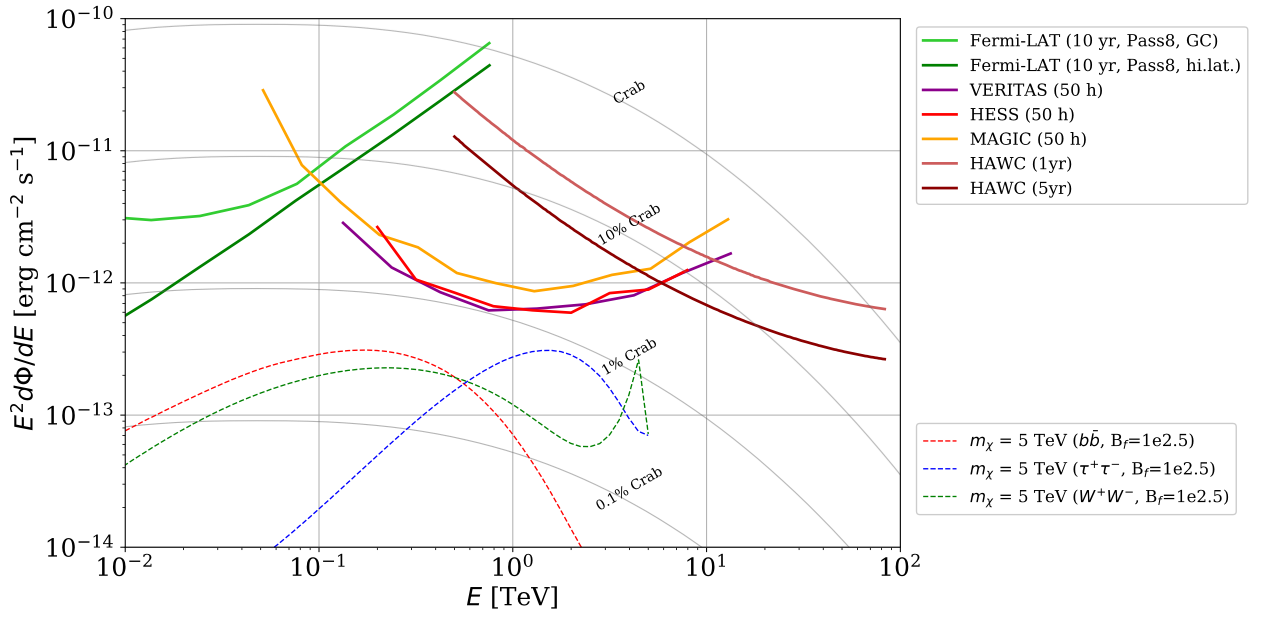
\includegraphics[scale=0.35]{figures/glory_duck/gd_motivation.png}
    }
    \caption{\ns Sensitivities of five gamma-ray experiments compared to percentages of the Crab nebula's emission and dark matter annihilation. Solid lines present estimated sensitivities to power law spectra \fu for each experiment. Green lines are Fermi-LAT sensitivities where lighter green is the sensitivity to the galactic center and light green is its sensitivity to higher declinations. Orange, red, and purple solid lines represent the MAGIC, HESS, and VERITAS 50 hour sensitivities respectively. The maroon and brown lines are the HAWC 1 year and 5 year sensitivities. Across four decades of gamma-ray energy, these experiments have similar sensitivities on the order $10^{-12}$ erg cm$^{-2}$s$^{-1}$. The dotted lines are estimated dark matter fluxes assuming DM annhilating to bottom quarks (red), tau leptons (blue), and W bosons (green). Faded grey lines outline percentage flux of the Crab nebula.}
    \label{fig:gd_motivation}
\end{figure}

Each of the five experiments featured in \Cref{fig:gd_motivation} have independently searched for DM annihilation from dwarf galaxies and set limits.
Intriguingly, their similarities overlap in regions where these observatories are less sensitive.
This clearly motivates an analysis that combines data from these five.
Each experiment has unique gammma-ray detection methods and their weaknesses and strengths can be leveraged with each other.
The HAWC gamma-ray observatory is extensively introduced in \Cref{sec:hawc}, so it is not introduced here.
A brief description of the remaining experiments are in the following paragraphs.

The Large Area Telescope (LAT) is a pair conversion telescope mounted on the NASA Fermi satellite in orbit ~550 km above the Earth \cite{FermiLAT}.
LAT's field of view covers about 20\% of the whole sky, and it sweeps the whole sky every 3 hours, approximately.
LAT's gamma-ray energy sensitivity ranges from 20 MeV up to 1 TeV.
Previous DM searches towards dwarf galaxies using Fermi-LAT are published in \cite{FermiLAT:dm1} and \cite{FermiLAT:dm2}

\sloppy The High Energy Spectroscopic System (HESS), Major Atmospheric Gamma Imaging
Cherenkov (MAGIC), and Very Energetic Radiation Imaging Telescope Array System (VERITAS) are arrays of Imaging Atmospheric Cherenkov Telescopes (IACT).
These telescopes observe the Cherenkov light emmitted from gamma-ray showers in the Earth's atmosphere.
The field for these telescopes is no larger than $5\degree$ with energy sensitivities ranging from ~ 30 GeV up to 100 TeV. \cite{HESS,MAGIC,VERITAS}
IACTs are able to make precise observations in selected regions of the sky, however can only be operated in ideal dark conditions.
HESS's  observations of the dwarves Sculptor and Carina were between January 2008 and December 2009.
HESS observations of Coma Berenices were from 2010 to 2013, and Fornax was observed in 2010 \cite{HESS:dm_sculptor_carina,HESS:dm_dwarves,HESS:dm_gamma_lines}.
MAGIC provided deep observations of Segue1 between 2011 and 2013 \cite{MAGIC:dm_segue1}.
MAGIC also provides data for three dwarves: Coma Berenices, Draco, and Ursa Major II where observations were made in: January - June 2019 \cite{MAGIC:dm_comab_draco}, March - September 2018 \cite{MAGIC:dm_comab_draco}, and 2014 - 2016 \cite{MAGIC:dm_uma2} respectively.
VERITAS provided data for Boötes I, Draco, Segue 1, and Ursa Minor from 2009 to 2016 \cite{VERITAS:dm_dwarves}

This chapter presents the Glory Duck analysis, the name given for the search for dark matter annihilation from dwarf galaxies by combining data from the five gamma-ray observatories: Fermi-LAT, HAWC, HESS, MAGIC, and VERITAS.
Specifically, the methods in analysis and modeling are presented for the HAWC gamma-ray observatory.
This work was published to ??? and presented at the International Cosmic Ray Conferance in 2019, 2021, and 2023 \cite{glory_duck:ICRC2019,glory_duck:ICRC2021,glory_duck:ICRC2023} and more.

%%%%%%%%%%%%%%%%%%%%%%%%%%%%%%%%%%%%%%%%%%%%%%%%%%%%%%%%%%%%%%%%%%%%%%%%%%%%%%%%%%%%%
\section{Dataset and Background \label{sec:gd_databgd}}
%%%%%%%%%%%%%%%%%%%%%%%%%%%%%%%%%%%%%%%%%%%%%%%%%%%%%%%%%%%%%%%%%%%%%%%%%%%%%%%%%%%%%

This section enumerates the data and background methods used for HAWC's study of the dwarf spheroidal galaxies (dSph).
\Cref{sec:gd_data} and \Cref{sec:gd_tools} are most useful for fellow HAWC collaborators looking to replicate the Glory Duck analisys.

%%%%%%%%%%%%%%%%%%%%%%%%%%%%%%%%%%%%%%%%%%%%%%%
\subsection{Itemized HAWC files}\label{sec:gd_data}
%%%%%%%%%%%%%%%%%%%%%%%%%%%%%%%%%%%%%%%%%%%%%%%
\begin{itemize}
    \item Detector Resolution: \url{response\_aerie\_svn\_27754\_systematics\_best\_mc\_test\_nobroadpulse\\
    \_10pctlogchargesmearing\_0.63qe\_25kHzNoise\_run5481\_curvature0\_index3.root}
    \item Data Map: \texttt{maps-20180119/liff/maptree\_1024.root}
    \item Spectral Dictionary: \texttt{DM\_CirrelliSpectrum\_dict\_gammas.npy}
    \item Analysis wiki: \url{https://private.hawc-observatory.org/wiki/index.php/Glory_Duck_Multi-Experiment_Dark_Matter_Search}
\end{itemize}

% %%%%%%%%%%%%%%%%%%%%%%%%%%%%%%%%%%%%%%%%%%%%%%%
\subsection{Software Tools and Development}\label{sec:gd_tools}
%%%%%%%%%%%%%%%%%%%%%%%%%%%%%%%%%%%%%%%%%%%%%%%

This analysis was performed using HAL and 3ML, in Python version 2\cite{Abeysekara_2017, vianello2015multimission}.
I built software to implement the \emph{Poor Particle Physicists' Cookbook} (PPPC) \cite{Cirelli_2011} DM spectral model and dSphs spatial model from \cite{Geringer_Sameth_2015} for HAWC analysis.
A NumPy version of this dictionary was made for both Py2 and Py3.
The code base for creating this dictionary is linked on my GitLab sandbox:

\begin{itemize}
    \item Py2: \href{https://gitlab.com/hawc-observatory/sandboxes/salaza82/glory-duck-hawc/-/tree/master/GD_spectrum}{Dictionary Generator (Deprecated)}
    \item Py3: \href{https://gitlab.com/hawc-observatory/sandboxes/salaza82/pppc2dict}{PPPC2Dict}
\end{itemize}

The analysis was performed using the $f_{\textrm{hit}}$ framework performed in the Crab paper\cite{Abeysekara_2017}.
The Python2 NumPy dictionary file for gamma-ray final states is \texttt{dmCirSpecDict.npy}.
The corresponding Python3 file is \texttt{DM\_CirrelliSpectrum\_dict\_gammas.npy}.
These files can also be used for decay channels and the PPPC describes how. \cite{Cirelli_2011}.
All other software used for data analysis, DM profile generation, and job submission to SLURM are also kept in my sandbox for \href{https://gitlab.com/hawc-observatory/sandboxes/salaza82/glory-duck-hawc}{the Glory Duck} project.

%%%%%%%%%%%%%%%%%%%%%%%%%%%%%%%%%%%%%%%%%%%%%%%
\subsection{Data Set and Background Description} \label{sec:gs_data_bkgd}
%%%%%%%%%%%%%%%%%%%%%%%%%%%%%%%%%%%%%%%%%%%%%%%

The HAWC data maps used for this analysis contain 1017 days of data between runs 2104 (2014-11-26) and 7476 (2017-12-20).
They were generated from pass 4.0 reconstruction.
The analysis is performed using the $f_{hit}$ energy binning scheme with bins (1-9) similar to what was done for the Crab and previous HAWC dSph analysis. \cite{Abeysekara_2017,Albert_2018}.
Bin 0 was excluded as it has substantial hadronic contamination and poor angular resolution.

This analysis was done on dwarf spheroidal (dSph) galaxies because of their large dark matter (DM) content relative to baryonic.
We consider the following to estimate the background to this study.

\begin{itemize}
    \item The dSphs are small in HAWC's field of view, so the analysis is not sensitive to large or small scale anisotropies.
    \item The dSphs used in this analysis are off the galactic plane.
    \item The dSphs are baryonically faint relative to their expected dark matter content and are not expected to contain gamma-ray sources.
\end{itemize}

Therefor we make no additional assumptions on the background from our sources and use HAWC's standard direct integration method for background estimation \cite{Abeysekara_2017}.
It is possible for gamma rays from DM annihilation to scatter in transit to HAWC via Inverse Compton Scattering (ICS).
This was investigated and its impact on the flux is basically zero.
Supporting information on this is in \Cref{sec:gd_ics}

%%%%%%%%%%%%%%%%%%%%%%%%%%%%%%%%%%%%%%%%%%%%%%%%%%%%%%%%%%%%%%%%%%%%%%%%%%%%%%%%%%%%%
\section{Analysis}\label{sec:gd_analysis}
%%%%%%%%%%%%%%%%%%%%%%%%%%%%%%%%%%%%%%%%%%%%%%%%%%%%%%%%%%%%%%%%%%%%%%%%%%%%%%%%%%%%%

The expected differential photon flux from DM-DM annihilation to standard model
particles over solid angle is described by the familiar equation.
\iddmannilation[\gamma]

Where \sv~is the velocity weighted annihilation cross-section.
$\frac{dN}{dE}$ is the expected differential number of photons produced at each energy per annihilation.
$M_\chi$ is the rest mass of the supposed DM particle.
$J$ is the astrophysical J-factor and is defined as
\jfactor

$\rho_{\chi}$ is the DM density.
How each component is generated and considered for HAWC's analysis is presented in the following sections.

%%%%%%%%%%%%%%%%%%%%%%%%%%%%%%%%%%%%%%%%%%%%%%%%%%
\subsection{$\frac{dN_\gamma}{dE_\gamma}$ - Particle Physics Component}\label{sec:gd_particlephysics}
%%%%%%%%%%%%%%%%%%%%%%%%%%%%%%%%%%%%%%%%%%%%%%%%%%

For this value, we import the PPPC with Electro-Weak (EW) corrections \cite{Cirelli_2011}.
The spectrum is implemented as a model script in astromodels for 3ML.
The PPPC model selected for this analysis included EW corrections.
The EW corrections were previously not considered for HAWC and are significant for DM annihilating to EW coupled SM particles such as all leptons, and the $\gamma$, $Z$, and $W$ bosons. \cite{Albert_2018}.
\Cref{fig:ew_vs_noew} demonstrates the significance of EW corrections for W boson annihilation.
Tables from the PPPC were reformatted into python Numpy dictionaries for collaboration-wide use.
A class in atromodels was created to include the EW correction from the PPPC and is aptly named \texttt{PPPCSpectra} within \texttt{DM\_models.py}.


\begin{figure}
\centering{
    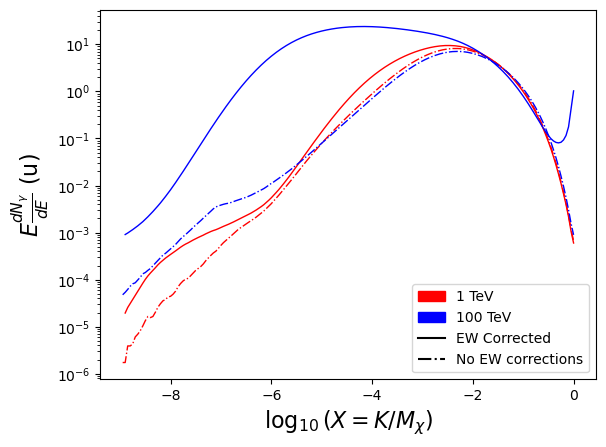
\includegraphics[scale=0.8]{figures/glory_duck/EW_vs_NoEW.png}
}
\caption{Effect of Electro-Weak (EW) corrections on expected DM annihilation spectrum for $\chi\chi \rightarrow W^-W^+$. Solid lines are spectral models that consider EW corrections. Dash-dot lines are spectral models without EW corrections. Red lines are models for $M_\chi = 1$ TeV. Blue lines represent models for $M_\chi = 100$ TeV. All models are sourced from the PPPC4DMID \cite{Cirelli_2011}.}
\label{fig:ew_vs_noew}
\end{figure}

%%%%%%%%%%%%%%%%%%%%%%%%%%%%%%%%%%%%%%%%%%%%%%%%%%
\subsection{\J - Astrophysical Component}\label{sec:gd_spatialmodel}
%%%%%%%%%%%%%%%%%%%%%%%%%%%%%%%%%%%%%%%%%%%%%%%%%%

The J-factor profiles for each source are imported from Geringer-Sameth (\GS) \cite{Geringer_Sameth_2015}.
These were provided from the authors as $\J(\theta)$, where $\theta$ is the angular separation from the center of the source.
HAWC requires maps in terms of $\frac{d\J}{d\Omega}$, so the conversion from the maps was done in the following way.

First, convert the angular distances to solid angles
\angleTOsolidangle
which reduces with a small angle approximation to $\pi \theta^2$.
Next, the central difference for both the $\Delta \J$ and $\Delta \theta$ value were calculated for the discretized form of $\J(\theta)$ with the central difference stencil:
\centerDiff
Where $\phi$ is either $\theta$ or \J.
These were done separately in case the grid spacing in $\theta$~was not uniform.
Finally, these lists are divided so that we are left with approximation of the profile of $d\J/d\Omega$~that is a function of $\theta$.
Admittedly, this is an approximation method for the map which introduces small errors compared to the true profile estimate.
This was checked as a systematic against the author's profiling of the spatial distribution and is documented in \todo{Model dependant limit, remember the jfactors!}

With $\frac{d\J}{d\Omega}$, a map is generated, first by filling in the north-east quadrant of the map.
This quadrant is then reflected twice, vertically then horizontally, to fill the full map.
Maps are then normailized by dividing the discrete 2D integral of the map.
The 2D integral was a simple height of bins, Newton's integral:
\newtonIntegral
These maps are HEALpix maps with NSIDE 16384 and saved in the \texttt{.fits} format.

\begin{figure}
    \centering{
    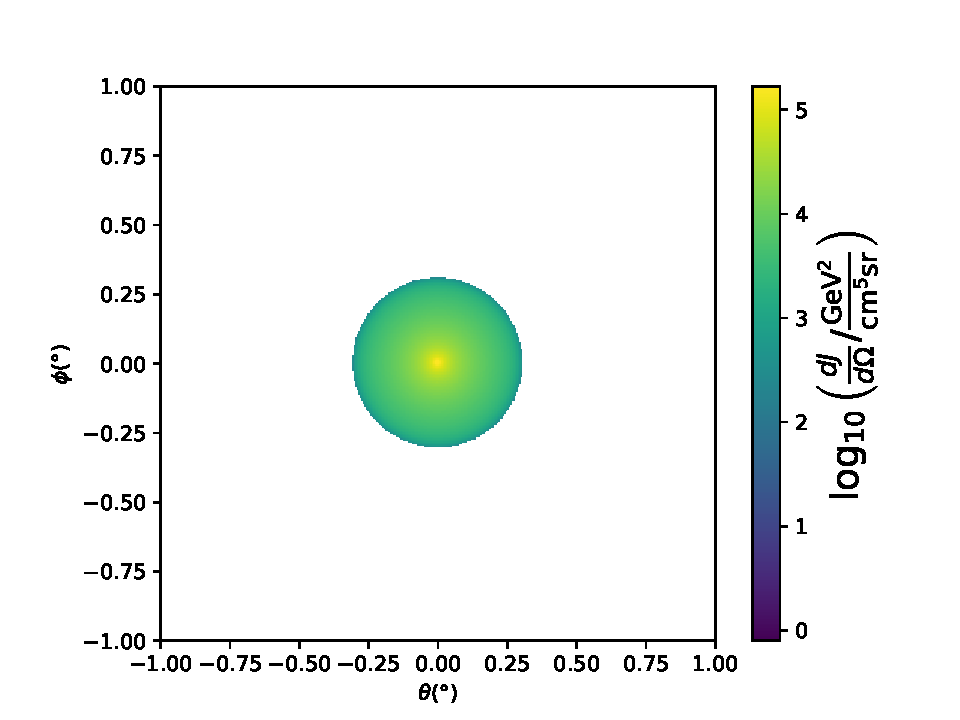
\includegraphics[scale=0.86]{figures/glory_duck/hawc/Segue1_J_plot.pdf}
    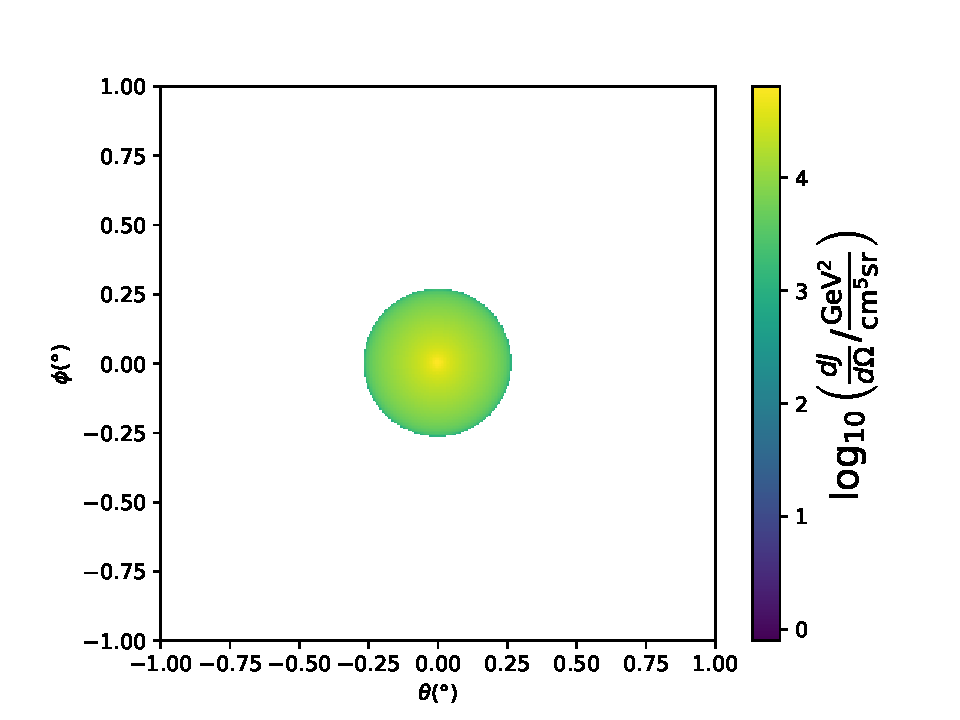
\includegraphics[scale=0.86]{figures/glory_duck/hawc/ComaBerenices_J_plot.pdf}
    }
    \caption{$\frac{d\J}{d\Omega}$ maps for Segue1 (top) and Coma Berenices (bottom). Origin is centered on the specific dwarf spheroidal galaxies (dSph). X and Y axes are the angular separation from the center of the dwarf. Plots of the remaining 11 dSph HAWC studied are linked in \Cref{sec:gd_tools}.}\label{fig:gd_spatialmodel}
\end{figure}

Another DM spatial distribution model from Bonnivard (\B) \cite{Bonnivard:2014kza} was used for the complete study.
However, to save computational time, limits from \GS were scaled to \B instead of each experiment performing a full study a second time.
How these models compare is demonstrated for each dSph in \Cref{fig:comparison_J_1} and \Cref{fig:comparison_J_2}
Plots of these maps are provided for each source in the sandbox directory: \texttt{GD\_mass\_profiles}.
Examples of the two most impactful dSphs, Segue1 and Coma Berenices are featured in \Cref{fig:gd_spatialmodel}

%%%%%%%%%%%%%%%%%%%%%%%%%%%%%%%%%%%%%%%%%%%%%%%%%%
\subsection{Source Selection and Annihilation Channels}\label{sec:gd_srcs_y_chan}
%%%%%%%%%%%%%%%%%%%%%%%%%%%%%%%%%%%%%%%%%%%%%%%%%%

We use many of the dSph presented in our previous dSph DM search \cite{Albert_2018}.
HAWC's sources for Glory Duck include Boötes I, Coma Berenices, Canes Venatici I + II, Draco, Hercules, Leo I, II, + IV, Segue 1, Sextans, and Ursa Major I + II.
A full description of all sources used in Glory Duck is found in \Cref{tab:gd_J_factor}.
Triangulum II was excluded from the Glory Duck analysis because of large uncertainties in its J-factor.
Ursa Minor was excluded from HAWC's contribution to the combination because the source extension model extended Ursa Minor beyond HAWC's field of view.
Ursa Minor was not expected to contribute significantly to the combined limit, so work was not invested in a solution to include Ursa Minor.

The DM annihilation channels probed for the Glory Duck combination include $b\bar{b}$, $e\bar{e}$, $\mu\bar{\mu}$, $\tau\bar{\tau}$, $t\bar{t}$, $W^+W^-$, and $ZZ$.
A summary of all sources, with a description of each experiments' sensitivity to the source, is provided in \Cref{tab:gd_tabSummary}.

\afterpage{%
    \newgeometry{margin=2.5cm} % modify this if you need even more space
    \begin{landscape}
%
\vspace*{\fill}
\begin{table}
\caption{Summary of dSph observations by each experiment used in this work. A `-' indicates the experiment did not observe the dSph for this study. For Fermi-LAT, the exposure at 1~GeV is given. For HAWC, $|\Delta\theta|$ is the absolute difference between the source declination and HAWC latitude. HAWC is more sensitive to sources with smaller $|\Delta\theta|$. For IACTs, we show the zenith angle range, the total exposure, the energy range, the angular radius $\theta$  of the signal or ON region, the ratio of exposures between the background-control (OFF) and signal (ON) regions ($\tau$), and the significance of gamma-ray excess in standard deviations, $\sigma$.}
\centering
{\begin{tabular}{c ? c ? c ? c c c c c c c }
\hline
\hline
& \multicolumn{1}{c?}{Fermi-LAT}  & \multicolumn{1}{c?}{HAWC} & \multicolumn{7}{c}{H.E.S.S, MAGIC, VERITAS} \\
\hline
Source name & Exposure ($10^{11}$ s m$^2$) & $|\Delta\theta|$ (\degree) & IACT & Zenith (\degree) & Exposure (h) & Energy range (GeV) & $\theta$ (\degree) & $\tau$ & S ($\sigma$) \\
\hline\hline
Bo\"{o}tes I            & $2.6$ & $4.5$ & VERITAS  & $15-30$ & $14.0$ & $100 $-$ 41000$ & $0.10$ & $8.6$ & $-1.0$  \\
Canes Venatici I        & $2.9$ & $14.6$ & $-$ & $-$ & $-$ & $-$ & $-$ & $-$ & $-$  \\
Canes Venatici II       & $2.9$ & $15.3$ & $-$ & $-$ & $-$ & $-$ & $-$ & $-$ & $-$  \\
Carina                  & $3.1$ & $-$ & H.E.S.S. & $27-46$ & $23.7$ & $310 - 70000$ & $0.10$ & $18.0$ & $-0.3$  \\
\hdashline
\multirow{2}{*}{Coma Berenices}          & \multirow{2}{*}{$2.7$} & \multirow{2}{*}{$4.9$} & H.E.S.S. & $47-49$ & $11.4$ & $550 - 70000$ & $0.10$ & $14.4$ & $-0.4$  \\
                                         & & & MAGIC & $5 - 37 $ & $49.5$ & $60 - 10000$ & $0.17$ & $1.0$ & $-$\\
\hdashline
\multirow{2}{*}{Draco}                   & \multirow{2}{*}{$3.8$} & \multirow{2}{*}{$38.1$} & MAGIC & $29 - 45$ & $52.1$ & $70 - 10000$ & $0.22$ & $1.0$ & $-$  \\
                                         & & & VERITAS & $25-40$ & $49.8$ & $120 - 70000$ & $0.10$ & $9.0$ & $-1.0$ \\
\hdashline
Fornax                  & $2.7$ & $-$ & H.E.S.S. & $11-25$ & $6.8$ & $230 - 70000$ & $0.10$ & $45.5$ & $-1.5$ \\
Hercules                & $2.8$ & $6.3$ & $-$ & $-$ & $-$ & $-$ & $-$ & $-$ & $-$  \\
Leo I                   & $2.5$ & $6.7$ & $-$ & $-$ & $-$ & $-$ & $-$ & $-$ & $-$  \\
Leo II                  & $2.6$ & $3.1$ & $-$ & $-$ & $-$ & $-$ & $-$ & $-$ & $-$  \\
Leo IV                  & $2.4$ & $19.5$ & $-$ & $-$ & $-$ & $-$ & $-$ & $-$ & $-$ \\
Leo V                   & $2.4$ & $-$ & $-$ & $-$ & $-$ & $-$ & $-$ & $-$ & $-$  \\
Leo T                   & $2.6$ & $-$ & $-$ & $-$ & $-$ & $-$ & $-$ & $-$ & $-$  \\
Sculptor                & $2.7$ & $-$ & H.E.S.S. & $10-46$ & $11.8$ & $200 - 70000$ & $0.10$ & $19.8$ & $-2.2$  \\
\hdashline
\multirow{2}{*}{Segue I}& \multirow{2}{*}{$2.5$} & \multirow{2}{*}{$2.9$} & MAGIC & $13-37$ & $158.0$ & $60 - 10000$ & $0.12$ & $1.0$ & $-0.5$ \\
                        & & & VERITAS & $15-35$ & $92.0$ & $80 - 50000$ & $0.10$ & $7.6$ & $0.7$ \\
\hdashline
Segue II                & $2.7$ & $-$ & $-$ & $-$ & $-$ & $-$ & $-$ & $-$ & $-$ \\
Sextans                 & $2.4$ & $20.6$ & $-$ & $-$ & $-$ & $-$ & $-$ & $-$ & $-$  \\
Ursa Major I            & $3.4$ & $32.9$ & $-$ & $-$ & $-$ & $-$ & $-$ & $-$ & $-$  \\
Ursa Major II           & $4.0$ & $44.1$ & MAGIC & $35-45$ & $94.8$ & $120 - 10000$ & $0.30$ & $1.0$ & $-2.1$  \\
Ursa Minor              & $4.1$ & $-$ &  VERITAS & $35-45$ & 60.4 & $160-93000$ & 0.10 & 8.4 & $-0.1$ \\
\hline
\end{tabular}}
\label{tab:tabSummary}
\end{table}
\vspace*{\fill}
%
\end{landscape}
\restoregeometry
}
%

\begin{table}[h!]
% \captionsetup{font=small}
\centering
    \caption{Summary of the relevant properties of the dSphs used in the present work. Column 1 lists the dSphs. Columns 2 and 3 present their heliocentric distance and galactic coordinates, respectively. Columns 4 and 5 report the \J-factors of each source given from the \GS and \B independent studies and their estimated $\pm 1\sigma$ uncertainties. The values $\log_{10}J$~(\GS set) \cite{Geringer_Sameth_2015} correspond to the mean \J-factor values  for a source extension truncated at the outermost observed star. The values $\log_{10}J$~(\B set) \cite{Bonnivard:2014kza} are provided for a source extension at the tidal radius of each dSph. \textbf{Bolded sources are within HAWC's field of view and provided to the Glory Duck analysis.}}
    {\begin{tabular}{ccccc}
    \hline
    \hline
    \CellTopTwo{}
    Name & Distance & $l, b$ & $\log_{10}J$~(\GS set) & $\log_{10}J$~(\B set)\\
    & \scriptsize{(kpc)} &  \scriptsize{($\degree$)} & \scriptsize{$\log_{10}(\mathrm{GeV}^2 \mathrm{cm}^{-5}\mathrm{sr})$} & \scriptsize{$\log_{10}(\mathrm{GeV}^2 \mathrm{cm}^{-5}\mathrm{sr})$}  \\
    \hline
    \CellTopTwo{}
    \textbf{Bo\"otes} I & $66$ & $358.08,\: 69.62$ & $18.24^{+0.40}_{-0.37}$ & $18.85^{+1.10}_{-0.61}$  \\
    \CellTopTwo{}
    \textbf{Canes Venatici I} & $218$ & $74.31,\: 79.82$ & $17.44^{+0.37}_{-0.28}$ & $17.63^{+0.50}_{-0.20}$  \\
    \CellTopTwo{}
    \textbf{Canes Venatici II} & $160$ & $113.58,\: 82.70$ & $17.65^{+0.45}_{-0.43}$ & $18.67^{+1.54}_{-0.97}$  \\
    \CellTopTwo{}
    Carina & $105$ & $260.11,\: -22.22$ & $17.92^{+0.19}_{-0.11}$ & $18.02^{+0.36}_{-0.15}$ \\
    \CellTopTwo{}
    \textbf{Coma Berenices} & $44$ & $241.89,\: 83.61$ & $19.02^{+0.37}_{-0.41}$ & $20.13^{+1.56}_{-1.08}$  \\
    \CellTopTwo{}
    \textbf{Draco} & $76$ & $86.37,\: 34.72$ & $19.05^{+0.22}_{-0.21}$ &  $19.42^{+0.92}_{-0.47}$  \\
    \CellTopTwo{}
    Fornax & $147$ & $237.10,\: -65.65$ & $17.84^{+0.11}_{-0.06}$ &  $17.85^{+0.11}_{-0.08}$  \\
    \CellTopTwo{}
    \textbf{Hercules} & $132$ & $28.73,\: 36.87$ & $16.86^{+0.74}_{-0.68}$ &  $17.70^{+1.08}_{-0.73}$  \\
    \CellTopTwo{}
    \textbf{Leo I} & $254$ & $225.99,\: 49.11$ & $17.84^{+0.20}_{-0.16}$ &  $17.93^{+0.65}_{-0.25}$  \\
    \CellTopTwo{}
    \textbf{Leo II} & $233$ & $220.17,\: 67.23$ & $17.97^{+0.20}_{-0.18}$ &  $18.11^{+0.71}_{-0.25}$  \\
    \CellTopTwo{}
    \textbf{Leo IV} & $154$ & $265.44,\: 56.51$ & $16.32^{+1.06}_{-1.70}$ & $16.36^{+1.44}_{-1.65}$  \\
    \CellTopTwo{}
    Leo V & $178$ & $261.86,\: 58.54$ & $16.37^{+0.94}_{-0.87}$ & $16.30^{+1.33}_{-1.16}$  \\
    \CellTopTwo{}
    Leo T & $417$ & $214.85,\: 43.66$ & $17.11^{+0.44}_{-0.39}$ & $17.67^{+1.01}_{-0.56}$  \\
    \CellTopTwo{}
    Sculptor & $86$ & $287.53,\: -83.16$ & $18.57^{+0.07}_{-0.05}$ &  $18.63^{+0.14}_{-0.08}$  \\
    \CellTopTwo{}
    \textbf{Segue I} & $23$ & $220.48,\: 50.43$ & $19.36^{+0.32}_{-0.35}$ &  $17.52^{+2.54}_{-2.65}$  \\
    \CellTopTwo{}
    Segue II & $35$ & $149.43,\: -38.14$ & $16.21^{+1.06}_{-0.98}$ & $19.50^{+1.82}_{-1.48}$  \\
    \CellTopTwo{}
    \textbf{Sextans} & $86$ & $243.50,\: 42.27$ & $17.92^{+0.35}_{-0.29}$ &  $18.04^{+0.50}_{-0.28}$  \\
    \CellTopTwo{}
    \textbf{Ursa Major I} & $97$ & $159.43,\: 54.41$ & $17.87^{+0.56}_{-0.33}$ & $18.84^{+0.97}_{-0.43}$  \\
    \CellTopTwo{}
    \textbf{Ursa Major II} & $32$ & $152.46,\: 37.44$ & $19.42^{+0.44}_{-0.42}$ & $20.60^{+1.46}_{-0.95}$  \\
    \CellTopTwo{}
    Ursa Minor & $76$ & $104.97,\: 44.80$ & $18.95^{+0.26}_{-0.18}$ & $19.08^{+0.21}_{-0.13}$  \\
    \hline
    \hline
    \CellTopTwo{}
\end{tabular}} \label{tab:gd_J_factor}
\end{table}

%%%%%%%%%%%%%%%%%%%%%%%%%%%%%%%%%%%%%%%%%%%%%%%%%%%%%%%%%%%%%
\subsection{Likelihood Methods} \label{sec:gd_ll_methods}
%%%%%%%%%%%%%%%%%%%%%%%%%%%%%%%%%%%%%%%%%%%%%%%%%%%%%%%%%%%%%

We perform a standard HAWC binned maximum likelihood analysis using $f_{hit}$ bins 1-9.
This analysis was performed using HAL and 3ML, in Python2 \cite{Abeysekara_2017, vianello2015multimission}.
With these tools we compute the max from the likelihood profiles and perform a ratio test to calculate the significance of each source.
This analysis is identical to the previous dSph analysis \cite{Albert_2018} except the sources are treated as extended.
For the vast majority of our sources, this extension is no greater than 2 degrees.
We calculate the likelihood of each source and model, assuming events are Poisson distributed, with
\hwcpsLLH

$S_i$ is the sum of expected number of signal counts.
$B_i$ is the number of background counts observed.
$N_i$ is the total number of counts.
The \textit{i}th bin is iterated over spatial and $f_{\textrm{hit}}$.
Then we combine the profiles across all five experiments.
The profile likelihood ratio $\lambda$ as a function of annihilation cross-section \sv is computed by:
\gdLLHratio
for a considered annihilation channel and DM mass.

\todo{Section pasted from paper. Rephrase cause plagarism is a thing.}
As mentioned previously, each experiment computes the $\mathcal{L}_{lk}$ from \Cref{eq:gd_LLH_test} differently.
The remainder of this section highlights the differences in this calculation across the experiments.
Four experiments, namely \textit{Fermi}-LAT, H.E.S.S., HAWC and MAGIC, use a binned likelihood to compute the $\mathcal{L}_{lk}$.
For these experiments, for each observation $\bm{\mathcal{D}_{lk}}$ of a given dSph $l$ carried out using a given gamma-ray detector $k$, the binned likelihood function is:
\gdJointLLH

where $N_{\text{E'}}$ and $N_{\text{P'}}$ are the number of considered bins in reconstructed energy and arrival direction, respectively; $\mathcal{P}$ represents a Poisson PDF for the number of gamma-ray candidate events $ N_{lk,ij} $ observed in the $i$-th bin in energy and $j$-th bin in arrival direction, when the expected number is the sum of the expected mean number of signal events $ s_{ij} $ (produced by DM annihilation) and of background events $ b_{ij} $; $ \mathcal{L}_{lk,\bm{\nu}} $ is the likelihood term for the extra $ \bm{\nu_{lk}} $ nuisance parameters that vary from one instrument $k$ to another.
The expected counts for signal events $s_{ij}$ for a given dSph $l$ and detector $k$ is given by:

\gdExpectedNS

where $ E' $ and $ E $ are the reconstructed and true energies, $ P' $ and $ P $ the reconstructed and true arrival directions; $ E'_{\text{min},i} $, $ P'_{\text{min},j} $, $ E'_{\text{max},i} $, and $ P'_{\text{max},j} $ are their lower and upper limits of the $ i $-th energy bin and the $ j $-th arrival direction bin; $ T_{\text{obs}} $ is the (dead-time corrected) total observation time; $ t $ is the time along the observations; $ \text{d}^{2}\Phi/\text{d}E\text{d}\Omega $ is the DM flux in the source region (see \Cref{eq:id_dm_flux});
and $ \text{IRF} \left( E', P' \mid E, P, t \right) $ is the IRF, which can be factorized as the product of the effective collection area of the detector $ A_{\mathrm{eff}} (E, P, t) $, the PDFs for the energy estimator $ f_{E} (E' \mid E,t) $, and arrival direction $ f_{P} (P' \mid E,P,t) $ estimators.
Note that for Fermi-LAT, HAWC, MAGIC, and VERITAS the effect of the finite angular resolution is taken into account through the convolution of $d\Phi/dE d\Omega$ with $f_{P}$ in \Cref{eq:gd_expected_ns}, whereas in the cases of H.E.S.S. $f_{P}$ is approximated by a delta function.
This approximation has been made in order to maintain compatibility of the result with what has been previously published.
The difference introduced by this approximation is $<5\%$ for all considered dSphs.
\todo{End of paper section}

From \Cref{eq:gd_LLH_test}, we can compute the test statistic (TS) with the ratio test:

\gdTS

$\mathcal{L}^{\textrm{max}}$ here is equivalent to $\mathcal{L}(N_i, B_i,S_i=0)$ or no signal counts.

\begin{figure}
\centering{
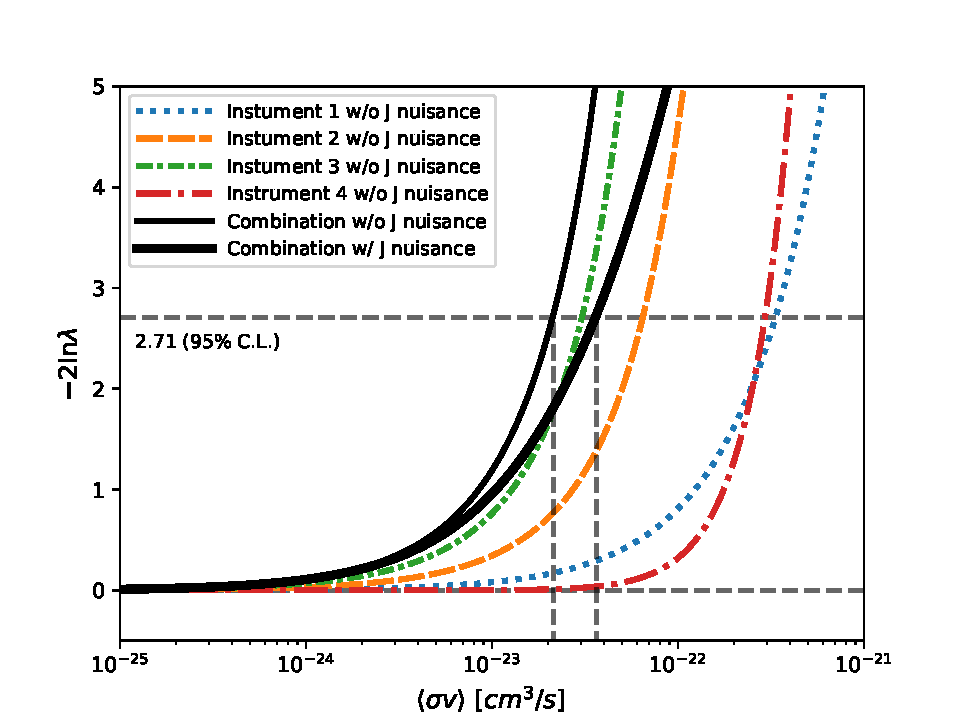
\includegraphics[width=0.7\textwidth]{figures/glory_duck/comparison/Combined_exp_technique_20TeV_4exp_J_with_without_nuisance_v2.pdf}}
\caption{Illustration of the combination technique showing a comparison between $-2\ln  \lambda$ provided by four instruments (colored lines) from the observation of the same dSph without any \J nuisance and their sum, $i.e.$ the resulting combined likelihood (thin black line). According to the test statistics of \Cref{eq:gd_TS}, the intersection of the likelihood profiles with the line $-2\ln  \lambda$ = 2.71 indicates the 95\% C.L. upper limit on \sv. The combined likelihood (thin black line) shows a smaller value of upper limit on $\langle \sigma v \rangle$ than those derived by individual instruments. We also show the uncertainties on the \J-factor affects the combined likelihood and degrade the upper limit on \sv (thick black line). All likelihood profiles are normalized so that the global minimum $\widehat{\svtex}$ is 0. We note that each profile depends on the observational conditions in which a target object was observed. The sensitivity of a given instrument can be degraded and the upper limits less constraining if the observations are performed in non optimal conditions such as a high zenith angle or a short exposure time.}
\label{fig:illustration_combination}
\end{figure}

%%%%%%%%%%%%%%%%%%%%%%%%%%%%%%%%%%%%%%%%%%%%%%%%%%%%%%%%%%%%%
\section{HAWC Results}\label{sec:hawc_results}
%%%%%%%%%%%%%%%%%%%%%%%%%%%%%%%%%%%%%%%%%%%%%%%%%%%%%%%%%%%%%

13 of the 20 dSphs considered for the Glory Duck analysis are within HAWC's field of view.
These dSph are analyzed for emission from DM annihilation according to the likelihood method described in \Cref{sec:gd_ll_methods}.
The 13 likelihood profiles are then combined to create a combined limit on the dark matter cross-section.
This combination is done for the 7 annihilation channels used in the Glory Duck analysis.
\Cref{fig:hawc_combined_limit} shows the combined limit for all annihilation channels with HAWC only observations.
We also perform 300 studies of Poisson trials on the background.
These trials are used to produce HAWC Brazil bands which were shared with the other collaborators for combined Brazil Bands.
The results on fitting to HAWC's poisson trials of the DM hypothesis is shown in \Cref{fig:hawc_brazil_band} for seven of the DM annihilation channels.

No DM was found in HAWC observations.
The limits are dominated by the dSph Segue1 and Coma Berenices.
The remaining 11 dSphs do no contribute significantly to the limit.
Even though some of the remaining dSphs have large J-factors, they are towards the edge of HAWC's field of view where this analysis is less sensitive.

\begin{figure}[ht]
    \centering{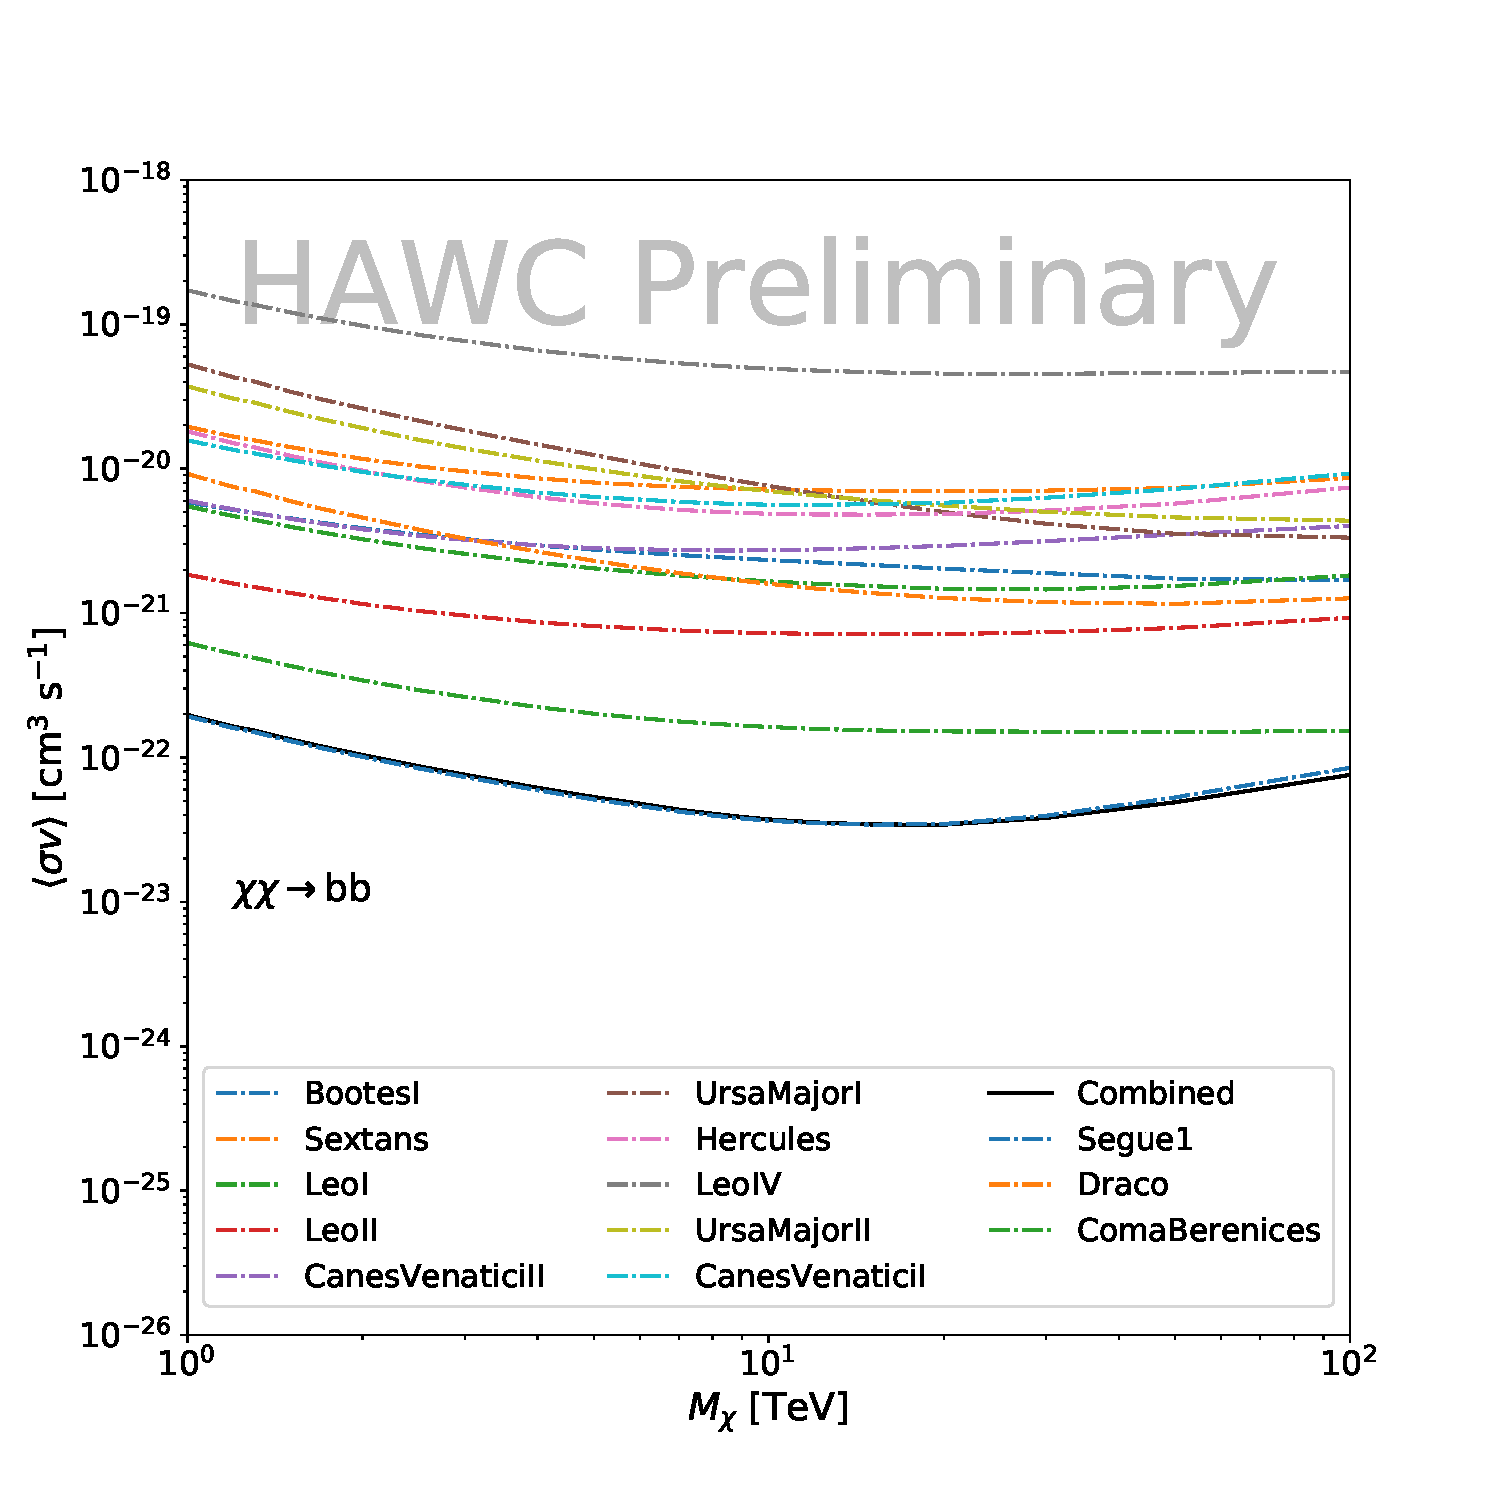
\includegraphics[scale=0.21]{figures/glory_duck/hawc/Combined95_GD_bb.pdf}
    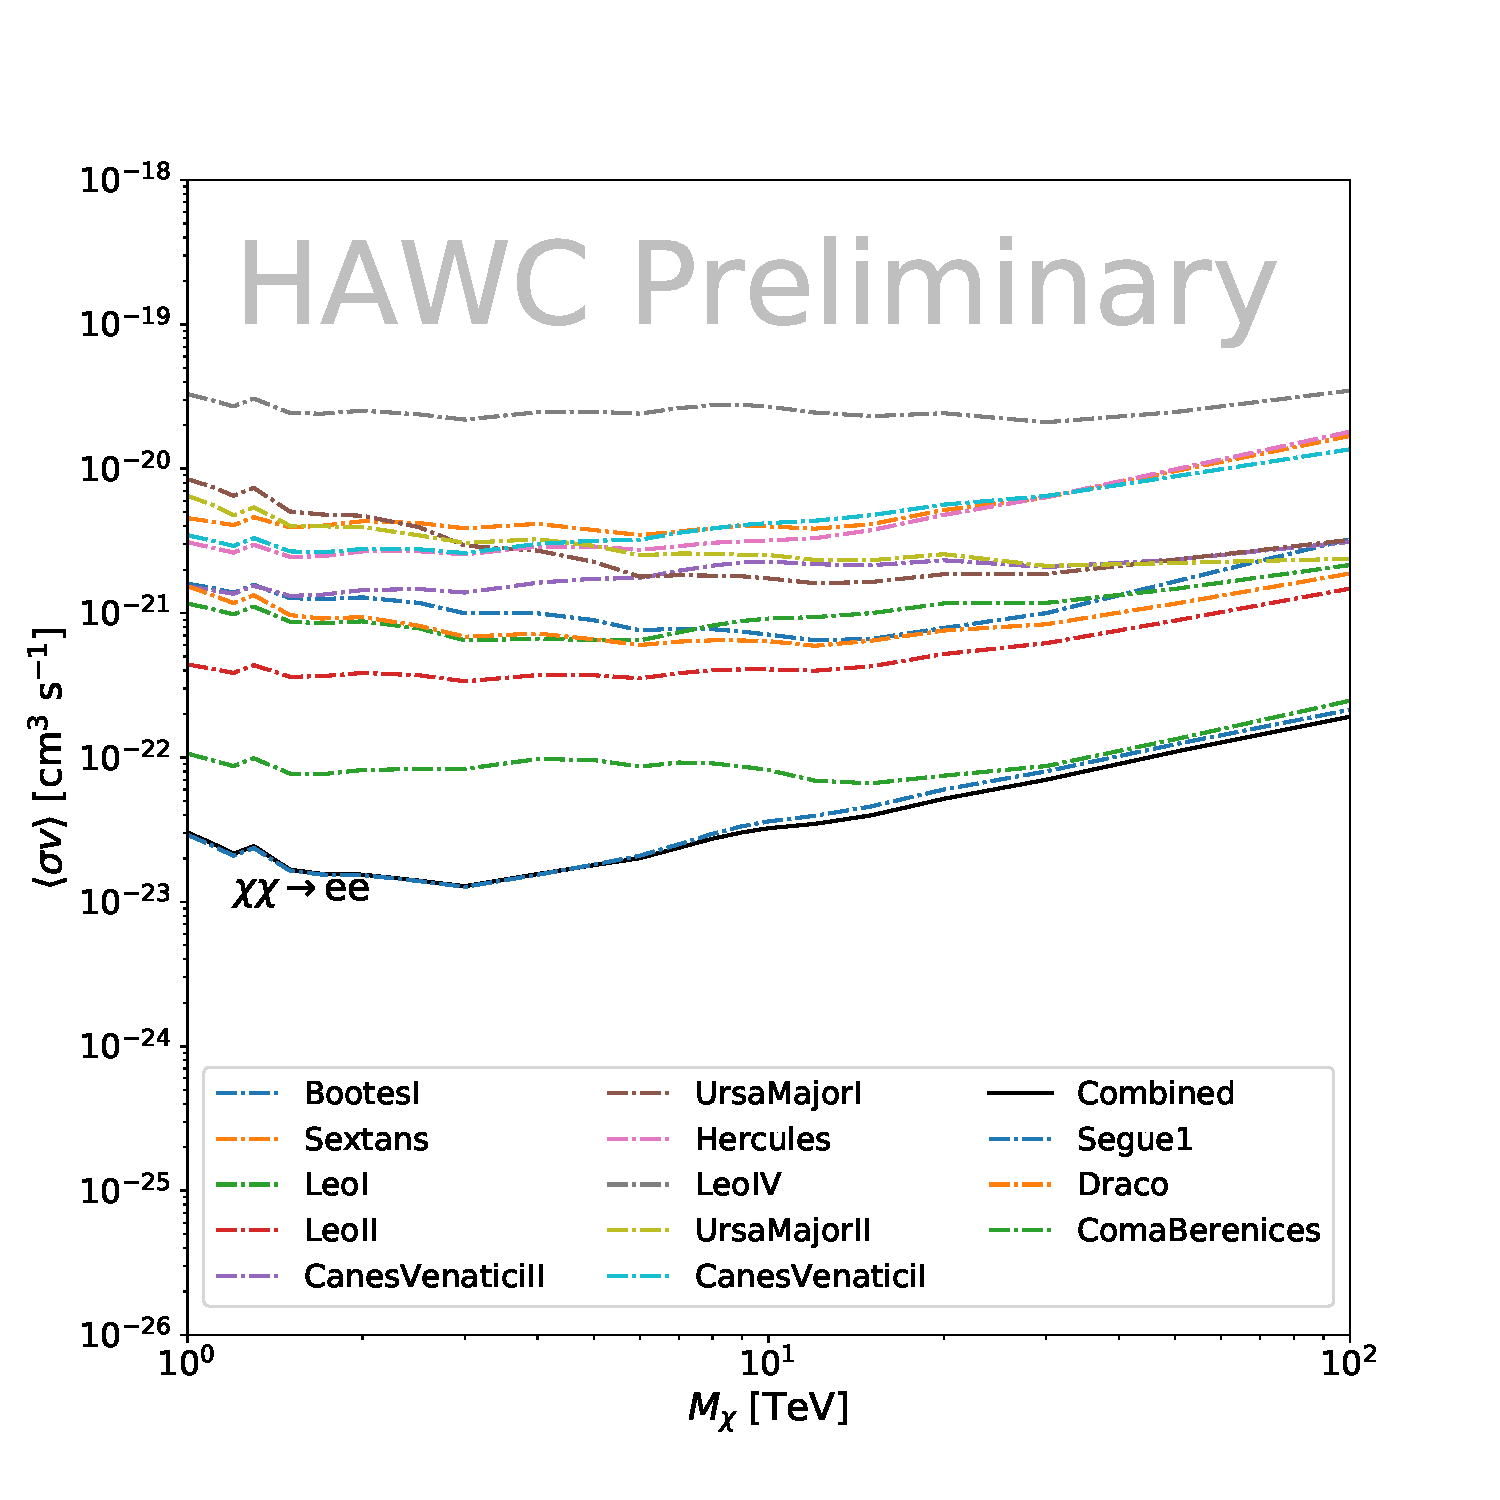
\includegraphics[scale=0.21]{figures/glory_duck/hawc/Combined95_GD_ee.pdf}
    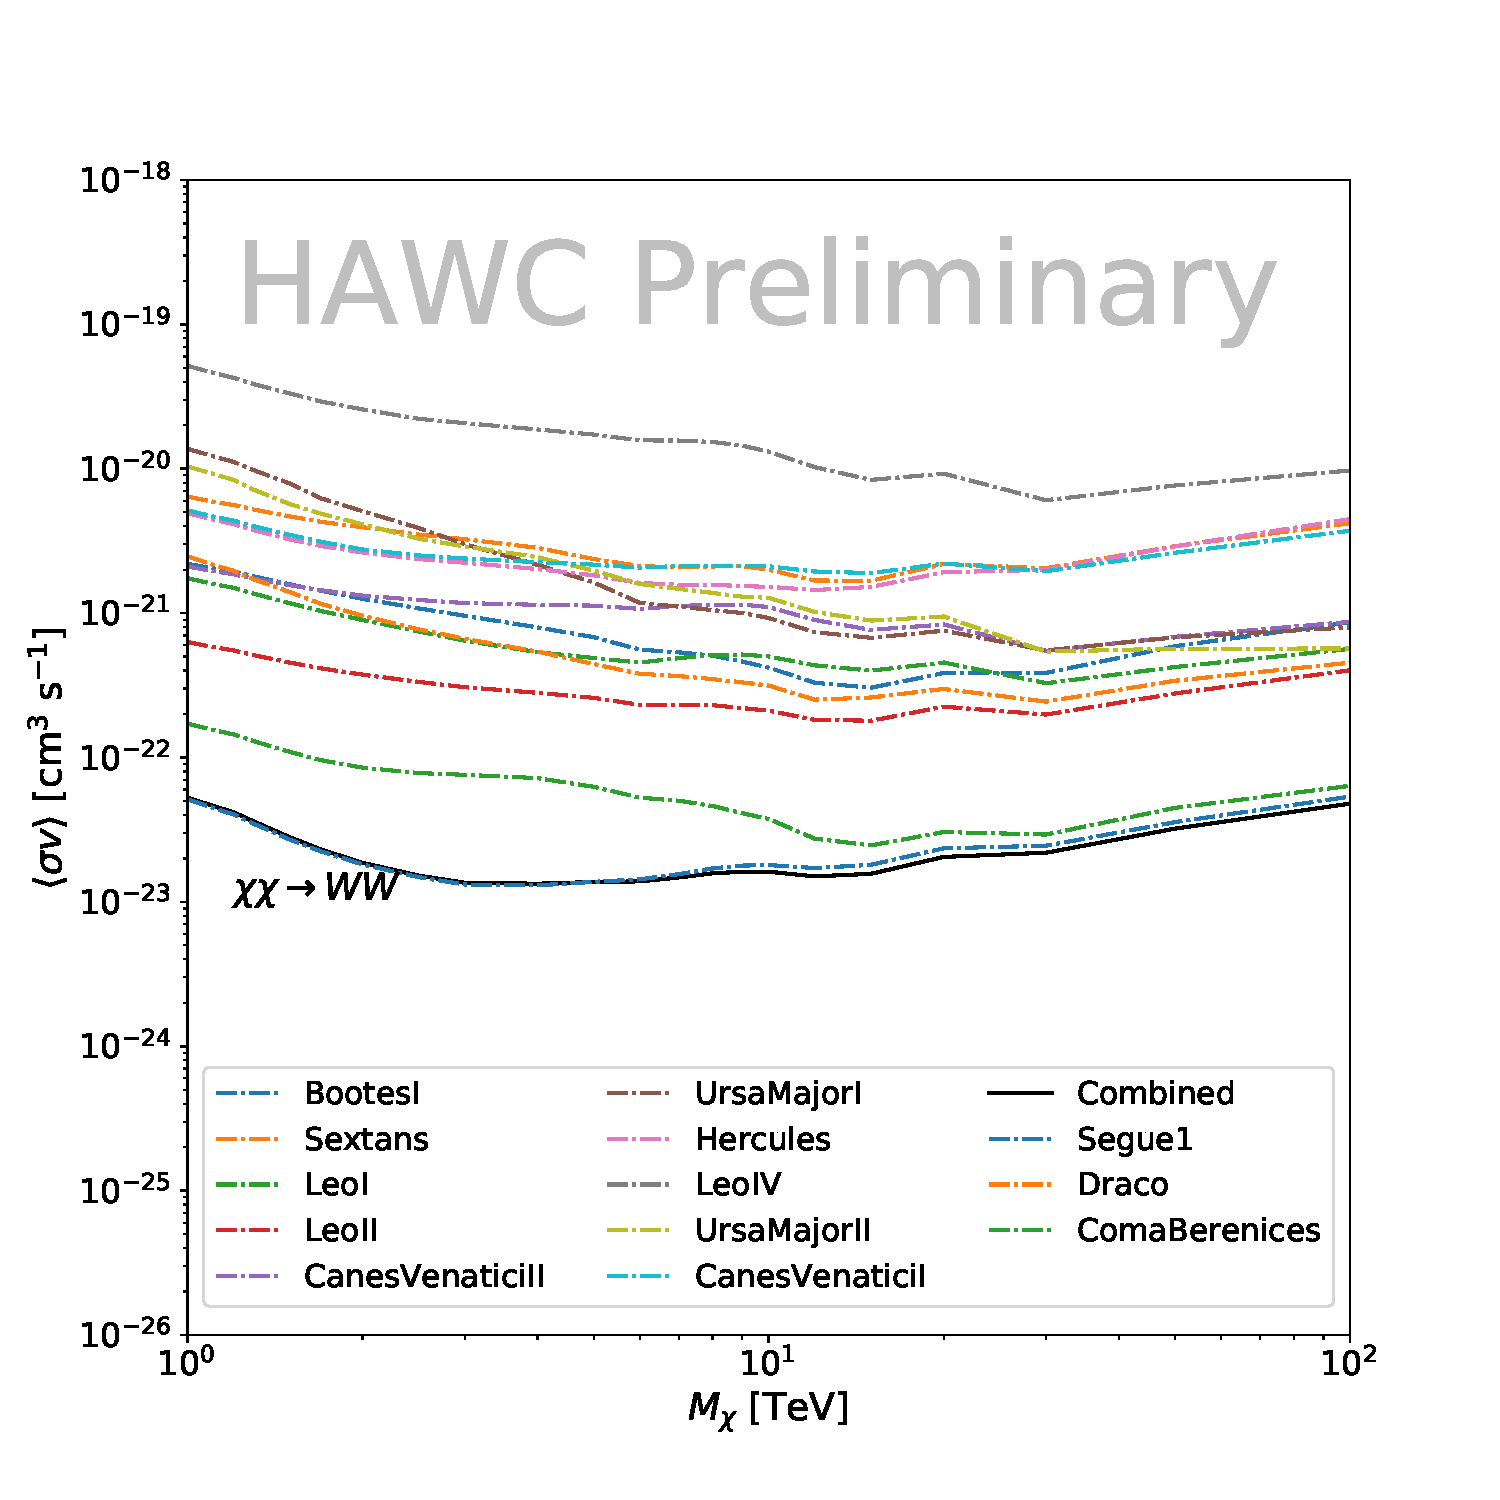
\includegraphics[scale=0.21]{figures/glory_duck/hawc/Combined95_GD_ww.pdf}
    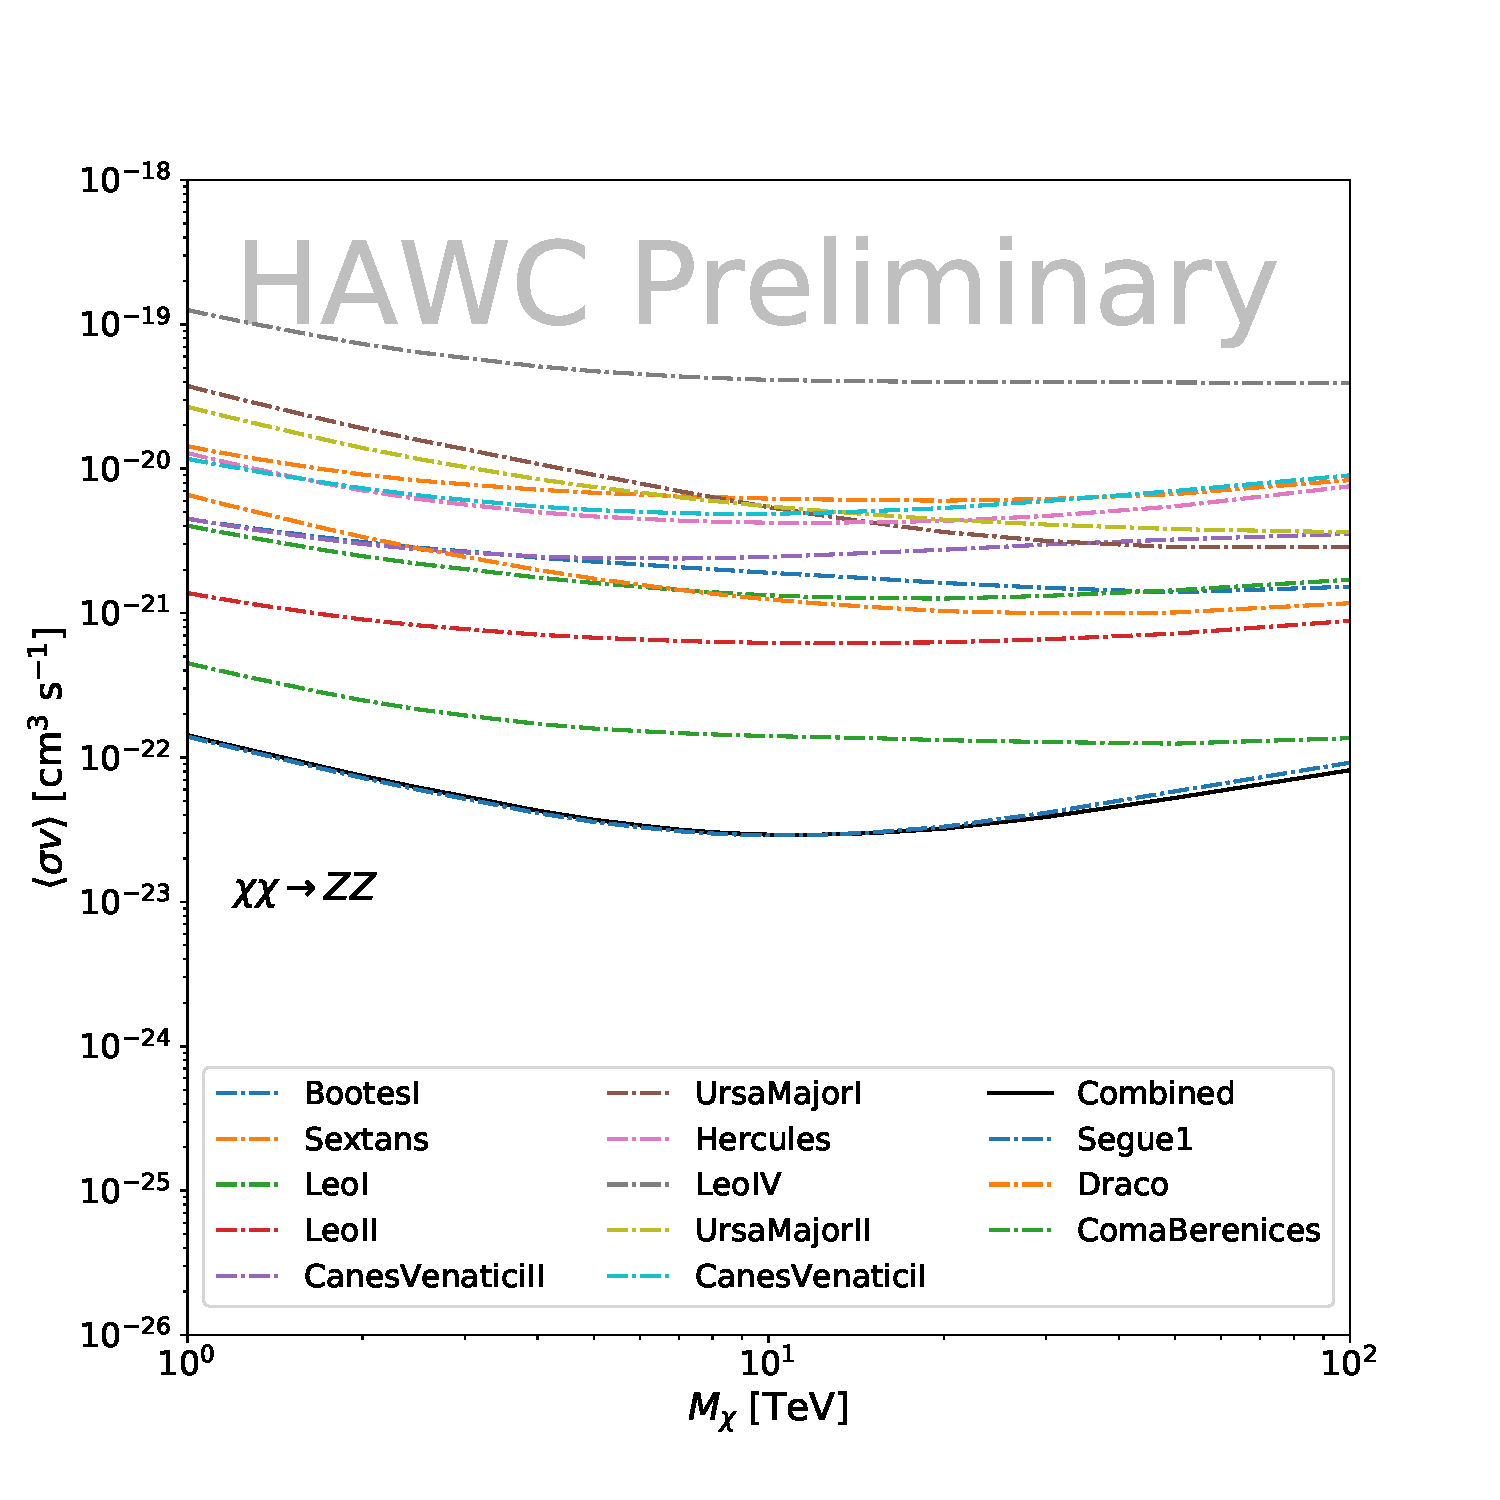
\includegraphics[scale=0.21]{figures/glory_duck/hawc/Combined95_GD_zz.pdf}
    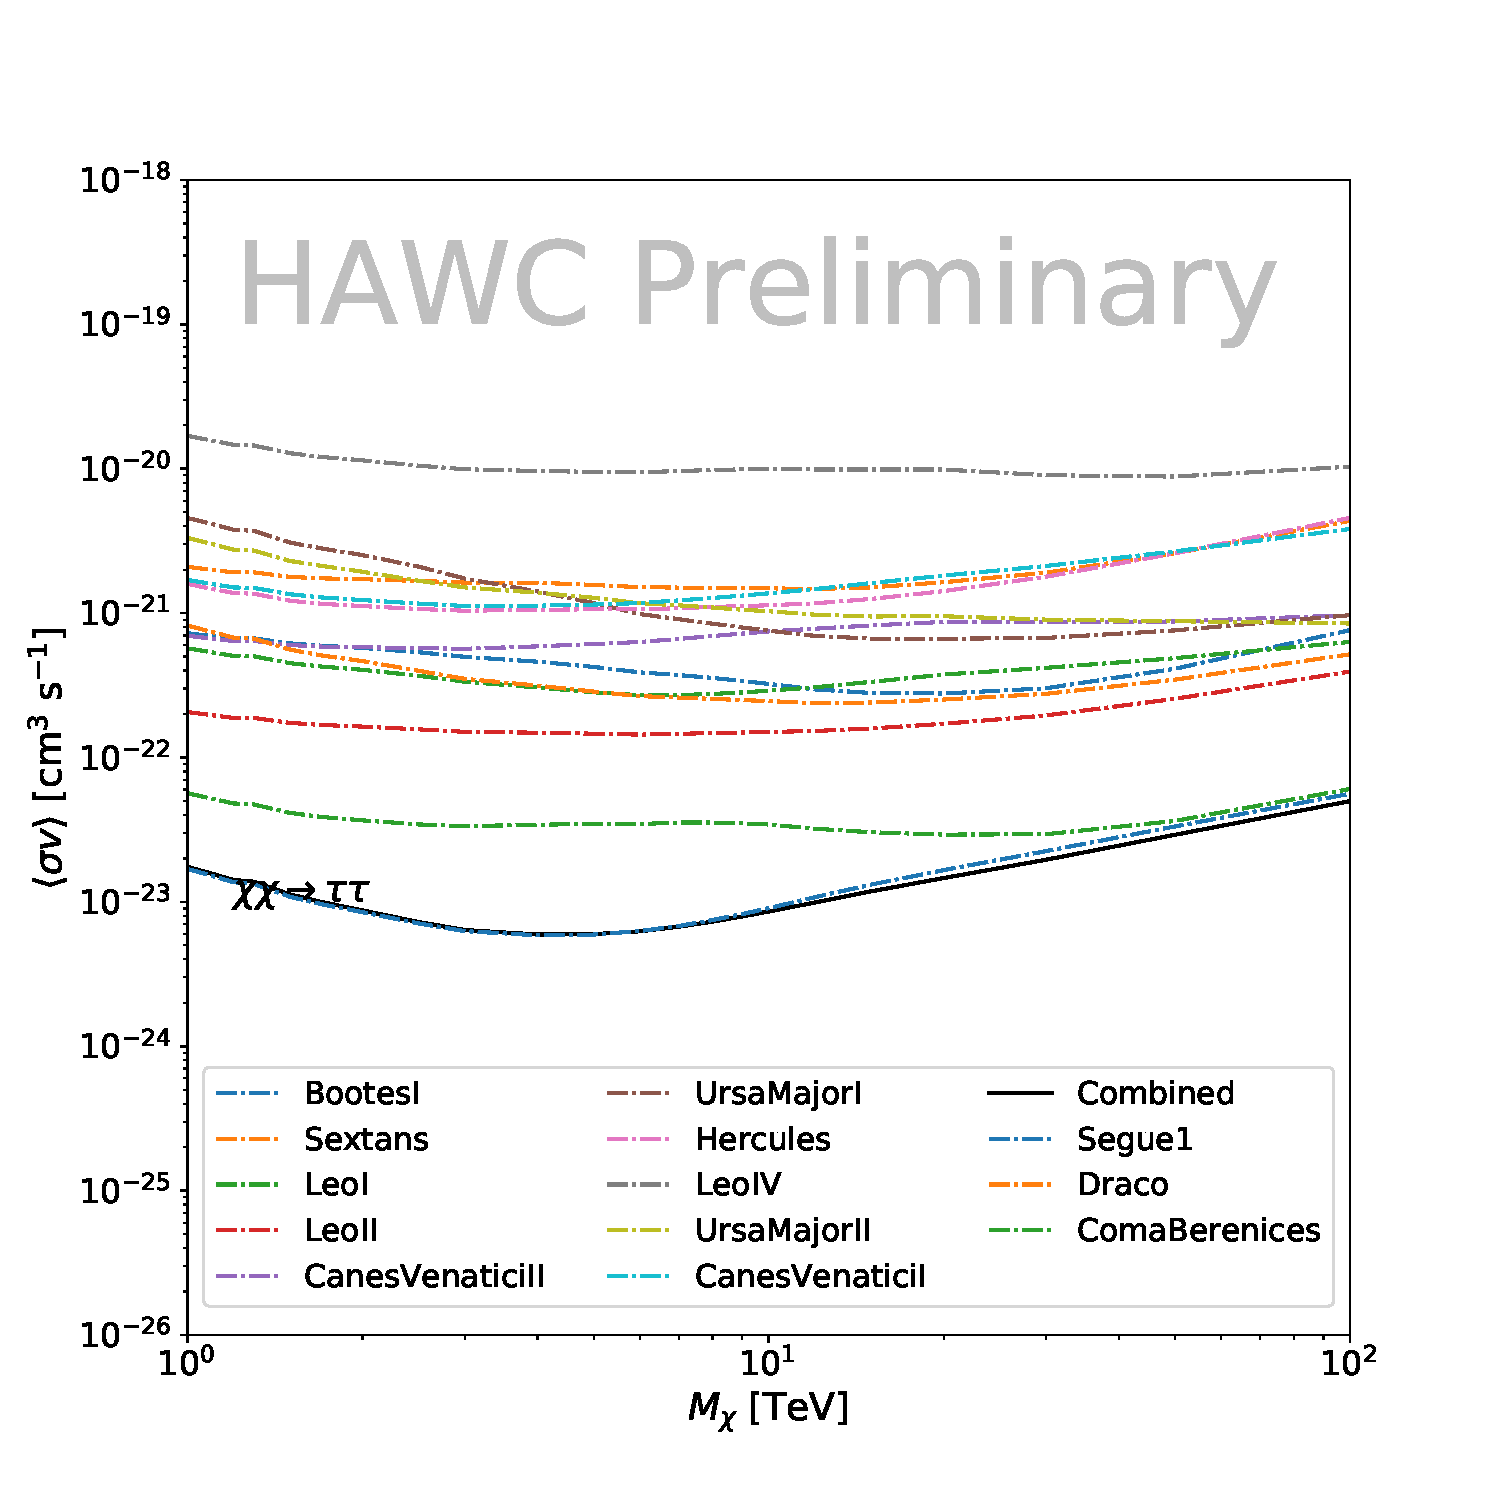
\includegraphics[scale=0.21]{figures/glory_duck/hawc/Combined95_GD_tautau.pdf}
    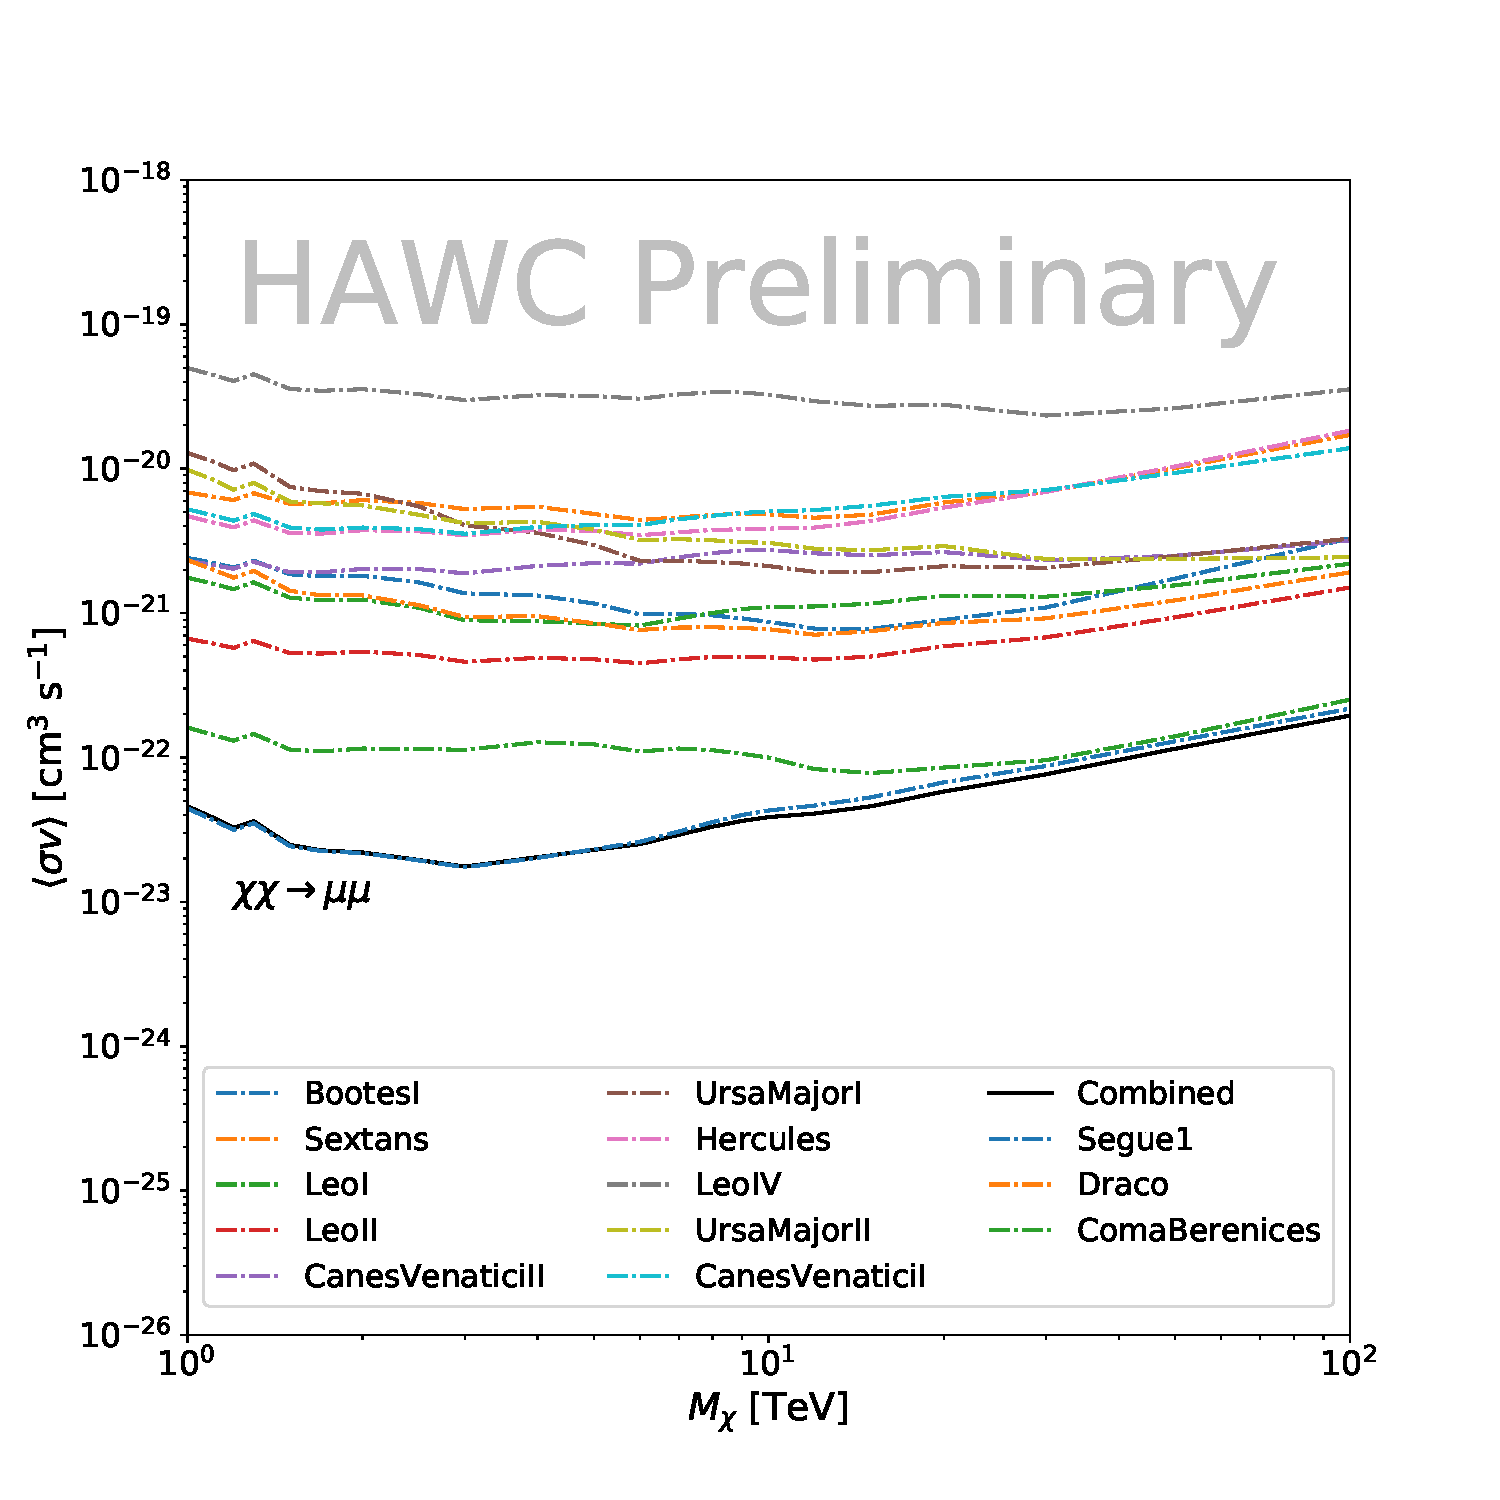
\includegraphics[scale=0.21]{figures/glory_duck/hawc/Combined95_GD_mumu.pdf}
    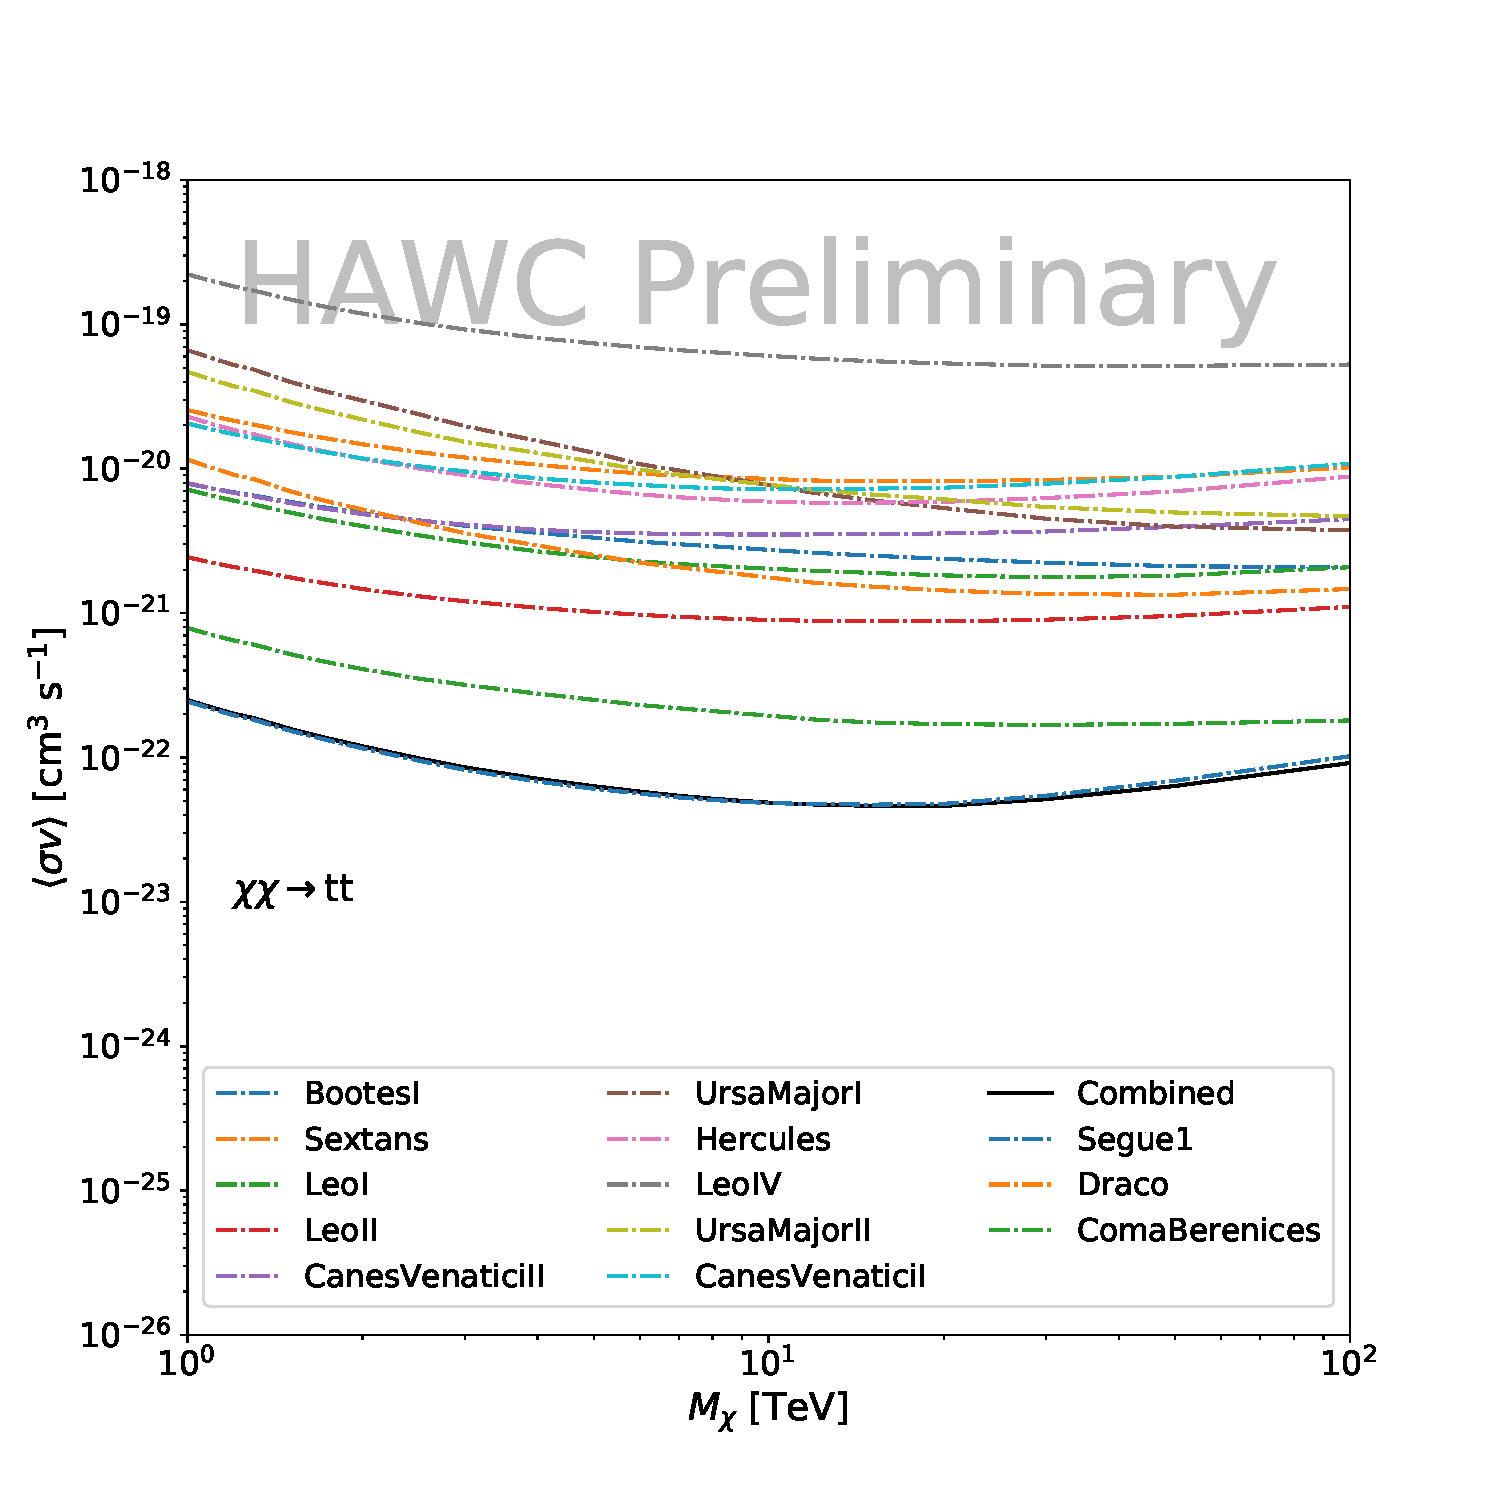
\includegraphics[scale=0.21]{figures/glory_duck/hawc/Combined95_GD_tt.pdf}
    }
    \caption{HAWC upper limits at 95\% confidence level on \sv versus DM mass for seven annihilation channels, using the set of \J-factors from Ref. \cite{Geringer-Sameth:2014yza} The solid line represents the observed combined limit. Dashed lines represent limits from individual dSphs.}
 \label{fig:hawc_combined_limit}
\end{figure}

% %\newpage
\begin{figure}[ht]
    \centering{\includegraphics[scale=0.21]{figures/glory_duck/hawc/GD_BrazilBand_bb.pdf}
    \includegraphics[scale=0.21]{figures/glory_duck/hawc/GD_BrazilBand_ee.pdf}
    \includegraphics[scale=0.21]{figures/glory_duck/hawc/GD_BrazilBand_mumu.pdf}
    \includegraphics[scale=0.21]{figures/glory_duck/hawc/GD_BrazilBand_tautau.pdf}
    \includegraphics[scale=0.21]{figures/glory_duck/hawc/GD_BrazilBand_ww.pdf}
    \includegraphics[scale=0.21]{figures/glory_duck/hawc/GD_BrazilBand_zz.pdf}
    \includegraphics[scale=0.21]{figures/glory_duck/hawc/GD_BrazilBand_tt.pdf}
    }
    \caption{HAWC Brazil bands at 95\% confidence level on \sv versus DM mass for seven annihilation channels with \J-factors from \GS \cite{Geringer-Sameth:2014yza}. The solid line represents the combined limit from 13 dSphs. The dashed line is the expected limit. The green band is the 68\% containment. The yellow band is the 95\% containment.}
\label{fig:hawc_brazil_band}
\end{figure}

%%%%%%%%%%%%%%%%%%%%%%%%%%%%%%%%%%%%%%%%%%%%%%%%%%%%%%%
\section{Glory Duck Combined Results}\label{sec:results}
%%%%%%%%%%%%%%%%%%%%%%%%%%%%%%%%%%%%%%%%%%%%%%%%%%%%%%%

The crux of this analysis is that HAWC's results are combined with 4 other gamma-ray observatories: Fermi-LAT, H.E.S.S., MAGIC, and VERITAS.
The complete joint likelihood for the \emph{l}-th dSph is the product of likelihood functions of the 5 experiments.

\todo{place holder for results}

No significant DM emission was observed by any of the five telescopes.
We present upper limits on \sv using the test statistics, \cref{eq:gd_TS}.

\begin{equation}
    \mathrm{TS} = -2 \ln{ \lambda(\svtex)},
\end{equation}

\sloppy No significant DM emission was observed by any of the five instruments.
We present the upper limits on \sv assuming seven independent DM self annihilation channels, namely $W^+W^-$, $Z^+Z^-$, $b\bar{b}$, $t\bar{t}$, $e^+e^-$, $\mu^+\mu^-$, and $\tau^+\tau^-$.
The 68\% and 95\% containment bands are produced from 300 Poisson realizations of the null hypothesis corresponding to each of the combined datasets.
These 300 realizations are combined identically to dSph observations.
The containment bands and the median are extracted from the distribution of resulting limits on the null hypothesis.
These 300 realizations are obtained either by fast simulations of the OFF observations, for H.E.S.S., MAGIC, VERITAS, and HAWC, or taken from real observations of empty fields of view in the case of Fermi-LAT~\cite{2015PhRvL.115w1301A,Fermi-LAT:2016uux,2021PhRvD.103l3005D}.

The obtained limits are shown in \Cref{fig:limits-geringer-sameth} for the \GS set of \J-factors~\cite{Geringer-Sameth:2014yza} and in \Cref{fig:limits-bonnivard} for the \B set of \J-factors~\cite{Bonnivard:2014kza, Bonnivard:2015xpq}.
The combined limits are presented with their 68\% and 95\% containment bands, and are expected to be close to the median limit when no signal is present.
We observe agreement with the null hypothesis for all channels, within $2\sigma$ standard deviations, between the observed limits and the expectations given by the median limits.
Limits obtained from each detector are also indicated in the figures, where limits for all dSphs observed by the specific instrument have been combined.

Below \textasciitilde300 GeV, the $Fermi$-LAT dominates the DM limits for all annihilation channels.
From \textasciitilde300 GeV to \textasciitilde2 TeV, $Fermi$-LAT continues to dominate for the hadronic and bosonic DM channels, yet the IACTs (H.E.S.S., MAGIC, and VERITAS) and $Fermi$-LAT all contribute to the limit for leptonic DM channels.
For DM masses between \textasciitilde2 TeV to \textasciitilde10 TeV, the IACTs dominate leptonic DM annihilation channels, whereas both the $Fermi$-LAT and the IACTs dominate bosonic and hadronic DM annihilation channels.
From \textasciitilde10 TeV to \textasciitilde100 TeV, both the IACTs and HAWC contribute significantly to the leptonic DM limit.
For hadronic and bosonic DM, the IACTs and $Fermi$-LAT both contribute strongly.

We notice that the limits computed using the \B set of \J-factor are always better compared to the ones calculated with the \GS set.
For the $W^+W^-$, $Z^+Z^-$, $b\bar{b}$, and $t\bar{t}$ channels, the ratio between the limits computed with the two sets of \J-factor is varying between a factor of \textasciitilde3 and \textasciitilde5 depending on the energy, with the largest ratio around 10~TeV.
For the channels $e^+e^-$, $\mu^+\mu^-$, and $\tau^+\tau^-$, the ratio lies between \textasciitilde2 to \textasciitilde6, being maximum around 1~TeV.
Examining \Cref{fig:comparison_J_1} and \Cref{fig:comparison_J_2} in \Cref{sec:gd_jfactor_systematic}, these differences are explained by the fact that the \B set provides higher \J-factors for the majority of the studied dSphs, with the notable exception of Segue~I.
The variation on the ratio of the limits for the two sets is due to different dSph dominating the limits depending on the energy.
This pushes the range of thermal cross-section which can be excluded to higher mass.
This comparison demonstrates the magnitude of systematic uncertainties associated with the choice of the \J-factor

This comparison demonstrates the magnitude of systematic uncertainties associated with the choice of the \J-factor calculation.
The \GS and \B sets present a difference in the limits for all channels of about
% (to be calculated by people having the numbers in hand)}.
This difference is explained, see  \Cref{fig:comparison_J_1} and \Cref{fig:comparison_J_2} in Appendix, by the fact that the \B set provides higher \J factors for all dSph except for Segue~I. This pushes the range of thermal cross-section which can be excluded to higher mass.

\begin{figure}[h!]
\centering{
\begin{tabular}{cc}
    \includegraphics[width=0.35\textwidth]{figures/glory_duck/limits/Glory_Duck_Annihilation_WW_Geringer-Sameth_Combination_bands.pdf} &
    \includegraphics[width=0.35\textwidth]{figures/glory_duck/limits/Glory_Duck_Annihilation_ZZ_Geringer-Sameth_Combination_bands.pdf} \\
    \includegraphics[width=0.35\textwidth]{figures/glory_duck/limits/Glory_Duck_Annihilation_bb_Geringer-Sameth_Combination_bands.pdf} &
    \includegraphics[width=0.35\textwidth]{figures/glory_duck/limits/Glory_Duck_Annihilation_tt_Geringer-Sameth_Combination_bands.pdf} \\
    \includegraphics[width=0.35\textwidth]{figures/glory_duck/limits/Glory_Duck_Annihilation_ee_Geringer-Sameth_Combination_bands.pdf} &
    \includegraphics[width=0.35\textwidth]{figures/glory_duck/limits/Glory_Duck_Annihilation_mumu_Geringer-Sameth_Combination_bands.pdf} \\
    \includegraphics[width=0.35\textwidth]{figures/glory_duck/limits/Glory_Duck_Annihilation_tautau_Geringer-Sameth_Combination_bands.pdf} &
    \end{tabular}
    }
    \caption{Upper limits at 95\% confidence level on \sv in function of the DM mass for eight annihilation channels, using the set of \J factors from Ref.~\cite{Geringer-Sameth:2014yza} (\GS set in \Cref{tab:gd_J_factor}). The black solid line represents the observed combined limit, the black dashed line is the median of the null hypothesis corresponding to the expected limit, while the green and yellow bands show the 68\% and 95\% containment bands. Combined upper limits for each individual detector are also indicated as solid, colored lines.
    %\jr{do not use light green for any line, since it gets confused with the 1sigma band}.
    The value of the thermal relic cross-section in function of the DM mass is given as the red dotted-dashed line~\cite{Bertone_2005}.}
\label{fig:limits-geringer-sameth}
\end{figure}


\begin{figure}[ht]
\centering{
\begin{tabular}{cc}
    \includegraphics[width=0.35\textwidth]{figures/glory_duck/limits/Glory_Duck_Annihilation_WW_Bonnivard_Combination_bands.pdf} &
    \includegraphics[width=0.35\textwidth]{figures/glory_duck/limits/Glory_Duck_Annihilation_ZZ_Bonnivard_Combination_bands.pdf} \\
    \includegraphics[width=0.35\textwidth]{figures/glory_duck/limits/Glory_Duck_Annihilation_bb_Bonnivard_Combination_bands.pdf} &
    \includegraphics[width=0.35\textwidth]{figures/glory_duck/limits/Glory_Duck_Annihilation_tt_Bonnivard_Combination_bands.pdf} \\
    \includegraphics[width=0.35\textwidth]{figures/glory_duck/limits/Glory_Duck_Annihilation_ee_Bonnivard_Combination_bands.pdf} &
    \includegraphics[width=0.35\textwidth]{figures/glory_duck/limits/Glory_Duck_Annihilation_mumu_Bonnivard_Combination_bands.pdf} \\
    \includegraphics[width=0.35\textwidth]{figures/glory_duck/limits/Glory_Duck_Annihilation_tautau_Bonnivard_Combination_bands.pdf} &
    \end{tabular}
    }
    \caption{Same as \cref{fig:limits-geringer-sameth}, using the set of \J factors from Ref.~\cite{Bonnivard:2014kza, Bonnivard:2015xpq} (\B set in \Cref{tab:gd_J_factor}).}
\label{fig:limits-bonnivard}
\end{figure}

\begin{figure}[ht]
\centering{
\begin{tabular}{ccc}
    \includegraphics[width=0.3\textwidth]{figures/glory_duck/comparison/GD_limits_WW.pdf} &
    \includegraphics[width=0.3\textwidth]{figures/glory_duck/comparison/GD_limits_ZZ.pdf} &
    \includegraphics[width=0.3\textwidth]{figures/glory_duck/comparison/GD_limits_bb.pdf} \\
    \includegraphics[width=0.3\textwidth]{figures/glory_duck/comparison/GD_limits_tt.pdf} &
    \includegraphics[width=0.3\textwidth]{figures/glory_duck/comparison/GD_limits_ee.pdf} &
    \includegraphics[width=0.3\textwidth]{figures/glory_duck/comparison/GD_limits_mumu.pdf} \\
    \includegraphics[width=0.3\textwidth]{figures/glory_duck/comparison/GD_limits_tautau.pdf} &
    \end{tabular}
    }
    \caption{Comparisons of the combined limits at 95\% confidence level for each of the eight annihilation channels when using the \J factors from Ref.~\cite{Geringer-Sameth:2014yza} (\GS set in \Cref{tab:gd_J_factor}), plain lines, and the \J factor from Ref.~\cite{Bonnivard:2014kza, Bonnivard:2015xpq} (\B set in \Cref{tab:gd_J_factor}), dashed lines. The cross-section given by the thermal relic is also indicated~\cite{Bertone_2005}.}
\label{fig:limits-comparison}
\end{figure}

%%%%%%%%%%%%%%%%%%%%%%%%%%%%%%%%%%%%%%%%%%%%%%%%%%%%%%%%%%%%%%%%%%%%%%%%%%%%%%%%%%%%%
\section{HAWC Systematics} \label{sec:hawc_systematic}
%%%%%%%%%%%%%%%%%%%%%%%%%%%%%%%%%%%%%%%%%%%%%%%%%%%%%%%%%%%%%%%%%%%%%%%%%%%%%%%%%%%%%

%%%%%%%%%%%%%%%%%%%%%%%%%%%%%%%%%%%%%%%%%%%%%%%%%%%%%%%%%%%%%%%%%%%%
\subsection{Inverse Compton Scattering} \label{sec:gd_ics}
%%%%%%%%%%%%%%%%%%%%%%%%%%%%%%%%%%%%%%%%%%%%%%%%%%%%%%%%%%%%%%%%%%%%
The DM-DM annihilation channels produce many high energy electrons regardless of the primary annihilation channel.
These high energy electrons can produce high energy gamma-rays through Inverse Compton Scattering (ICS).
If this effect is strong, it would change the morphology of the source and increase the total expected gamma-ray counts from any source.
The PPPC \cite{Cirelli_2011} provides tools in Mathematica for calculating the impact of ICS for an arbitrary location in the sky for a specified annihilation channel.
We calculated the change in gamma-ray counts for DM annihilation to primary $e\bar{e}$ for RA and Dec corresponding to Segue1 and Coma Berenices.
These dSphs were chosen because they are the strongest contributors to the limit.
$e\bar{e}$ was selected because it would have the largest number of high energy electrons.
The effect was found to be on the order of $~10^{-7}$ on the gamma-ray spectrum.
As a result, this systematic is not considered in our analysis.

%%%%%%%%%%%%%%%%%%%%%%%%%%%%%%%%%%%%%%%%%%%%%%%%%%%%%%%%%%%%%%%%%%%%
\subsection{Point Source Versus Extended Source Limits}\label{sec:gd_ext_limitvs_ptsrc}
%%%%%%%%%%%%%%%%%%%%%%%%%%%%%%%%%%%%%%%%%%%%%%%%%%%%%%%%%%%%%%%%%%%%

The previous DM search toward dSph approximated the dSphs as point sources \cite{Albert_2018}.
In this analysis, the dSphs are implemented as extended with J-factor distributions following those produced by \cite{Geringer-Sameth:2014yza}.
The resolution of the cited map is much finer than HAWC's angular resolution.
The vast majority of the J-factor distribution is represented on the central HAWC pixel of the dSph spatial map.
However, the neighboring 8 pixels are not negligible and contribute to our limit.

\begin{figure}[ht]
\centering{
    \includegraphics[scale=0.19]{figures/glory_duck/hawc/95Lim_Segue1_ExtVsPt.pdf}}
    \caption{Comparisons of the combined limits at 95\% confidence level for a point source analysis and extended source using ~\cite{Geringer-Sameth:2014yza} \GS J-factor distributions and PPPC \cite{Cirelli_2011} annihilation spectra. Shown are the limits for Segue1 which will have the most significant impact on the combined limit. 6 of the 7 DM annihilation channels are shown. Solid lines are extended source studies. Dashed lines are point source studies. Overall, the extended source analysis improves the limit by a factor of 2.}
\label{fig:Seg1point_versus_extended}
\end{figure}

\begin{figure}[h]
\centering{
    \includegraphics[scale=0.19]{figures/glory_duck/hawc/95Lim_ComaBerenices_ExtVsPt.pdf}}
    \caption{Same as \cref{fig:Seg1point_versus_extended} on Coma Berenices. This dSph also contributes significantly to the limit. The limits are identical in this case.}
\label{fig:ComaBpoint_versus_extended}
\end{figure}

\Cref{fig:Seg1point_versus_extended} shows a substantial improvement to the limit for Segue1.
\cref{fig:ComaBpoint_versus_extended} however showed identical limits.
These disparities are best explained by the relative difference in their J-Factors.
Both dSphs pass almost overhead the HAWC detector, however Segue1 has the larger J-Factor between the two.
Adjacent pixels to the central pixel will therefor contribute to the limits.
This is the case for other dSph that are closer to overhead the HAWC detector.

Comparison plots for all sources and the combined limit can be found in the sandbox for the Glory Duck project.

%%%%%%%%%%%%%%%%%%%%%%%%%%%%%%%%%%%%%%%%%%%%%%%%%%%%%%%%%%%%%%%%%%%%
\subsection{Impact of Pointing Systematic}\label{sec:gd_pointing_sys}
%%%%%%%%%%%%%%%%%%%%%%%%%%%%%%%%%%%%%%%%%%%%%%%%%%%%%%%%%%%%%%%%%%%%

During the analysis it was discovered that reconstruction of gamma-rays.
Slides describing this systematic can be found \href{https://private.hawc-observatory.org/wiki/images/3/30/HAWCMeetingOct2020-AJS-Pointing.pdf}{here}.
Shown on the presentation is dependence on the pointing systematic on declination.
New spatial profiles were generated for every dSph and limits were computed for the adjusted declination.

\Cref{fig:pointing_systematic} demonstrates the impact of this systematic for all DM annihilation channels studied by HAWC. The impact is a tiny improvement, yet mostly identical, to the combined limits.

\begin{figure}[h]
\centering{
    \includegraphics[scale=0.21]{figures/glory_duck/hawc/PointingSystematic_GD_Combined_bb.pdf}
    \includegraphics[scale=0.21]{figures/glory_duck/hawc/PointingSystematic_GD_Combined_ee.pdf}
    \includegraphics[scale=0.21]{figures/glory_duck/hawc/PointingSystematic_GD_Combined_mumu.pdf}
    \includegraphics[scale=0.21]{figures/glory_duck/hawc/PointingSystematic_GD_Combined_tautau.pdf}
    \includegraphics[scale=0.21]{figures/glory_duck/hawc/PointingSystematic_GD_Combined_tt.pdf}
    \includegraphics[scale=0.21]{figures/glory_duck/hawc/PointingSystematic_GD_Combined_ww.pdf}
    \includegraphics[scale=0.21]{figures/glory_duck/hawc/PointingSystematic_GD_Combined_zz.pdf}
    \caption{Comparison of combined limits when correcting for HAWC's pointing systematic. All DM annihilation channels are shown. The solid black line is the ratio between published limit to the declination corrected limit. The blue solid line or "Combined\_og" represented the limits computed for Glory Duck. The solid orange line or "Combined\_ad" represented the limits computed after correcting for the pointing systematic.}
}
\label{fig:pointing_systematic}
\end{figure}

%%%%%%%%%%%%%%%%%%%%%%%%%%%%%%%%%%%%%%%%%%%%%%%%%%%%%%%%%
\section{\J-factor distributions}\label{sec:gd_jfactor_systematic}
%%%%%%%%%%%%%%%%%%%%%%%%%%%%%%%%%%%%%%%%%%%%%%%%%%%%%%%%%

%%%%%%%%%%%%%%%%%%%%%%%%%%%%%%%%%%%%%%%%%%%%%%%%%%%%%%%%%
\subsection{Numerical integration of \GS maps}\label{sec:gd_jfacintegration}
%%%%%%%%%%%%%%%%%%%%%%%%%%%%%%%%%%%%%%%%%%%%%%%%%%%%%%%%%

It was discovered well after the HAWC anaylsis was completed that the published tables from \GS \cite{Geringer_Sameth_2015} quoted median \J-factors were computed in a non-trivial manner.
The assumption myself and collaborators had was that the published tables represented the \J-factor as a function of $\theta$ for the best global fit model on a per source basis.
However, this is not the case.
Instead, what is published are the best fit model for each dwarf that only considers stars up to the angular separation $\theta$.
Therefore, the model is changing for each value of $\theta$ for each dwarf.

Median \J-factor model profiles were provided by the authors.
New maps were generated and analyzed for Segue1 and Coma Berenices.
\tmpfig{Differential maps}

Upper limits were again calculated for the two sources for each DM annihilation channel.
\tmpfig{New limits with different maps}

%%%%%%%%%%%%%%%%%%%%%%%%%%%%%%%%%%%%%%%%%%%%%%%%%%%%%%%%%
\subsection{\GS versus \B spatial models}\label{sec:gd_gsVb}
%%%%%%%%%%%%%%%%%%%%%%%%%%%%%%%%%%%%%%%%%%%%%%%%%%%%%%%%%

We show in this appendix a comparison between the \J-factors computed by Geringer-Sameth \emph{et al.}~\cite{Geringer-Sameth:2014yza} (the \GS set) and the ones computed by Bonnivard \emph{et al.}~\cite{Bonnivard:2014kza, Bonnivard:2015xpq} (the \B set).
%The differences in computation between both sets are detailed in \cref{sec:DM}.
%
The \GS \J-factors are computed through a Jeans analysis of the kinematic stellar data of the  selected dSphs, assuming a dynamic equilibrium and a spherical symmetry for the dSphs.
They adopted the generalized DM density distribution, known as Zhao-Hernquist, introduced by~\cite{Zhao:1995cp}, carrying three additional index parameters to describe the inner and outer slopes, and the break of the density profile.
Such a profile parametrization allows the reduction of the theoretical bias from the choice of a specific radial dependency on the kinematic data.
In other words, the increase of free parameters with the use of the  Zhao-Hernquist profile allows a better description of the mass density distribution of dark matter.

In addition, a constant velocity anisotropy profile and a Plummer light profile \cite{10.1093/mnras/71.5.460} for the stellar distribution were assumed.
The velocity anisotropy profile depends on the radial and tangential velocity dispersions.
However, its determination remains challenging since only the line-of-sight velocity dispersion can be derived from velocity measurements.
Therefore, the parametrization of the anisotropy profile is obtained from simulated halos (see~\cite{Hunter:2013vua} for more details).
They provide the values of the \J-factors of regions extending to various angular radius up to the outermost member star.

% using a uniform analysis of the most recent stellar-kinematic data available
% %generalized density profile
% %Assuming dynamic equilibrium and spherical symmetry, these quantities are related according to the spherical Jeans
% %\cite{Geringer-Sameth:2014yza}

% %We also use the set of  \B \J-factors in order to obtain an estimate of the systematic uncertainty  on the $\sv$ upper limits from the assumed \J-factor value.
The \B \J-factors were computed through a Jeans analysis taking into account the systematic uncertainties induced by the DM profile parametrization, the radial velocity anisotropy profile, and the triaxiality of the halo of the dwarf galaxies.
They performed a more complete study of the dSph kinematics and dynamics than \GS for the determination of the \J-factor.
Conservative values of the \J-factors where obtained using an Einasto DM density profile~\cite{Dhar_2010}, a realistic anisotropy profile known as the Baes \& Van Hese profile~\cite{Baes:2007tx} which takes into account that the inner regions can be significantly non-isotropic, and a Zhao-Hernquist light profile~\cite{Zhao:1995cp}.

For both sets, \J-factor values are provided for all dSphs as a function of the radius of the integration region~\cite{Geringer-Sameth:2014yza,Bonnivard:2014kza,Bonnivard:2015xpq}.
\Cref{tab:gd_J_factor} shows the heliocentric distance and Galactic coordinates of the twenty dSphs, together with the two sets of \J-factor values integrated up to the outermost observed star for \GS and the tidal radius for \B.
Both \J-factor sets were derived through a Jeans analysis based on the same kinematic data, except for Draco where the measurements of~\cite{2015MNRAS.448.2717W} have been adopted in the computation of the \B value.
The computations for producing the \GS and \B samples differ in the choice of the DM density, velocity anisotropy, and light profiles, for which the set \B takes into account some sources of systematic uncertainties.

\Cref{fig:comparison_J_1} and \Cref{fig:comparison_J_2} show the comparisons for the \J-factor versus the angular radius for each of the 20 dSphs used in this study.
The uncertainties provided by the authors are also indicated in the figures.
For the \GS set, the computation stops at the angular radius corresponding to the outermost observed star, while for the \B set, the computation stops at the angular radius corresponding to the tidal radius.

\begin{figure}[ht]
\centering{
    \includegraphics[scale=0.32]{figures/glory_duck/appendix/BootesI.pdf}
    \includegraphics[scale=0.32]{figures/glory_duck/appendix/CanesVenaticiI.pdf}
    \includegraphics[scale=0.32]{figures/glory_duck/appendix/CanesVenaticiII.pdf}
    \includegraphics[scale=0.32]{figures/glory_duck/appendix/Carina.pdf}
    \includegraphics[scale=0.32]{figures/glory_duck/appendix/ComaBerenices.pdf}
    \includegraphics[scale=0.32]{figures/glory_duck/appendix/Draco.pdf}
    \includegraphics[scale=0.32]{figures/glory_duck/appendix/Fornax.pdf}
    \includegraphics[scale=0.32]{figures/glory_duck/appendix/Hercules.pdf}
    \includegraphics[scale=0.32]{figures/glory_duck/appendix/LeoI.pdf}
    \includegraphics[scale=0.32]{figures/glory_duck/appendix/LeoII.pdf}
    }
    \caption{Comparisons between the \J-factors versus the angular radius for the computation of $J$ factors from Ref.~\cite{Geringer-Sameth:2014yza} (\GS set in \Cref{tab:gd_J_factor}) in blue and for the computation from Ref.~\cite{Bonnivard:2014kza, Bonnivard:2015xpq} (\B set in \cref{tab:gd_J_factor}) in orange. The solid lines represent the central value of the \J-factors while the shaded regions correspond to the 1$\sigma$ standard deviation.}
\label{fig:comparison_J_1}
\end{figure}

\begin{figure}[ht]
\centering{
    \includegraphics[scale=0.32]{figures/glory_duck/appendix/LeoIV.pdf}
    \includegraphics[scale=0.32]{figures/glory_duck/appendix/LeoT.pdf}
    \includegraphics[scale=0.32]{figures/glory_duck/appendix/LeoV.pdf}
    \includegraphics[scale=0.32]{figures/glory_duck/appendix/Sculptor.pdf}
    \includegraphics[scale=0.32]{figures/glory_duck/appendix/SegueI.pdf}
    \includegraphics[scale=0.32]{figures/glory_duck/appendix/SegueII.pdf}
    \includegraphics[scale=0.32]{figures/glory_duck/appendix/Sextans.pdf}
    \includegraphics[scale=0.32]{figures/glory_duck/appendix/UrsaMajorI.pdf}
    \includegraphics[scale=0.32]{figures/glory_duck/appendix/UrsaMajorII.pdf}
    \includegraphics[scale=0.32]{figures/glory_duck/appendix/UrsaMinor.pdf}
}
    \caption{Comparisons between the \J-factors versus the angular radius for the computation of $J$ factors from Ref.~\cite{Geringer-Sameth:2014yza} (\GS set in \cref{tab:gd_J_factor}) in blue and for the computation from Ref.~\cite{Bonnivard:2014kza, Bonnivard:2015xpq} (\B set in \cref{tab:gd_J_factor}) in orange. The solid lines represent the central value of the \J-factors while the shaded regions correspond to the 1$\sigma$ standard deviation.}
\label{fig:comparison_J_2}
\end{figure}

%%%%%%%%%%%%%%%%%%%%%%%%%%%%%%%%%%%%%%%%%%%%%%%%%%%%%%%%%
\section{Discussion and Conclusions\label{sec:gd_conclusions}}
%%%%%%%%%%%%%%%%%%%%%%%%%%%%%%%%%%%%%%%%%%%%%%%%%%%%%%%%%

In this multi-instrument analysis, we have used observations of 20 dSphs from the gamma-ray telescopes Fermi-LAT, H.E.S.S., MAGIC, VERITAS, and HAWC to perform a collective DM search annihilation signals.
The data were combined across sources and detectors to significantly increase the sensitivity of the search.
We have observed no significant deviation from the null, no DM, hypothesis, and so present our results in terms of upper limits on the annihilation cross section for seven potential DM annihilation channels.

Fermi-LAT brings the most stringent constraints for continuum channels below approximately 1~TeV. the remaining detectors dominate at higher energies.
Overall, for multi-TeV DM mass, the combined DM constraints from all five telescopes are 2-3 times stronger than any individual telescope for multi-TeV DM.

Derived from observations of many dSphs, our results produce robust limits given the DM content of the dSphs is relatively well constrained.
The obtained limits span the largest mass range of any WIMP DM search.
Our combined analysis improves the sensitivity over previously published results from each detectors which produces the most stringent limits on DM annihilation from dSphs.
These results are based on deep exposures of the most promising known dSphs with the currently most sensitive gamma-ray instruments.
Therefore, our results constitute a legacy of a generation of gamma-ray instruments on WIMP DM searches towards dSphs.
Our results will remain the reference in the field until a new generation of more sensitive gamma-ray instruments begin operations, or until new dSphs with higher \J-factors are discovered.

This analysis serves as a proof of concept for future multi-instrument and multi-messenger combination analyses.
With this collaborative effort, we have managed to sample over four orders in magnitude in gamma-ray energies with distinct observational techniques.
Determining the nature of DM continues to be an elusive and difficult problem.
Larger datasets with diverse measurement techniques could be essential to tackling the DM problem.
A future collaboration using similar techniques as the ones described in this paper could grow even beyond gamma rays.
The models we used for this study include annihilation channels with neutrinos in the final state.
Advanced studies could aim to merge our results with those from neutrino observatories with large data sets.
Efforts are already underway to add data from the IceCube, ANTARES, and KM3NeT observatories to these gamma-ray results.

From this work, a selection of the best candidates for observations, according to the latest knowledge on stellar dynamics and modelling techniques for the derivation of the \J-factors on the potential dSphs targets, is highly desirable at the time that new experiments are starting their dark matter programmes using dSphs.
Given the systematic uncertainty inherent to the derivation of the \J-factors,
an informed observational strategy would be to select both objects with the highest \J-factors that could lead to DM signal detection, and objects with robust \J-factor predictions, i.e. with kinematic measurements on many bright stars, which would strengthen the DM interpretation reliability of the observation outcome.

This analysis combines data from multiple telescopes to produce strong constraints on astrophysical objects.
From this perspective, these methods can be applied beyond just DM searches.
Almost every astrophysical study can benefit from multi-telescope, multi-wavelength gamma-ray studies.
We have enabled these telescopes to study the cosmos with greater precision and detail.
Many astrophysical searches can benefit from multi-instrument gamma-ray studies, for which our analysis lays the foundation.

%%%%%%%%%%%%%%%%%%%%%%%%%%%%%%%%%%%%%%%%%%%%%%%%%%%%%%%%%%%%%%%%%%%%%%%%%%%%%%%%%%%%%
\chapter{Multithreading HAWC analyses for Dark Matter Searches} \label{sec:multithread}
%%%%%%%%%%%%%%%%%%%%%%%%%%%%%%%%%%%%%%%%%%%%%%%%%%%%%%%%%%%%%%%%%%%%%%%%%%%%%%%%%%%%%
%%%%%%%%%%%%%%%%%%%%%%%%%%%%%%%%%%%%%%%%%%%%%%%%%%%%%%%%%%%%%%%%%%%%%%%%%%%%%%%%%%%%%
\section{Introduction}\label{sec:mtd_intro}
%%%%%%%%%%%%%%%%%%%%%%%%%%%%%%%%%%%%%%%%%%%%%%%%%%%%%%%%%%%%%%%%%%%%%%%%%%%%%%%%%%%%%

HAWC's current software suite, plugins to 3ML, does not fully utilize computational advancements of recent decades.
Said advancements include the proliferation of Graphical Processing Units (GPUs), and multithreading on multi-core processors.
The analysis described in \Cref{sec:glory_duck} took up to 3 months of human time waiting for the full gambit of data analysis and simulation of background to run.
Additionaly, with the addition of a 2D binning scheme, $f_\mathrm{hit}$ and NN, the compute time is expected to grow.
Although excessive computing time was, in part, from an intense use of a shared computing cluster, it was evident that there was room for improvement.
In HAWC's next generation dSph DM search, I decided to develop codes that would utilize the multi-core processors on modern high performance computing clusters.
The results of this work are featured in this chapter and brought a human timing improvement to computation that scales as $1/N$ where $N$ is the number of threads.

%%%%%%%%%%%%%%%%%%%%%%%%%%%%%%%%%%%%%%%%%%%%%%%%%%%%%%%%%%%%%%%%%%%%%%%%%%%%%%%%%%%%%
\section{Dataset and Background}\label{sec:mtd_databgd}
%%%%%%%%%%%%%%%%%%%%%%%%%%%%%%%%%%%%%%%%%%%%%%%%%%%%%%%%%%%%%%%%%%%%%%%%%%%%%%%%%%%%%

This section enumerates the data and background methods used for HAWC's multi-threaded study of dSphs.
\Cref{sec:mtd_data} and \Cref{sec:mtd_tools} are most useful for fellow HAWC collaborators looking to replicate a multithreaded dSph DM search.

%%%%%%%%%%%%%%%%%%%%%%%%%%%%%%%%%%%%%%%%%%%%%%%
\subsection{Itemized HAWC files}\label{sec:mtd_data}
%%%%%%%%%%%%%%%%%%%%%%%%%%%%%%%%%%%%%%%%%%%%%%%

\begin{itemize}
    \item Detector Resolution: \texttt{refit-Pass5-Final-NN-detRes-zenith-dependent.root}
    \item Data Map: \texttt{Pass5-Final-NN-maptree-ch103-ch1349-zenith-dependent.root}
    \item Spectral Dictionary: \texttt{HDMSpectra\_dict\_gamma.npy}
\end{itemize}

% %%%%%%%%%%%%%%%%%%%%%%%%%%%%%%%%%%%%%%%%%%%%%%%
\subsection{Software Tools and Development}\label{sec:mtd_tools}
%%%%%%%%%%%%%%%%%%%%%%%%%%%%%%%%%%%%%%%%%%%%%%%

This analysis was performed using HAL and 3ML \cite{Abeysekara_2017, vianello2015multimission} in Python version 3.
I built software in collaboration with Michael Martin and Letrell Harris to implement the \emph{Dark Matter Spectra from the Electroweak to the Planck Scale} (HDM) \cite{HDMSpectra} and dSphs spatial model from \cite{DM_Strigari20} for HAWC analysis.
A NumPy dictionary of HDM was made for Py3.
The corresponding Python3 file is \texttt{HDMSpectra\_dict\_gamma.npy}.
These files can also be used for decay channels and tools are provided in HDM's \href{https://github.com/nickrodd/HDMSpectra/tree/master}{git repository} \cite{HDMSpectra}.
The analysis was performed using the Neural Network energy estimator for Pass 5.F.
A description of this estimator was provided in \Cref{sec:hawc}.\todo{define a subsection when it's written}, and its key improvements are an improved energy estimation and improved sensitivities at higher zenith angles.
All other software used for data analysis, DM profile generation, and job submission to SLURM are also kept in my sandbox in the \href{https://gitlab.com/hawc-observatory/sandboxes/salaza82/dark_matter_hawc}{Dark Matter HAWC} project.
The above repository also incorporates the model inputs used previously in Glory Duck, described in \Cref{sec:glory_duck}

%%%%%%%%%%%%%%%%%%%%%%%%%%%%%%%%%%%%%%%%%%%%%%%
\subsection{Data Set and Background Description} \label{sec:mtd_data_bkgd}
%%%%%%%%%%%%%%%%%%%%%%%%%%%%%%%%%%%%%%%%%%%%%%%

The HAWC data maps used for this analysis contain 2565 days of data between runs 2104 (\todo{Day start}) and 7476 (\todo{day end}).
They were generated from pass 5.f reconstruction.
The analysis is performed using the NN energy estimator with bin list:

\begin{itemize}
    \item[] \texttt{B1C0Ea}, \texttt{B1C0Eb}, \texttt{B1C0Ec}, \texttt{B1C0Ed}, \texttt{B1C0Ee}, \texttt{B2C0Ea}, \texttt{B2C0Eb}, \texttt{B2C0Ec}, \texttt{B2C0Ed}, \texttt{B2C0Ee}, \texttt{B3C0Ea}, \texttt{B3C0Eb}, \texttt{B3C0Ec}, \texttt{B3C0Ed}, \texttt{B3C0Ee}, \texttt{B3C0Ef}, \texttt{B4C0Eb}, \texttt{B4C0Ec}, \texttt{B4C0Ed}, \texttt{B4C0Ee}, \texttt{B4C0Ef}, \texttt{B5C0Ec}, \texttt{B5C0Ed}, \texttt{B5C0Ee}, \texttt{B5C0Ef}, \texttt{B5C0Eg}, \texttt{B6C0Ed}, \texttt{B6C0Ee}, \texttt{B6C0Ef}, \texttt{B6C0Eg}, \texttt{B6C0Eh}, \texttt{B7C0Ee}, \texttt{B7C0Ef}, \texttt{B7C0Eg}, \texttt{B7C0Eh}, \texttt{B7C0Ei}, \texttt{B8C0Ee}, \texttt{B8C0Ef}, \texttt{B8C0Eg}, \texttt{B8C0Eh}, \texttt{B8C0Ei}, \texttt{B8C0Ej}, \texttt{B9C0Ef}, \texttt{B9C0Eg}, \texttt{B9C0Eh}, \texttt{B9C0Ei}, \texttt{B9C0Ej}, \texttt{B10C0Eg}, \texttt{B10C0Eh}, \texttt{B10C0Ei}, \texttt{B10C0Ej}, \texttt{B10C0Ek}, \texttt{B10C0El}
\end{itemize}
Bin 0 was excluded as it has substantial hadronic contamination and poor angular resolution.

Background considerations and source selection was identical to \Cref{sec:gd_databgd}, and no additional arguements are provided here.
Many of the HAWC systematics explored in \Cref{sec:hawc_systematic} also apply for this DM search and are not added upon here.

%%%%%%%%%%%%%%%%%%%%%%%%%%%%%%%%%%%%%%%%%%%%%%%%%%%%%%%%%%%%%%%%%%%%%%%%%%%%%%%%%%%%%
\section{Analysis}\label{sec:mtd_analysis}
%%%%%%%%%%%%%%%%%%%%%%%%%%%%%%%%%%%%%%%%%%%%%%%%%%%%%%%%%%%%%%%%%%%%%%%%%%%%%%%%%%%%%

The analysis and its systematics are almost identical to \Cref{sec:gd_analysis}.
Importantly, we use the same \Cref{eq:id_dm_flux} and \Cref{eq:jfactor} for estimating the gamma-ray flux at HAWC from our sources.
We add on to the previous study with a search for DM decay.
The flux equations for DM decay are
\iddmdecay[\gamma]

with a new quantity, the \D factor, defined as
\dfactor
Software was written to accomodate DM decay from dSphs, however decay profiles were not received from \LS by the time of writing this tehsis.

%%%%%%%%%%%%%%%%%%%%%%%%%%%%%%%%%%%%%%%%%%%%%%%%%%
\subsection{$\frac{dN_\gamma}{dE_\gamma}$ - Particle Physics Component}\label{sec:mtd_particlephysics}
%%%%%%%%%%%%%%%%%%%%%%%%%%%%%%%%%%%%%%%%%%%%%%%%%%

For these spectra, we import HDM with Electroweak (EW) corrections and additional corrections for neutrinos above the EW scale \cite{HDMSpectra}.
The spectrum is implemented as a model script in astromodels for 3ML.
A comprehensive description of EW corrections and neutrino considerations are provided later in \todo{refeance MM nu duck}.

\begin{figure}[t]
    \centering{
        \includegraphics[scale=0.8]{figures/mtd_hawc_dm/pppc_vs_hdm.png}
    }
    \caption{Difference between spectral hypotheses from PPPC \cite{Cirelli_2011} and HDM \cite{HDMSpectra}. Shown is the expected DM annihilation spectrum for $\chi\chi \rightarrow W^-W^+$. Solid lines are spectral models with EW corrections from the PPPC. Dash-dot lines are spectral models from HDM. Red lines are models for $M_\chi = 1$ TeV. Blue lines represent models for $M_\chi = 100$ TeV.}
    \label{fig:pppc_vs_hdm}
\end{figure}

\Cref{fig:pppc_vs_hdm} demonstrates the impact of changes from HDM on DM
annihilation to W bosons.
A class in astromodels was developed to include HDM and is aptly named \texttt{HDMSpectra} within \texttt{DM\_models.py}.
The SM DM annihilation channels studied here are $\chi\chi \rightarrow$:
\begin{itemize}
    \item[] $e^+e^-$, $\mu^+\mu^-$, $\tau^+\tau^-$,$b\bar{b}$, $t\bar{t}$, $gg$, $W^+W^-$, $ZZ$, $c\bar{c}$, $u\bar{u}$, $d\bar{d}$, $s\bar{s}$, $\nu_e \overline{\nu_e}$, $\nu_\mu \overline{\nu_\mu}$, $\nu_\tau \overline{\nu_\tau}$, $\gamma\gamma$, $hh$.
\end{itemize}
For $\gamma\gamma$ and $ZZ$, a substantial fraction of the signal photons are expected to have total energy equal $m_\chi$ \cite{HDMSpectra}.
This introduces a $\delta$-function that is much narrower than the energy resolution of the HAWC detector.
To ensure that this feature is not lost in the likelihood fits, the 'line' feature is convolved with a gausian kernel with a $1\sigma$ width of $0.05 \cdot m_\chi$ and total kernel window of $\pm4\sigma$.
This difers from HAWC's previous line study where 30\% of HAWC's energy resolution was used for the kernel \cite{HAWC_dm_gammalines}.
The NN energy estimator's strength compared to $f_\mathrm{hit}$ at low gamma-ray energy enables smaller resolutions in addition to low energy tails in the spectral models \cite{HDMSpectra}.
$\chi\chi \rightarrow \gamma\gamma$ and $ZZ$ spectral hypotheses are shown in \Cref{fig:hdm_gamma_lines}.
Spectral models for the remaining annihilation channels are plotted for each $m_\chi$ in \Cref{fig:apdx_mtd_spectra}.

\begin{figure}[t]
    \centering{
    \includegraphics[scale=0.5]{figures/mtd_hawc_dm/hdm_gammagamma.png}
    \includegraphics[scale=0.5]{figures/mtd_hawc_dm/hdm_zz.png}
    }
    \caption{Photon spectra for $\chi\chi \rightarrow \gamma\gamma$ (left) and $\chi\chi \rightarrow ZZ$ (right) after gaussian convolution of line features. Both spectra have $\delta$-features at photon energies equal to the DM mass. Bluer lines are annihilation spectra with lower DM mass. Redder lines are spectra from larger DM mass. All Spectral models are sourced from the Heavy Dark Matter models \cite{HDMSpectra}. Axes are drawn roughly according to the energy sensitivity of HAWC.}
    \label{fig:hdm_gamma_lines}
\end{figure}

%%%%%%%%%%%%%%%%%%%%%%%%%%%%%%%%%%%%%%%%%%%%%%%%%%
\subsection{\J and \D - Astrophysical Components}\label{sec:mtd_spatialmodel}
%%%%%%%%%%%%%%%%%%%%%%%%%%%%%%%%%%%%%%%%%%%%%%%%%%

The J-factor profiles for each source are imported from Louis Strigari et al. (referred to with \LS) \cite{DM_Strigari20}.
Profiles in $\frac{d\J}{d\Omega} (\theta)$ up to $\theta = 0.5^{\circ}$ were provided directly from the authors.
Map generation from these profiles were almost identical to \Cref{sec:gd_spatialmodel} except that a higher order trapezoidal integral was used for the normalization of the square, uniformly-spaced map:
\TrapIntegral
$\mathcal{K}$ is either \J or \D for the spatial distributions of annihilation or decay respectively.
$p$ is the angular side of one pixel in the map.
$w_{i,j}$ is a weight assigned the following ways:
\begin{itemize}
    \item[] $w_{i,j} = 1$ if $(\theta_{i,j}, \phi_{i,j})$ is fully within the region of integration
    \item[] $w_{i,j} = 1/2$ if $(\theta_{i,j}, \phi_{i,j})$ is on an edge of the region of integration
    \item[] $w_{i,j} = 1/4$ if $(\theta_{i,j}, \phi_{i,j})$ is on a corner of the region of integration
\end{itemize}
\Cref{fig:ls20_jfac_maps} shows the median and $\pm1\sigma$ maps used as input for DM annihilation studied by \LS.

\begin{figure}[t]
    \centering{
    \begin{tabular}{cccc}
        Source & $-1 \sigma$ & Mean & $+1 \sigma$ \\
        \rotatebox[origin=c]{90}{Coma Berenices} &
        \raisebox{-.5\height}{\includegraphics[scale=0.275]{figures/mtd_hawc_dm/ComaBerenices_Jm1_plot.pdf}} &
        \raisebox{-.5\height}{\includegraphics[scale=0.275]{figures/mtd_hawc_dm/ComaBerenices_J_plot.pdf}} &
        \raisebox{-.5\height}{\includegraphics[scale=0.275]{figures/mtd_hawc_dm/ComaBerenices_Jp1_plot.pdf} }\\
        \rotatebox[origin=c]{90}{Draco} &
        \raisebox{-.5\height}{\includegraphics[scale=0.275]{figures/mtd_hawc_dm/Draco_Jm1_plot.pdf}} &
        \raisebox{-.5\height}{\includegraphics[scale=0.275]{figures/mtd_hawc_dm/Draco_J_plot.pdf}} &
        \raisebox{-.5\height}{\includegraphics[scale=0.275]{figures/mtd_hawc_dm/Draco_Jp1_plot.pdf}} \\
        \rotatebox[origin=c]{90}{Segue1} &
        \raisebox{-.5\height}{\includegraphics[scale=0.275]{figures/mtd_hawc_dm/Segue1_Jm1_plot.pdf}} &
        \raisebox{-.5\height}{\includegraphics[scale=0.275]{figures/mtd_hawc_dm/Segue1_J_plot.pdf}} &
        \raisebox{-.5\height}{\includegraphics[scale=0.275]{figures/mtd_hawc_dm/Segue1_Jp1_plot.pdf}} \\
        \rotatebox[origin=c]{90}{Sextans} &
        \raisebox{-.5\height}{\includegraphics[scale=0.275]{figures/mtd_hawc_dm/Sextans_Jm1_plot.pdf}} &
        \raisebox{-.5\height}{\includegraphics[scale=0.275]{figures/mtd_hawc_dm/Sextans_J_plot.pdf}} &
        \raisebox{-.5\height}{\includegraphics[scale=0.275]{figures/mtd_hawc_dm/Sextans_Jp1_plot.pdf}} \\
    \end{tabular}
    }
    \caption{$\frac{d\J}{d\Omega}$ maps for Coma Berenices, Draco, Segue1, and Sextans. Columns are divided for the $\pm1 \sigma$ uncertainties in $d\J/d\Omega$ around the mean value from \LS \cite{DM_Strigari20}. Origin is centered on the specific dwarf spheroidal galaxies (dSph). $\theta$ and $\phi$ axes are the angular separation from the center of the dwarf}
    \label{fig:ls20_jfac_maps}
\end{figure}

%%%%%%%%%%%%%%%%%%%%%%%%%%%%%%%%%%%%%%%%%%%%%%%%%%
\subsection{Source Selection and Annihilation Channels}\label{sec:mtd_srcs_y_chan}
%%%%%%%%%%%%%%%%%%%%%%%%%%%%%%%%%%%%%%%%%%%%%%%%%%

HAWC's sources for this multithreaded analysis include Coma Berenices, Draco, Segue 1, and Sextans
\LS observes up to 43 sources in its publication, however only 4 of the best fit profiles were provided at the time this thesis was written.
A full description of each source used in this analysis is found in \Cref{tab:mtd_J_factor}.

\begin{table}[b]
\centering
    \small{\begin{tabular}{cccc}
    \hline
    \hline
    \CellTopTwo{}
    Name & Distance & $l, b$ & $\log_{10}J$~(\LS set)\\
    & \scriptsize{(kpc)} &  \scriptsize{($\degree$)} & \scriptsize{$\log_{10}(\mathrm{GeV}^2 \mathrm{cm}^{-5}\mathrm{sr})$} \\
    \hline
    \CellTopTwo{}
    Coma Berenices & $44$ & $241.89,\: 83.61$ & $19.00^{+0.36}_{-0.35}$ \\
    \CellTopTwo{}
    Segue I & $23$ & $220.48,\: 50.43$ & $19.12^{+0.49}_{-0.58}$ \\
    \CellTopTwo{}
    Sextans & $86$ & $243.50,\: 42.27$ & $17.73^{+0.13}_{-0.12}$ \\
    \hline
    \hline
    \CellTopTwo{}
\end{tabular}}
    \caption{Summary of the relevant properties of the dSphs used in the present work. Column 1 lists the dSphs. Columns 2 and 3 present their heliocentric distance and galactic coordinates, respectively. Column 4 reports the \J-factors of each source given from the \LS studies and estimated $\pm 1\sigma$ uncertainties. The values $\log_{10}J$~(\LS set) \cite{DM_Strigari20} correspond to the mean \J-factor values  for a source extension truncated at $0.5^\circ$.}
    \label{tab:mtd_J_factor}
\end{table}

This analysis improves on \Cref{sec:glory_duck} in the following ways.
Previously, the particle physics model used for gamma-ray spectra from DM annihilation was from the PPPC \cite{Cirelli_2011} which missed important considerations relevant for the neutrino sector.
HDM is used to account for this shortfall \cite{HDMSpectra}.
HDM also models DM to the Planck scale which permits HAWC to probe PeV scale DM.
For this study, we sample DM masses: $1$ TeV - $10$ PeV with 6 mass bins per decade in DM mass.
In the case of line spectra ($\chi\chi \rightarrow \gamma\gamma$, or $ZZ$), we double the mass binning to 12 DM mass bins per decade in DM mass.
A larger source catalog is used that uses a Navarro–Frenk–White (NFW) spatial DM distribution from \LS \cite{DM_Strigari20}.
Because NFW has fewer parameters than what is used for \GS, \LS is able to fit ultra-faint dwarves, expanding the number of sources available for DM searches.
Finally, the gamma-ray ray dataset is much larger.
The study performed here analyzes 2565 days of data compared to 1017 days analyzed in \Cref{sec:glory_duck}.

%%%%%%%%%%%%%%%%%%%%%%%%%%%%%%%%%%%%%%%%%%%%%%%%%%%%%%%%%%%%%
\section{Likelihood Methods} \label{sec:mtd_ll_methods}
%%%%%%%%%%%%%%%%%%%%%%%%%%%%%%%%%%%%%%%%%%%%%%%%%%%%%%%%%%%%%

These are identical to \Cref{sec:gd_hawc_llh} and not additional changes are made to the likelihood.
Bins in this analysis are expanded to include HAWC's NN energy estimator.

%%%%%%%%%%%%%%%%%%%%%%%%%%%%%%%%%%%%%%%%%%%%%%%%%%%%%%%%%%%%%
\section{Computational Methods: Multithreading} \label{sec:mtd_comp_methods}
%%%%%%%%%%%%%%%%%%%%%%%%%%%%%%%%%%%%%%%%%%%%%%%%%%%%%%%%%%%%%

Previously, as in \Cref{sec:gd_analysis}, the likelihood was minimized for one model at a time.
One model in this case representing a DM annihilation channel, DM mass, and dSph.
In an effort to conserve human and CPU time, jobs submitted for high performance computing contained a list of DM masses to iterate over for likelihood fitting.
Jobs were then trivially parallelized for each permutation of the two lists: \texttt{CHANS} (SM annihilation channel) and \texttt{SOURCES} (dSph spatial templates).
The lists for \texttt{CHANS} and \texttt{SOURCES} are found in \Cref{sec:mtd_particlephysics} and \Cref{tab:mtd_J_factor}, respectively.
Initially, 11 DM mass bins were serially sampled for one job defined by a [SM channel, dSph] set.
Computing the likelihoods would take between 1.5 to 2 hrs, stocastically, for a job.
We expect to compute likelihoods for data and 300 Poisson background trials.
The estimated CPU time based on the above for all SM annihilation channels (17) and 25 sources (all \LS sources withing HAWC's field of view) amounted to $127,925$ jobs.
In total, $1,407,175$ likelihood fits and profiles would be computed for the 11 mass bins we wished to study.
The estimated CPU time ranged between $10$k CPU days - $8$k CPU days.
Human time is more challenging to estimate as job allocation is stocastic and highly dependant on what other users are submitting, yet it is unlikely that all jobs would run simultaneously.
Therefore we can expect human time to be about as long as was seen in \Cref{sec:glory_duck} which was on the order of months to fully compute on a smaller analysis.
A visual aid to describe how jobs were organized is provided in \Cref{fig:mtd_gd_workflow}.

\begin{figure}[h]
    \centering{
        \includegraphics[scale=0.6]{figures/mtd_hawc_dm/gd_workflow.png}
    }
    \caption{Infographic on how jobs and DM computation was organized in \Cref{sec:gd_analysis}. Jobs were built for each permutation of \texttt{CHANS} and \texttt{SOURCES} shown by the left block in the figure. Each job, which took on the order 2 hrs to compute, had the following work flow: 1. Import HAWC analysis software, 2 min to run. 2. Load HAWC count maps, 5 min to run. 3. Load HAWC energy and spatial resolutions, 4 min. 5. Load DM spatial source templates and spectral models, less than 1 s. 6. Perform likelihood fit on data and model, about 8 min per DM mass. 7. Write results to file, less than 1s.}
    \label{fig:mtd_gd_workflow}
\end{figure}


The computational needs for this next generation DM analysis are extreme and is unlike other analyses performed on HAWC.
It became clear that there was a lot to gain from optimzing how the likelihoods are computed.
This section discusses how multi-threading was applied to solve and reduce HAWC's computing of likelihoods for large parameter spaces like in DM searches.

%%%%%%%%%%%%%%%%%%%%%%%%%%%%%%%%%%%%%%%%%%%%%%%%%%%%%%%%%%%%%
\subsection{Relevant Foundational Information}\label{sec:mtd_foundation}
%%%%%%%%%%%%%%%%%%%%%%%%%%%%%%%%%%%%%%%%%%%%%%%%%%%%%%%%%%%%%

The profiling of the likelihood for HAWC is done via gradient descent where the nomarlization of \Cref{eq:id_dm_flux} (linearly correlated with \sv) is rescaled in the descent.
Additionaly, we sample the likelihood space for a defined list of \sv's described in \Cref{sec:gd_joint_llh}.
The time to compute these values is not predictable or consistent because many variables can change across the full model-space.
comprehensively, these variables are:
\begin{itemize}
    \item $m_\chi$ : DM rest mass
    \item \texttt{CHAN} : DM SM annihilation channel.
    \item \texttt{SOURCE} : dSph within HAWC's field of view. This involves a spatial template AND coordinate in HAWC data.
    \item \sv~: Effectevly the flux normalization and free parameter in the likelihood fit.
\end{itemize}
Therefore, we develop an asyncronous, functional-parallel coding pattern.
Asyncronous meaning that the instructions and computing within a function are independent and permitted to be out of sync with sibling computations.
Functional-parallel meaning that instructions are the subject of parrallelization rather than threading the likelihood computation.
This is close to trivial parametrization seen in \Cref{fig:mtd_gd_workflow} except that we seek to consolidate the loading stages (software, data, and detector resolution loading).
Reducing the total instances of loading stages and distributing access to the reduced loads across multiple asyncronous threads is expected to reduce serial processing time and the overhead implicit to each job in addition to saving human time.

\begin{figure}[h]
    \centering{
        \includegraphics[scale=0.65]{figures/mtd_hawc_dm/gufstafson_coding_pattern.png}
    }
    \caption{Graphic of Gustafson parallel coding pattern. $f_s$ is the fraction of a program, in time, spent on serial computation. $f_p$ is the fraction of computing time that is parallelizable. $T_p$ is the total time for a parallel program to run. $T_1$ is the total time for a parallel program to run if only 1 processor is allocated. $P_N$ is the $N$-th processor where it's row is the computation the processor performs. The Gustafson pattern is most similar to what is implemented for this analysis. Figure is pulled from \cite{ArtofHPC}.}
    \label{fig:mtd_gufsta}
\end{figure}

We need a way to measure and compare the expected speedup and efficiency gain for this asyncronous coding pattern.
I pull inspiration for timing measurement from \cite{ArtofHPC} and use \textit{Amdahl's law with hybrid programming}.
Hybrid programming meaning that the computation is a mix of distributed and shared memory programming.
If we assume the code is fully parallelizable over $p$ processors and $c$ threads, the ideal speedup is simply $pc$ and ideal run-time is $T_1/(pc)$.
$T_1$ is the total time for a parallel program to run if only 1 processor is allocated.
However, the coding pattern contains some amount of unavoidable serial computation, as shown in \Cref{fig:mtd_gufsta}.
In our case, the run time is estimated to be
\amdahl
$F_s$ is the fraction of CPU time dedicated to serial computation.
The expected speedup is
\amdahlSpeed
From \Cref{eq:amdahlSpeed}, we can see that the speed up scales with $p/F_s$.
We are free to minimize $F_s$ asymptotically by enlarging the total models that are submitted to the thread pool, thereby shrinking the CPU fraction dedicated to serial operation.
We are also free to define exactly how many threads and processors we utilize, yet eventually hit a hard cap at the hardware available on our computing cluster.
HAWC uses Intel Xeon processors with 48 cores and 96 threads.
This means when N-threads ($c$) are defined, N mod 2 cores ($p$) are needed.
We see that a successful code scales well as the expected speedup is inversely correlated with $F_s$.
As the total number of models sampled grows, the speedup will also.

%%%%%%%%%%%%%%%%%%%%%%%%%%%%%%%%%%%%%%%%%%%%%%%%%%%%%%%%%%%%%
\subsection{Implementation}\label{sec:mtd_implementation}
%%%%%%%%%%%%%%%%%%%%%%%%%%%%%%%%%%%%%%%%%%%%%%%%%%%%%%%%%%%%%

\begin{figure}[h]
    \centering{
        \includegraphics[scale=0.4]{figures/mtd_hawc_dm/mult-threaded_hawc.png}
    }
    \caption{Task chart for one multi-threaded job developed for this project. Green blocks indicate a shared resource across the threads AND computation performed serially. Red blocks indicate functional parallel processing within each thread. 3 threads are represented here, yet many more can be employed during the full analysis. Jobs are defined by the \texttt{SOURCE} as these require unique maps to be loaded into the likelihood estimator. The $m_\chi$, \texttt{CHAN}, and \sv~variables are entered into the thread pool and allocated as evenly as possible across the threads.}
    \label{fig:mtd_multithreads}
\end{figure}

The multithreaded code was written in Python3 and is documented in the \texttt{dark\_matter\_hawc} \href{https://gitlab.com/hawc-observatory/sandboxes/salaza82/dark\_matter\_hawc}{repository} within the script named \texttt{mpu\_analysis.py}.
A version of the script as of April 25 \todo{make sure to update on this date} is also provided in \Cref{sec:apx_mpu_script}
It has many dependancies including the HAWC analysis software.
\Cref{fig:mtd_multithreads} displays the workflow of a job with 3 threads.
Within a job, \texttt{SOURCE} is kept fixedh .
\texttt{CHAN(S)} remains 17 elements long.
More $m_\chi$ are sampled from 11 bins up to 49 (for $\gamma\gamma$ and $ZZ$) and 25 (for remaining \texttt{CHANS}) which amounts to 12 or 6 mass bins per decade.
The DM mass, $m_\chi$, and SM annihilation channels, \texttt{CHANS}, are permuted into a 473 element list which is split evenly across N threads where N ranges between 5 - 16.
Within a thread, for each $m_\chi$-\texttt{CHAN} tuple, 1001 \sv~values are sampled in the likelihood, and the value of \sv~that maximizes the likelihood is found.
Although rare, fits that failed are handled on a case by case basis.

%%%%%%%%%%%%%%%%%%%%%%%%%%%%%%%%%%%%%%%%%%%%%%%%%%%%%%%%%%%%%
\subsection{Performance}\label{sec:mtd_performance}
%%%%%%%%%%%%%%%%%%%%%%%%%%%%%%%%%%%%%%%%%%%%%%%%%%%%%%%%%%%%%

\begin{table}[h]
    \centering
    {\begin{tabular}{c ? c  c  c  c }
    & \multicolumn{4}{c}{$T_{p,c}$ (hr:min:s)} \\
    \hline
    \hline
    M Tasks & $T_{1,1}$ & $T_{1,2}$ & $T_{1,8}$ & $T_{1,16}$ \\
    \hline
    50 & 1:40:37.5 & 0:52:43.7 & 0:19:13.8 & 0:13:44.0 \\
    74 & 2:22:30.0 & 1:15::00.6 & 0:25:21.3 & 0:15:49.8 \\
    100 & (3:07:51.9) & 1:40:10.5 & 0:30:44.4 & 0:20:01.4 \\
    200 & (6:02:20.6) & - & &  \\
    473 & (13:58:40.3) & - & & 1:09:42.9 \\
    \end{tabular}}
    \caption{ Timing summaries for analyses for serial and multithreaded processes. M tasks is the number of functional-parallel tasks ran for the computation. $T_{p,c}$ is a single run time in hours:minutes:seconds for runs utilizing $p$ nodes and $c$ threads. Runs are run interactively on the same computer to maximize consistency. Empty entries are indicated with '-'. $(\cdot)$ entries are estimated entries extrapolated from data earlier in the column.}\label{tab:mtd_timing_study}
\end{table}

We see a tremendous reduction to human time waiting for our dSph analyses to run.
\Cref{tab:mtd_timing_study} shows the timing summaries for analyses of different sizes and thread counts.
Additionaly, the efficiency gained when consolidating the serial loading of data is also apparent in our ability to study many more tasks in about the same amount of wall time as a smaller serial computation.
Trials represented in the table were run on an AMD Opteron\textsuperscript{\textregistered} processor 6344 with 48 cores, 2 threads per core; 2.6 GHz clock.
This is not the same architecture used for analysis on the computing cluster however they are similar enough that results shown here are reasonably representative of computing on the HAWC computing cluster.
I use the \cref{tab:mtd_timing_study} for the inferences and conclusions in the following paragraphs.

First, we want to find $T_s$, the time of serial computation.
From \cref{fig:mtd_gufsta}, the timing for our coding pattern can be written as
\TimingAll
$M$ is the number of functional-parallel tasks (represented as column 1 of \cref{tab:mtd_timing_study}), and $t_p$ is the average time to complete a single parallel task.
$T^M_{1,1}$ is the total time for a parallel program to run if only 1 processor is allocated for M parallel task.
With two runs of different M ($M1$ and $M2$), we can use a system of equations to derive
\TsfromMs
We also extract $t_p$ using the same methods:
\TpfromMs
From \cref{tab:mtd_timing_study}, we set $M1 = 50$ and $M2 = 74$ and take their corresponding $T_{1,1}$ from the table to calculate $T_s$ and $t_p$.
\TsTp{803.1}{104.6}
Now, we have specific estimation for the fraction of serial computing time, $F_s$:
\specificFs{803.1}{104.6}
The maximum M for this study is 473 which evaluates \cref{eq:specificFs}: $F_s = 0.016$ or 1.6\% of computing time.
\Cref{tab:mtd_speedup_study} shows the resulting speedups.
\begin{table}[h]
    \centering
    {\begin{tabular}{c c ? c c c}
    & \multicolumn{3}{c}{$S_{p,c}$} \\
    \hline
    \hline
    M Tasks & $F_s$ & $S_{1,2}$ & $S_{1,8}$ & $T_{1,16}$ \\
    \hline
    50  & & 1.90 [1.76] & 5.23 [4.14] & 6.35 [5.34] \\
    74  & & 1.90 [1.83] & 5.62 [4.82] & 9.00 [6.64] \\
    100 & & & & \\
    200 & & - & & \\
    473 & & - & & 1:09:42.9 \\
    \end{tabular}}
    \caption{ Speed up summaries for analyses for serial and multithreaded processes. M tasks is the number of functional-parallel tasks ran for the computation. $S_{p,c}$ is a single speedup comparison for runs utilizing $p$ nodes and $c$ threads. $[\cdot]$ are the estimated speedups calculated from \cref{tab:mtd_timing_study}, \cref{eq:specificFs}, and \cref{eq:amdahlSpeed}. Empty entries are indicated with '-'.}\label{tab:mtd_speedup_study}
\end{table}

We see a speedup that exceeds expectations from \cref{eq:amdahlSpeed} for real trail runs.
\todo{reflect on results when the tables are totally filled in.}
We also see that there are diminishing returns as the number of threads increases.
For small jobs with large $c$, both the expected and observed speedup are significantly smaller than $c$.
One thing not considered in \cref{eq:amdahlSpeed} is the time incurred via communication latency.
Communication latency increases with the number of threads and contributes to diminishing returns.
Therefor, these results are not conclusive.
Each entry in \cref{tab:mtd_timing_study} represent only one run of the script and therefore the data are not precise and lacks the full scope of timing costs.
Yet, they do give us a good idea of what HAWC gains in multithreading analysis software.
We see very clearly that there is a lot to gain, and this new coding pattern will expand HAWC's analysis capabilities.

%%%%%%%%%%%%%%%%%%%%%%%%%%%%%%%%%%%%%%%%%%%%%%%%%%%%%%%%%%%%%
\section{Analysis Results}\label{sec:mtd_results}
%%%%%%%%%%%%%%%%%%%%%%%%%%%%%%%%%%%%%%%%%%%%%%%%%%%%%%%%%%%%%

\begin{figure}[h]
\centering{
    \includegraphics[scale=0.21]{figures/mtd_hawc_dm/results/Combined95_New_duck_bb_.pdf}
    \includegraphics[scale=0.21]{figures/mtd_hawc_dm/results/Combined95_New_duck_tt_.pdf}
    \includegraphics[scale=0.21]{figures/mtd_hawc_dm/results/Combined95_New_duck_uu_.pdf}
    \includegraphics[scale=0.21]{figures/mtd_hawc_dm/results/Combined95_New_duck_dd_.pdf}
    \includegraphics[scale=0.21]{figures/mtd_hawc_dm/results/Combined95_New_duck_ss_.pdf}
    \includegraphics[scale=0.21]{figures/mtd_hawc_dm/results/Combined95_New_duck_cc_.pdf}
    \includegraphics[scale=0.21]{figures/mtd_hawc_dm/results/Combined95_New_duck_gg_.pdf}
    \includegraphics[scale=0.21]{figures/mtd_hawc_dm/results/Combined95_New_duck_ww_.pdf}
    \includegraphics[scale=0.21]{figures/mtd_hawc_dm/results/Combined95_New_duck_hh_.pdf}
    }
    \caption{HAWC upper limits at 95\% confidence level on \sv versus DM mass for $\chi\chi \rightarrow $ \parpar{b}, \parpar{t}, \parpar{u}, \parpar{d}, \parpar{s}, \parpar{c}, \pp{g}, $W^+ W^-$, and \pp{h}. Limits are with \LS \J-factors \cite{DM_Strigari20}. The solid line represents the observed combined limit. Dashed lines represent limits from individual dSphs.}
\label{fig:mtd_limits_1of2}
\end{figure}

\begin{figure}[h]
\centering{
    \includegraphics[scale=0.21]{figures/mtd_hawc_dm/results/Combined95_New_duck_nuenue_.pdf}
    \includegraphics[scale=0.21]{figures/mtd_hawc_dm/results/Combined95_New_duck_numunumu_.pdf}
    \includegraphics[scale=0.21]{figures/mtd_hawc_dm/results/Combined95_New_duck_nutaunutau_.pdf}
    \includegraphics[scale=0.21]{figures/mtd_hawc_dm/results/Combined95_New_duck_ee_.pdf}
    \includegraphics[scale=0.21]{figures/mtd_hawc_dm/results/Combined95_New_duck_mumu_.pdf}
    \includegraphics[scale=0.21]{figures/mtd_hawc_dm/results/Combined95_New_duck_tautau_.pdf}
    \includegraphics[scale=0.21]{figures/mtd_hawc_dm/results/Combined95_New_duck_gammagamma_.pdf}
    \includegraphics[scale=0.21]{figures/mtd_hawc_dm/results/Combined95_New_duck_zz_.pdf}
    }
    \caption{HAWC upper limits at 95\% confidence level on \sv versus DM mass for $\chi\chi \rightarrow $ \parpar{\nu_e}, \parpar{\nu_\mu}, \parpar{\nu_\tau}, \parpar{e}, \parpar{\mu}, \parpar{\tau}, \pp{\gamma} and \pp{Z}. Limits use \LS \J factors \cite{DM_Strigari20}. The solid line represents the observed combined limit. Dashed lines represent limits from individual dSphs.}
\label{fig:mtd_limits_2of2}
\end{figure}

\begin{figure}[h]
\centering{
    \includegraphics[scale=0.21]{figures/mtd_hawc_dm/results/CombinedTS_New_duck_bb_.pdf}
    \includegraphics[scale=0.21]{figures/mtd_hawc_dm/results/CombinedTS_New_duck_tt_.pdf}
    \includegraphics[scale=0.21]{figures/mtd_hawc_dm/results/CombinedTS_New_duck_uu_.pdf}
    \includegraphics[scale=0.21]{figures/mtd_hawc_dm/results/CombinedTS_New_duck_dd_.pdf}
    \includegraphics[scale=0.21]{figures/mtd_hawc_dm/results/CombinedTS_New_duck_ss_.pdf}
    \includegraphics[scale=0.21]{figures/mtd_hawc_dm/results/CombinedTS_New_duck_cc_.pdf}
    \includegraphics[scale=0.21]{figures/mtd_hawc_dm/results/CombinedTS_New_duck_gg_.pdf}
    \includegraphics[scale=0.21]{figures/mtd_hawc_dm/results/CombinedTS_New_duck_ww_.pdf}
    \includegraphics[scale=0.21]{figures/mtd_hawc_dm/results/CombinedTS_New_duck_hh_.pdf}
    }
    \caption{HAWC TS values for best fit \sv~versus $m_\chi$ for SM annihilation channels: $\chi\chi \rightarrow $ \parpar{b}, \parpar{t}, \parpar{u}, \parpar{d}, \parpar{s}, \parpar{c}, \pp{g}, $W^+ W^-$, and \pp{h}. Limits use \LS \J factors. The solid black line shows the combined best fit TS values. The colored, dashed lines are the TS values from each dSph.}
\label{fig:mtd_TS_1of2}
\end{figure}

\begin{figure}[h]
\centering{
    \includegraphics[scale=0.21]{figures/mtd_hawc_dm/results/CombinedTS_New_duck_nuenue_.pdf}
    \includegraphics[scale=0.21]{figures/mtd_hawc_dm/results/CombinedTS_New_duck_numunumu_.pdf}
    \includegraphics[scale=0.21]{figures/mtd_hawc_dm/results/CombinedTS_New_duck_nutaunutau_.pdf}
    \includegraphics[scale=0.21]{figures/mtd_hawc_dm/results/CombinedTS_New_duck_ee_.pdf}
    \includegraphics[scale=0.21]{figures/mtd_hawc_dm/results/CombinedTS_New_duck_mumu_.pdf}
    \includegraphics[scale=0.21]{figures/mtd_hawc_dm/results/CombinedTS_New_duck_tautau_.pdf}
    \includegraphics[scale=0.21]{figures/mtd_hawc_dm/results/CombinedTS_New_duck_gammagamma_.pdf}
    \includegraphics[scale=0.21]{figures/mtd_hawc_dm/results/CombinedTS_New_duck_zz_.pdf}
    }
    \caption{HAWC TS values for best fit \sv~versus $m_\chi$ for SM annihilation channels: $\chi\chi \rightarrow $ \parpar{\nu_e}, \parpar{\nu_\mu}, \parpar{\nu_\tau}, \parpar{e}, \parpar{\mu}, \parpar{\tau}, \pp{\gamma} and \pp{Z}. Limits use \LS \J factors. The solid black line shows the combined best fit TS values. The colored, dashed lines are the TS values from each dSph.}
\label{fig:mtd_TS_2of2}
\end{figure}

\begin{figure}[h]
\centering{
    \begin{tabular}{cccc}
        & Segue1 & Coma Berenices & Sextans \\
        \rotatebox[origin=c]{90}{$\chi\chi \rightarrow b\bar{b}$} &
        \raisebox{-.5\height}{\includegraphics[scale=0.2]{figures/mtd_hawc_dm/systematics/Systematic_GD_New_duck_ComaBerenices_bb.pdf}} &
        \raisebox{-.5\height}{\includegraphics[scale=0.2]{figures/mtd_hawc_dm/systematics/Systematic_GD_New_duck_Segue1_bb.pdf}} &
        \raisebox{-.5\height}{\includegraphics[scale=0.2]{figures/mtd_hawc_dm/systematics/Systematic_GD_New_duck_Sextans_bb.pdf}} \\
        \rotatebox[origin=c]{90}{$\chi\chi \rightarrow \tau\overline{\tau}$} &
        \raisebox{-.5\height}{\includegraphics[scale=0.2]{figures/mtd_hawc_dm/systematics/Systematic_GD_New_duck_ComaBerenices_tautau.pdf}} &
        \raisebox{-.5\height}{\includegraphics[scale=0.2]{figures/mtd_hawc_dm/systematics/Systematic_GD_New_duck_Segue1_tautau.pdf}} &
        \raisebox{-.5\height}{\includegraphics[scale=0.2]{figures/mtd_hawc_dm/systematics/Systematic_GD_New_duck_Sextans_tautau.pdf}} \\
        \rotatebox[origin=c]{90}{$\chi\chi \rightarrow ZZ$} &
        \raisebox{-.5\height}{\includegraphics[scale=0.2]{figures/mtd_hawc_dm/systematics/Systematic_GD_New_duck_ComaBerenices_zz.pdf}} &
        \raisebox{-.5\height}{\includegraphics[scale=0.2]{figures/mtd_hawc_dm/systematics/Systematic_GD_New_duck_Segue1_zz.pdf}} &
        \raisebox{-.5\height}{\includegraphics[scale=0.2]{figures/mtd_hawc_dm/systematics/Systematic_GD_New_duck_Sextans_zz.pdf}} \\
    \end{tabular}
    }
    \caption{\todo{fill this out}}
\label{fig:mtd_compare2gd}
\end{figure}

\todo{talk about the results}

We were not able to generate background trials in time of writing this thesis.
These are not shown and are an immediate next step for this analysis before publication.

We did not see DM, but we did see some interesting excesses in the 10 Tev range at order $2\sigma$.
Draco was not included as the PDF of some of our analysis bins were wider than what is reasonable for a point source analysis.
Draco is at a high zenith for HAWC, so the effort required to include it was not justified by the benefits.


%%%%%%%%%%%%%%%%%%%%%%%%%%%%%%%%%%%%%%%%%%%%%%%%%%%%%%%%%%%%%
\section{Systematics}\label{sec:mtd_systemaics}
%%%%%%%%%%%%%%%%%%%%%%%%%%%%%%%%%%%%%%%%%%%%%%%%%%%%%%%%%%%%%

These are identical to what was performed earlier in Glory Duck, \cref{sec:hawc_systematic}.
We are also sensitive to the choice in spatial template, and this was explored in \cref{sec:gd_ext_limitvs_ptsrc} and \cref{sec:gd_gsVb}.

\LS also provided the uncertainty on their mean spatial models.
We perform a study on the $\pm 1\sigma$ spatial templates and show corresponding confidence limits in \todo{link to figure}

\tmpfig{show p1 and m1 limits around}
\tmpfig{there will be 2}

%%%%%%%%%%%%%%%%%%%%%%%%%%%%%%%%%%%%%%%%%%%%%%%%%%%%%%%%%%%%%
\section{Conclusion and Discussion}\label{sec:mtd_conclusion}
%%%%%%%%%%%%%%%%%%%%%%%%%%%%%%%%%%%%%%%%%%%%%%%%%%%%%%%%%%%%%

We want to include the remaining dSph and DM decay from the dSphs.
We saw an improvement of \todo{value} compared to Glory Duck which had many more dSphs.
\todo{copy some text from earlier section.}

%%%%%%%%%%%%%%%%%%%%%%%%%%%%%%%%%%%%%%%%%%%%%%%%%%%%%%%%%%%%%%%%%%%%%%%%%%%%%%%%%%%%%
\chapter{Heavy Dark Matter Annihilation Search with IceCube's North Sky Track Data} \label{sec:ic3_dm}
%%%%%%%%%%%%%%%%%%%%%%%%%%%%%%%%%%%%%%%%%%%%%%%%%%%%%%%%%%%%%%%%%%%%%%%%%%%%%%%%%%%%%

%%%%%%%%%%%%%%%%%%%%%%%%%%%%%%%%%%%%%%%%%%%%%%%%%%%%%%%%%%%%%%%%%%%%%%%%%%%%%%%%%%%%%
\chapter{Nu Duck\label{sec:nu_duck}}
%%%%%%%%%%%%%%%%%%%%%%%%%%%%%%%%%%%%%%%%%%%%%%%%%%%%%%%%%%%%%%%%%%%%%%%%%%%%%%%%%%%%%

\begin{appendices}

%%%%%%%%%%%%%%%%%%%%%%%%%%%%%%%%%%%%%%%%%%%%%%%%%%%%%%%%%%%%%%%%%%%%%%%%%%%%%%%%%%%%%
\chapter{Multi-Experiment Supplementary Figures}\label{apdx:gd_spatial_maps}
%%%%%%%%%%%%%%%%%%%%%%%%%%%%%%%%%%%%%%%%%%%%%%%%%%%%%%%%%%%%%%%%%%%%%%%%%%%%%%%%%%%%%
\chapter{Multi-Experiment Supplementary Figures}\label{apdx:gd_spatial_maps}

\begin{figure}[h]
    \centering{
        \includegraphics[scale=0.33]{figures/glory_duck/hawc/GD_mass_profiles/BootesI_J_plot.pdf}
        \includegraphics[scale=0.33]{figures/glory_duck/hawc/GD_mass_profiles/CanesVenaticiI_J_plot.pdf}
        \includegraphics[scale=0.33]{figures/glory_duck/hawc/GD_mass_profiles/CanesVenaticiII_J_plot.pdf}
        \includegraphics[scale=0.33]{figures/glory_duck/hawc/GD_mass_profiles/Draco_J_plot.pdf}
        \includegraphics[scale=0.33]{figures/glory_duck/hawc/GD_mass_profiles/Hercules_J_plot.pdf}
        \includegraphics[scale=0.33]{figures/glory_duck/hawc/GD_mass_profiles/LeoI_J_plot.pdf}
        \includegraphics[scale=0.33]{figures/glory_duck/hawc/GD_mass_profiles/LeoII_J_plot.pdf}
        \includegraphics[scale=0.33]{figures/glory_duck/hawc/GD_mass_profiles/LeoIV_J_plot.pdf}
        \includegraphics[scale=0.33]{figures/glory_duck/hawc/GD_mass_profiles/Sextans_J_plot.pdf}
        \includegraphics[scale=0.33]{figures/glory_duck/hawc/GD_mass_profiles/UrsaMajorI_J_plot.pdf}
        \includegraphics[scale=0.33]{figures/glory_duck/hawc/GD_mass_profiles/UrsaMajorII_J_plot.pdf}
    }
    \caption{Sister figure to \Cref{fig:gd_spatialmodel}. Sources in the first row from left to right: Bootes I, Canes Venatici I, II. In second row: Draco, Hercules, Leo I. In the first row: Leo II, Leo IV, Sextans. In the final row: Ursa Major I, Ursa Major II.} \label{fig:apx_gd_spatialmodels}
\end{figure}

%%%%%%%%%%%%%%%%%%%%%%%%%%%%%%%%%%%%%%%%%%%%%%%%%%%%%%%%%%%%%%%%%%%%%%%%%%%%%%%%%%%%%
\chapter{Multithreading Dark Matter Analyses Supplementary Material}\label{apdx:mtd_supp_figures}
%%%%%%%%%%%%%%%%%%%%%%%%%%%%%%%%%%%%%%%%%%%%%%%%%%%%%%%%%%%%%%%%%%%%%%%%%%%%%%%%%%%%%
%%%%%%%%%%%%%%%%%%%%%%%%%%%%%%%%%%%%%%%%%%%%%%%%%%%%%%%%%%%%%
\chapter{Remaining Spectral Models}\label{sec:pdx_spec_mdls}
%%%%%%%%%%%%%%%%%%%%%%%%%%%%%%%%%%%%%%%%%%%%%%%%%%%%%%%%%%%%%

\begin{figure}[h]
    \centering{
    \begin{tabular}{ccc}
        \includegraphics[scale=0.27]{figures/mtd_hawc_dm/hdm_bb.png} &
        \includegraphics[scale=0.27]{figures/mtd_hawc_dm/hdm_cc.png} &
        \includegraphics[scale=0.27]{figures/mtd_hawc_dm/hdm_ee.png} \\
        \includegraphics[scale=0.27]{figures/mtd_hawc_dm/hdm_dd.png} &
        \includegraphics[scale=0.27]{figures/mtd_hawc_dm/hdm_gg.png} &
        \includegraphics[scale=0.27]{figures/mtd_hawc_dm/hdm_hh.png} \\
        \includegraphics[scale=0.27]{figures/mtd_hawc_dm/hdm_mumu.png} &
        \includegraphics[scale=0.27]{figures/mtd_hawc_dm/hdm_tautau.png} &
        \includegraphics[scale=0.27]{figures/mtd_hawc_dm/hdm_tt.png} \\
        \includegraphics[scale=0.27]{figures/mtd_hawc_dm/hdm_ss.png} &
        \includegraphics[scale=0.27]{figures/mtd_hawc_dm/hdm_uu.png} &
        \includegraphics[scale=0.27]{figures/mtd_hawc_dm/hdm_ww.png} \\
        \includegraphics[scale=0.27]{figures/mtd_hawc_dm/hdm_nuenue.png} &
        \includegraphics[scale=0.27]{figures/mtd_hawc_dm/hdm_numunumu.png} &
        \includegraphics[scale=0.27]{figures/mtd_hawc_dm/hdm_nutaunutau.png} \\
    \end{tabular}
    }\caption{Sister figure to \Cref{fig:hdm_gamma_lines} for remaining SM primary annihilation channels studied for this thesis. These did not require any post generation smoothing and so are directly pulled from \cite{Rodd:HDM_spec} with a binning scheme most helpful for a HAWC analysis.
    }\label{fig:apdx_mtd_spectra}
\end{figure}

\clearpage
%%%%%%%%%%%%%%%%%%%%%%%%%%%%%%%%%%%%%%%%%%%%%%%%%%%%%%%%%%%%%
\chapter{mpu\_analysis.py}\label{sec:apx_mpu_script}
%%%%%%%%%%%%%%%%%%%%%%%%%%%%%%%%%%%%%%%%%%%%%%%%%%%%%%%%%%%%%

\lstinputlisting[language=Python]{appendices/mpu_analysis.py}
\clearpage

%%%%%%%%%%%%%%%%%%%%%%%%%%%%%%%%%%%%%%%%%%%%%%%%%%%%%%%%%%%%%
\chapter{Comparison with Glory Duck}\label{sec:apx_gd_vs_mtd}
%%%%%%%%%%%%%%%%%%%%%%%%%%%%%%%%%%%%%%%%%%%%%%%%%%%%%%%%%%%%%

\begin{figure}[h]
\centering{
    \includegraphics[scale=0.2]{figures/mtd_hawc_dm/systematics/Systematic_GD_New_duck_ComaBerenices_bb.pdf}
    \includegraphics[scale=0.2]{figures/mtd_hawc_dm/systematics/Systematic_GD_New_duck_ComaBerenices_tt.pdf}
    \includegraphics[scale=0.2]{figures/mtd_hawc_dm/systematics/Systematic_GD_New_duck_ComaBerenices_ww.pdf}
    \includegraphics[scale=0.2]{figures/mtd_hawc_dm/systematics/Systematic_GD_New_duck_ComaBerenices_ee.pdf}
    \includegraphics[scale=0.2]{figures/mtd_hawc_dm/systematics/Systematic_GD_New_duck_ComaBerenices_mumu.pdf}
    \includegraphics[scale=0.2]{figures/mtd_hawc_dm/systematics/Systematic_GD_New_duck_ComaBerenices_tautau.pdf}
    \includegraphics[scale=0.2]{figures/mtd_hawc_dm/systematics/Systematic_GD_New_duck_ComaBerenices_zz.pdf}
    }
    \caption{Comparison of HAWC limits from this analysis to Glory Duck (\cref{fig:hawc_combined_limit}) for Coma Berenices and 7 DM annihilation channels.}
\label{fig:mtd_compare_ComaB}
\end{figure}

\begin{figure}[h]
\centering{
    \includegraphics[scale=0.225]{figures/mtd_hawc_dm/systematics/Systematic_GD_New_duck_Segue1_bb.pdf}
    \includegraphics[scale=0.225]{figures/mtd_hawc_dm/systematics/Systematic_GD_New_duck_Segue1_tt.pdf}
    \includegraphics[scale=0.225]{figures/mtd_hawc_dm/systematics/Systematic_GD_New_duck_Segue1_ww.pdf}
    \includegraphics[scale=0.225]{figures/mtd_hawc_dm/systematics/Systematic_GD_New_duck_Segue1_ee.pdf}
    \includegraphics[scale=0.225]{figures/mtd_hawc_dm/systematics/Systematic_GD_New_duck_Segue1_mumu.pdf}
    \includegraphics[scale=0.225]{figures/mtd_hawc_dm/systematics/Systematic_GD_New_duck_Segue1_tautau.pdf}
    \includegraphics[scale=0.225]{figures/mtd_hawc_dm/systematics/Systematic_GD_New_duck_Segue1_zz.pdf}
    }
    \caption{Same as \cref{fig:mtd_compare_ComaB} but for Segue 1.}
\label{fig:mtd_compare_Seg1}
\end{figure}

\begin{figure}[h]
\centering{
    \includegraphics[scale=0.225]{figures/mtd_hawc_dm/systematics/Systematic_GD_New_duck_Sextans_bb.pdf}
    \includegraphics[scale=0.225]{figures/mtd_hawc_dm/systematics/Systematic_GD_New_duck_Sextans_tt.pdf}
    \includegraphics[scale=0.225]{figures/mtd_hawc_dm/systematics/Systematic_GD_New_duck_Sextans_ww.pdf}
    \includegraphics[scale=0.225]{figures/mtd_hawc_dm/systematics/Systematic_GD_New_duck_Sextans_ee.pdf}
    \includegraphics[scale=0.225]{figures/mtd_hawc_dm/systematics/Systematic_GD_New_duck_Sextans_mumu.pdf}
    \includegraphics[scale=0.225]{figures/mtd_hawc_dm/systematics/Systematic_GD_New_duck_Sextans_tautau.pdf}
    \includegraphics[scale=0.225]{figures/mtd_hawc_dm/systematics/Systematic_GD_New_duck_Sextans_zz.pdf}
    }
    \caption{Same as \cref{fig:mtd_compare_ComaB} but for Sextans.}
\label{fig:mtd_compare_Sextans}
\end{figure}

\end{appendices}

\backmatter
\SingleSpacing
\printbibliography

\end{document}